\chapter{Comparison}
\label{cha:comparison}
Before the two approaches can be compared in regard to the characteristics defined in section \ref{sec:research_questions}, we need to compare their models in regard to their overall performance. The performance of the models will have a direct influence on the following comparison. 

\section{Overall Performance}

Tables \ref{tab:metrics_short_codex_fb15k} and \ref{tab:metrics_short_wnrr_yago} show the hits@1, hits@10 and mean reciprocal rank for each model and dataset combination. As we can see the models achieve all similar results, especially between the sub-symbolic models there is only a small deviation. AnyBURL performs slightly worse than the other models on CoDEx-M, FB15k-237 and YAGO3-10 but performs better on WN18RR. Interesting to note here is that AnyBURL nevertheless produces the best hits@1 for CoDEx-M and YAGO3-10. The tables here only include one of the trained models for each sub-symbolic model. The results for the other models are almost identical as can be seen in appendix \ref{apppendix:metrics}.

\begin{table}[H]
\centering
\begin{tabular}{l|lll|lll}
 & \multicolumn{3}{c|}{\textbf{CoDEx-M}} & \multicolumn{3}{c}{\textbf{FB15k-237}} \\ \hline
\textbf{Model} & \textbf{\begin{tabular}[c]{@{}l@{}}h@1\\ (filtered)\end{tabular}} & \textbf{\begin{tabular}[c]{@{}l@{}}h@10\\ (filtered)\end{tabular}} & \textbf{\begin{tabular}[c]{@{}l@{}}MRR\\ (filtered)\end{tabular}} & \textbf{\begin{tabular}[c]{@{}l@{}}h@1\\ (filtered)\end{tabular}} & \textbf{\begin{tabular}[c]{@{}l@{}}h@10\\ (filtered)\end{tabular}} & \textbf{\begin{tabular}[c]{@{}l@{}}MRR\\ (filtered)\end{tabular}} \\ \hline
\textbf{AnyBURL}     &            0.313 &     0.412       & 0.285            &  0.238           &            0.501 & 0.322           \\
\textbf{ComplEx} & 0.261 & 0.475 & 0.334 & 0.253 & 0.534 & 0.346 \\
\textbf{ConvE} & 0.231 & 0.457 & 0.309 & 0.246 & 0.522 & 0.337 \\
\textbf{RESCAL} & 0.241 & 0.453 & 0.314 & 0.264 & 0.539 & 0.356
\end{tabular}
\caption{Hits@1, Hits@10 and MRR of models trained for CoDEx-M and FB15k-237}
\label{tab:metrics_short_codex_fb15k}
\end{table}

\begin{table}[H]
\centering
\begin{tabular}{l|lll|lll}
 & \multicolumn{3}{c|}{\textbf{WN18RR}} & \multicolumn{3}{c}{\textbf{YAGO3-10}} \\ \hline
\textbf{Model} & \textbf{\begin{tabular}[c]{@{}l@{}}h@1\\ (filtered)\end{tabular}} & \textbf{\begin{tabular}[c]{@{}l@{}}h@10\\ (filtered)\end{tabular}} & \textbf{\begin{tabular}[c]{@{}l@{}}MRR\\ (filtered)\end{tabular}} & \textbf{\begin{tabular}[c]{@{}l@{}}h@1\\ (filtered)\end{tabular}} & \textbf{\begin{tabular}[c]{@{}l@{}}h@10\\ (filtered)\end{tabular}} & \textbf{\begin{tabular}[c]{@{}l@{}}MRR\\ (filtered)\end{tabular}} \\ \hline
\textbf{AnyBURL} &   0.495 &           0.553 &         0.479   &           0.559 & 0.629            &                    0.525 \\
\textbf{ComplEx} & 0.438 & 0.544 & 0.474 & 0.464 & 0.672 & 0.540 \\
\textbf{ConvE} & - & - & - & - & - & - \\
\textbf{RESCAL} & - & - & - & - & - & -
\end{tabular}
\caption{Hits@1, Hits@10 and MRR of models trained for WN18RR and YAGO3-10}
\label{tab:metrics_short_wnrr_yago}
\end{table}

This slight difference in performance can be seen as well when comparing all ranks the models produced. Figure \ref{fig:ranks_anyburl_complex_codex} shows the filtered ranks of AnyBURL compared to the filtered ranks of ComplEx in a boxplot. While the median for both models is close to the optimum of one, ComplEx third quartile and maximum are lower than AnyBURLs. Furthermore AnyBURL shows a few more extreme outliers. 

\begin{figure}[H]
\centering
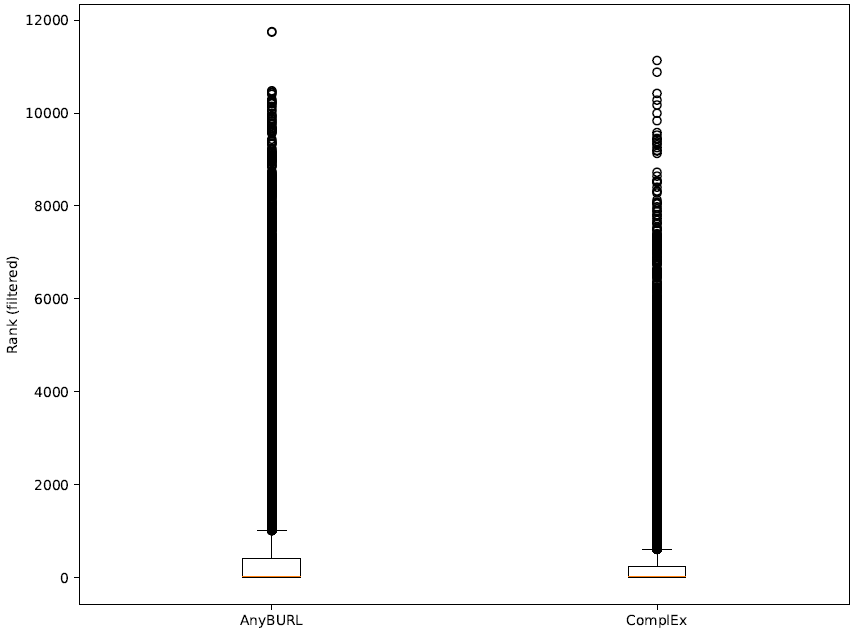
\includegraphics[width=0.9\textwidth]{images/ranks_anyburl_complex_codex.png}
\caption{Comparison of Ranks predicted by AnyBURL and ComplEx for CoDEx-M}
\label{fig:ranks_anyburl_complex_codex}
\end{figure}

If we split up the above boxplot via the prediction direction i.e. whether the head was predicted $(?,r,t)$ or the tail was predicted $(h,r,?)$, as can be seen in figure \ref{fig:ranks_head_tail_anyburl_complex_codex} we can make the same observations as for the figure above: in both prediction directions ComplEx slightly outperforms AnyBURL. Furthermore, we can see that both models are better at predicting the tails while struggling more with the prediction of the heads. 

\begin{figure}[H]
\centering
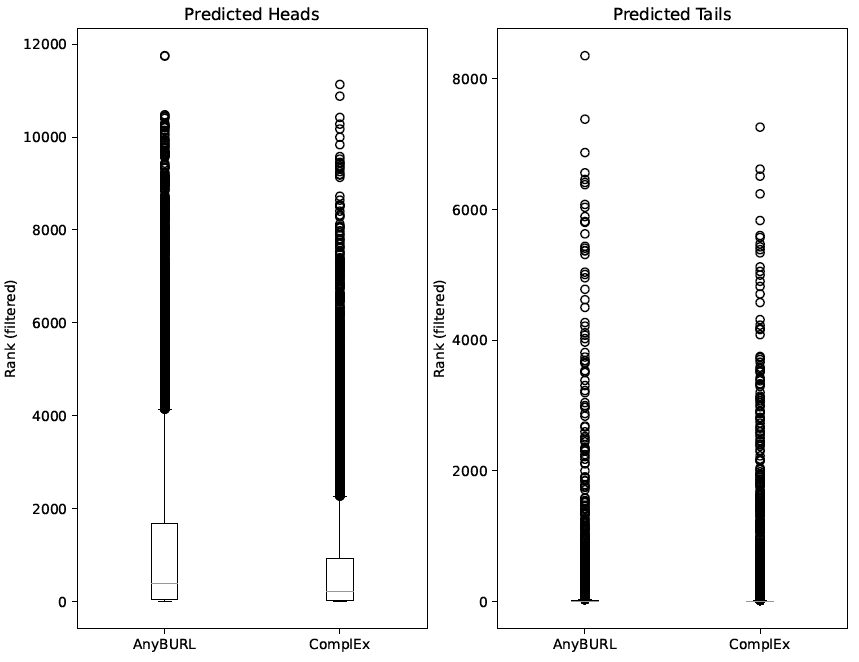
\includegraphics[width=0.9\textwidth]{images/ranks_head_tail_anyburl_complex_codex.png}
\caption{Comparison of Ranks predicted by AnyBURL and ComplEx by prediction direction on CoDEx-M}
\label{fig:ranks_head_tail_anyburl_complex_codex}
\end{figure}

As was to expect the distribution of difference-$\psi$ follows the same pattern as can bee seen in figure \ref{fig:difference_psi_anyburl_complex_codex}. 

\begin{figure}[H]
\centering
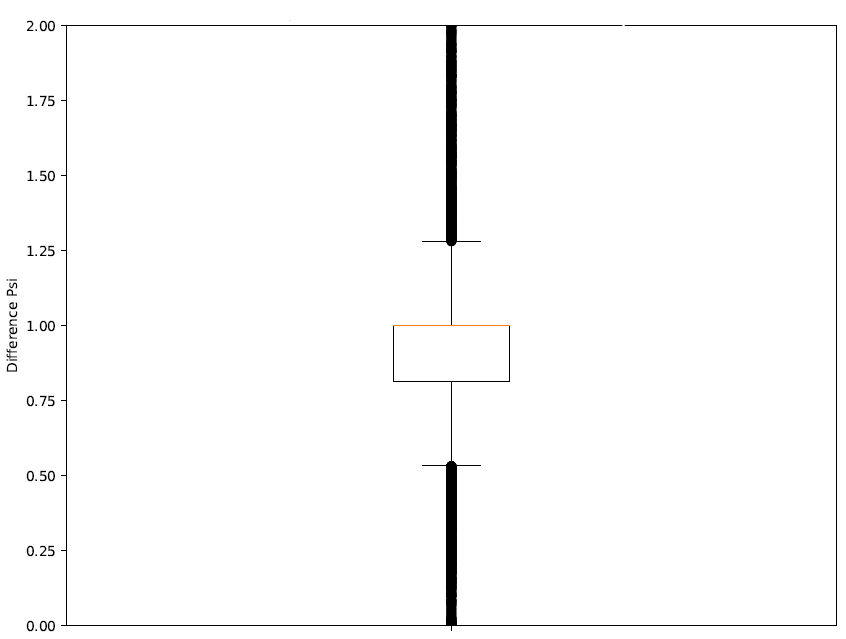
\includegraphics[width=0.9\textwidth]{images/difference_psi_anyburl_complex_codex.png}
\caption{Comparison of difference-$\psi$ between AnyBURL and ComplEx on CoDEx-M}
\label{fig:difference_psi_anyburl_complex_codex}
\end{figure}

If we plot the same graphs for the other model-dataset combinations, we end up with similar results. The corresponding figures can be found in appendix \ref{appendix:rankings}.

The only outlier here are the results for WN18RR. A triple only counts as better predicted by one of the models if difference-$\psi$ is above or below one. The more it deviates from one the stronger the rank difference between the compared models. If we take a look at figure \ref{fig:difference_psi_anyburl_complex_wnrr} we can see that for this model-dataset combination only outliers deviate significantly from one. For my comparison I am mostly interested in the cases where one model predicts a triple better than the other. Given that there are only a few cases for WN18RR, this is one of the main reasons why this dataset proved not very useful for my comparison. To elaborate on this point a bit more the figure does not show that both models predict WN18RR always perfect but the figure shows that both models predict the true answer always on a similar rank and therefore shows us that there are triples in the test dataset which seem to be easier to predict than others for all models. 

\begin{figure}[H]
\centering
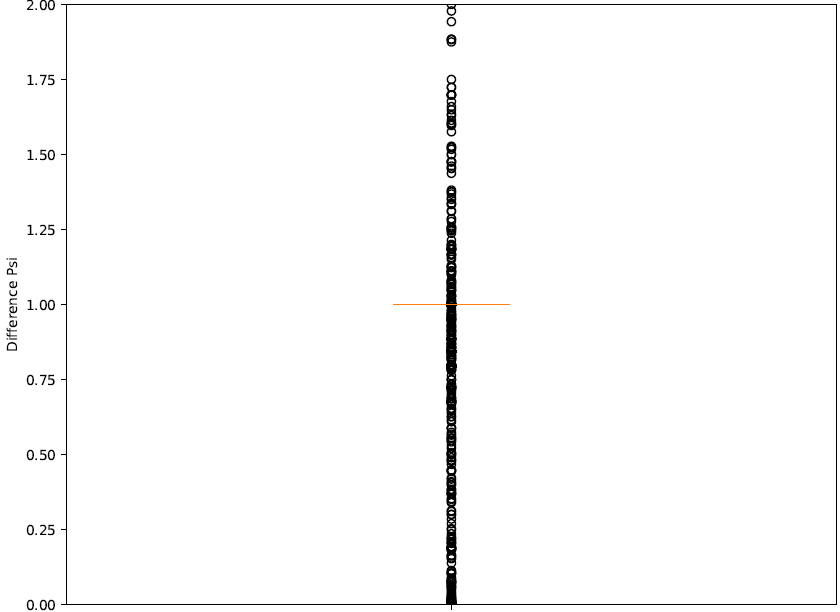
\includegraphics[width=0.9\textwidth]{images/difference_psi_anyburl_complex_wnrr.PNG}
\caption{Comparison of difference-$\psi$ between AnyBURL and ComplEx on WN18RR}
\label{fig:difference_psi_anyburl_complex_wnrr}
\end{figure}

To sum up the results of the comparison of the overall performance comparison, we saw that for all datasets except for WN18RR the sub-symbolic approach performed slightly better than the symbolic approach. The consequence of this is that our data is also slightly skewed in favour of the sub-symbolic models. For that reason when we compare the models based on the difference-$\psi$ value we need to take that into consideration.

\section{Better Predicted by \& Thresholds}
I decided to expand my dataset by a further variable called better $\_predicted\_by\_anyburl$ which transforms the difference-$\psi$ values into a ternary variable. While the size of the deviation from one of difference-$\psi$ encodes some information, this variable discards this part of the information in favour of creating a simpler variable which is easier to understand, interpret and work with. $better\_predicted\_by\_anyburl$ can obtain three values:

\begin{itemize}
\item $-1$ if ranking produced by the embedding-based model is significantly better,
\item $0$ if both models performed equally or 
\item $1$ if AnyBURLs ranking is significantly better.
\end{itemize}

An open question here is how to define significantly better. To find an answer I created the variable based on different thresholds and compared the results. The threshold here is the amount which difference-$\psi$ has to deviate at least from one to not count as an equally good performance any more. The distribution of $better\_predicted\_by\_anyburl$ for different thresholds can be seen in figure \ref{fig:difference_psi_threshold_anyburl_complex_codex}. Here we can notice that if the threshold goes slightly above $0$ the amount of triples equally good predicted by both models increases a lot. If we increase the threshold further from $5$ to $10$ or $25$ the amount of equally good predicted triples increases while the amount of better predicted triples decreases by a similar amount for both models. Above $50$ almost all triples are labelled as equally good predicted while the amount of better predicted triples per model seem to equalize. Furthermore if the threshold is set to $100$ there are no triples better predicted by ComplEx. Here we see a small short coming of the difference-$\psi$ formula. Since two confidence values get divided the result can be at a minimum $0$ while the maximum value of difference-$\psi$ goes against $\infty$. 

\begin{figure}[H]
\centering
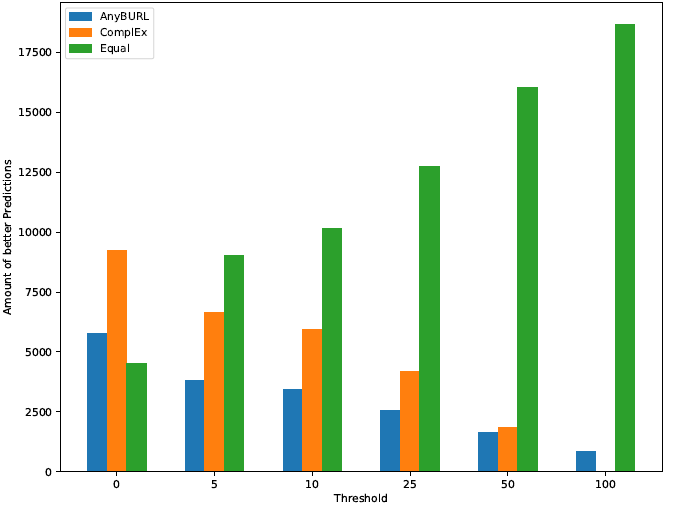
\includegraphics[width=0.9\textwidth]{images/difference_psi_threshold_anyburl_complex_codex.PNG}
\caption{Comparison of different thresholds for the $better\_predicted\_by$ variable}
\label{fig:difference_psi_threshold_anyburl_complex_codex}
\end{figure}

In the end I decided to use $20$ as the final threshold because a value lower than that leaves in my opinion to many cases where the ranks produced by both models were quiet close as better predicted by one of the models. A value above $20$ on the other hand puts to many cases into to the equal bin and since for my comparison the cases where a triple is better predicted by one model are more interesting, keeping as many cases out of the equal bin seemed rational. 

Nevertheless I also generated the comparisons with higher and lower thresholds and noticed that as long as the threshold does not get set to an extreme value (close to $0$ or above $50$) the results do not change significantly.

\section{Comparison based on Characteristics}
In the following the models will be compared in regard to the characteristics defined in the section \ref{sec:research_questions}.

\subsection{Relation Class}
The first characteristic I want to investigate is the relation class of a triple. Bordes \cite{bordes_translating_2013} defines four relation classes "1-To-1", "1-To-Many", "Many-To-1" and "Many-To-Many" or as I will refer them to \textit{1-1}, \textit{1-N}, \textit{M-1} and \textit{M-N}. These relation classes categorize the relations according to the cardinalities of their head and tail entities. For example a relation gets put in to the \textit{1-1} category if a head can appear with at most one tail and the head does also not appear with any other tail. 

Before we can determine whether a certain approach performs better than the other in regard to a specific relation class it first needs to be determined if certain relations get better predicted by one of the approaches. For that I averaged the "$better\_predicted\_by$" variable per relation. The closer the average is to $1$ the more likely it is that AnyBURL is better in predicting this relation and the closer the value is to $-1$ the more likely it is that the sub-symbolic approach is better in predicting this relation. A value of $0$ or close to $0$ would indicate that both models perform equally good in regard to this relation.

If we now plot the averaged $better\_predicted\_by$ values per relation for AnyBURL and ComplEx on CoDEx-M and overlay the relation class category we get figure \ref{fig:relation_class_anyburl_complex_codex}. One the first things one notices when looking at the figure is that all \textit{1-1} relations have a value above $0$, meaning that (almost) all triples containing a relation of that category get better predicted by AnyBURL in comparison to ComplEx. Furthermore, we can see that the \textit{M-1} relations seem evenly distributed and that most relations belonging to the \textit{M-N} category get better predicted by ComplEx. Another interesting takeaway from this figure is that for some reason CoDEx-M does not contain any relations belonging to the \textit{1-N} relation class. 

\begin{figure}[H]
\centering
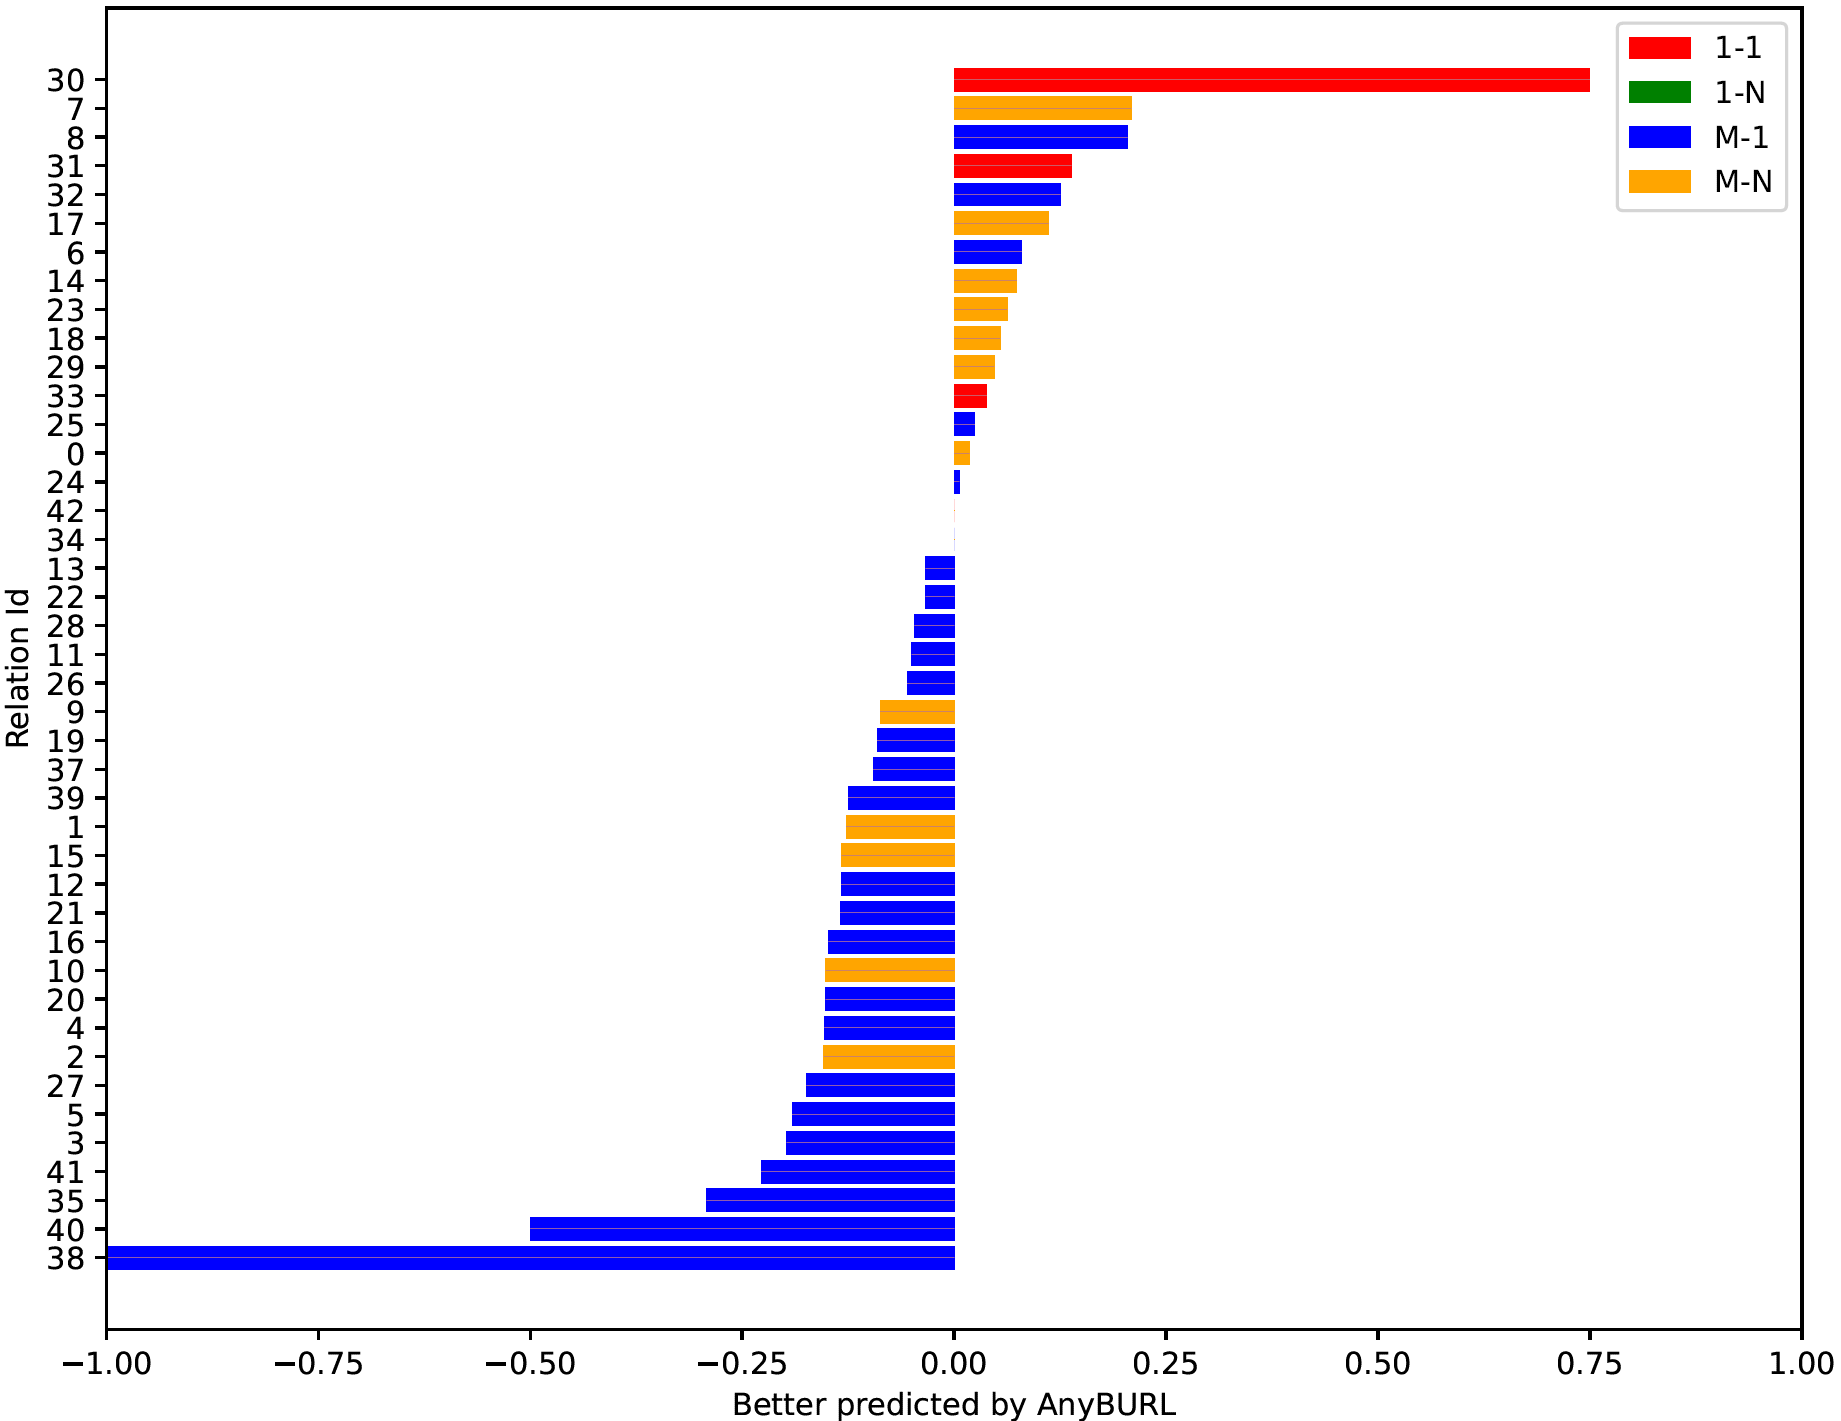
\includegraphics[width=0.9\textwidth]{images/relation_class_anyburl_complex_codex.PNG}
\caption{Comparison of AnyBURL and ComplEx on CoDEx-M in regard to the relation classes}
\label{fig:relation_class_anyburl_complex_codex}
\end{figure}

Since not all relations are equally often represented in the dataset, averaging the $better\_predicted\_by$ value of each triple by their relation distorts the data. To give a better perception of the real data table \ref{tab:relation_class_anyburl_complex_codex} shows the percentage of better predicted triples for each model per relation class. What the previous graph missed to show is that $88.81\%$ of all triples containing a \textit{1-1} relation are equally good predicted by both models while only $10.49\%$ are better predicted by AnyBURL. 

Nevertheless that still indicates that AnyBURL performs better on \textit{1-1} relations but in a less significant manner. 

Moreover, the table shows us that ComplEx predicts roughly $10\%$ more triples of the \textit{M-1} and \textit{M-N} category better than AnyBURL. Here we have to take into account that AnyBURL performed overall slightly worse than ComplEx. Therefore, in my opinion the data indicates that AnyBURL is better in predicting triples with \textit{1-1} relations while only hinting that the same goes for ComplEx and \textit{M-1} and \textit{M-N} relations.

\begin{table}[H]
\centering
\begin{tabular}{c|rrr}
\multicolumn{1}{l|}{} & \multicolumn{1}{c}{\textbf{AnyBURL}} & \multicolumn{1}{c}{\textbf{ComplEx}} & \multicolumn{1}{l}{\textbf{Equal}} \\ \hline
\textbf{1-1} & 10.49\% & 0.7\% & 88.81\% \\
\textbf{1-N} & 0\% & 0\% & 0\% \\
\textbf{M-1} & 11.44\% & 21.66\% & 66.9\% \\
\textbf{M-N} & 16.01\% & 25.82\% & 58.18\%
\end{tabular}
\caption{Percentage of better predicted triples per category by AnyBURL and ComplEX on CoDEx-M}
\label{tab:relation_class_anyburl_complex_codex}
\end{table}

In table \ref{tab:relation_class_anyburl_complex_codex} all data points containing a relation of the \textit{1-N} class are in that category. During the evaluation on the test dataset every triple gets used twice. Once of predicting the head and once for predicting the tail. When predicting the head of an \textit{1-N} relation its essentially like predicting the tail of an \textit{M-1} relation. Therefore I assigned all cases of the \textit{1-N} category where the head was predicted to the \textit{M-1} category. In case CoDEx-M had contained any \textit{M-1} relations I would have done the same swap there as well. The result of this can be found in table \ref{tab:relation_class_cleaned_anyburl_complex_codex}. This corrections does not lead to any new findings the same interpretation of the numbers for the \textit{1-N} and \textit{M-N} relation classes now goes for the \textit{M-1} class as well.

\begin{table}[H]
\centering
\begin{tabular}{c|rrr}
\multicolumn{1}{l|}{} & \multicolumn{1}{c}{\textbf{AnyBURL}} & \multicolumn{1}{c}{\textbf{ComplEx}} & \multicolumn{1}{l}{\textbf{Equal}} \\ \hline
\textbf{1-1} & 10.49\% & 0.7\% & 88.81\% \\
\textbf{1-N} & 16.01\% & 31.14\% & 52.85\% \\
\textbf{M-1} & 7.24\% & 12.91\% & 79.85\% \\
\textbf{M-N} & 16.01\% & 25.82\% & 58.18\%
\end{tabular}
\caption{Percentage of better predicted triples per category by AnyBURL and ComplEX on CoDEx-M with fixed relation class assignments}
\label{tab:relation_class_cleaned_anyburl_complex_codex}
\end{table}

Comparing ConvE and RESCAL to AnyBURL in regard to the relation classes results in a similar outcome. This can be seen in figure \ref{fig:relation_class_anyburl_conve_rescal_codex} and tables \ref{tab:relation_class_cleaned_anyburl_conve_codex} and \ref{tab:relation_class_cleaned_anyburl_rescal_codex}. This shows us that my previous observations are not only valid for one model sub-symbolic model but for multiple and therefore maybe for the whole approach.

A slight take back here is the strong variations in the tables. While all tables display comparable results they do so in varying magnitudes. While AnyBURL only predicts $10\%$ of the \textit{1-1} relations better than ComplEx (table \ref{tab:relation_class_cleaned_anyburl_complex_codex}), it predicts $29\%$ better than ConvE (table \ref{tab:relation_class_cleaned_anyburl_conve_codex}) and $81\%$ better than RESCAL (table \ref{tab:relation_class_cleaned_anyburl_rescal_codex}). By further analysing the data I could not determine an explanation for this strong variation.

\begin{figure}[H]
\centering
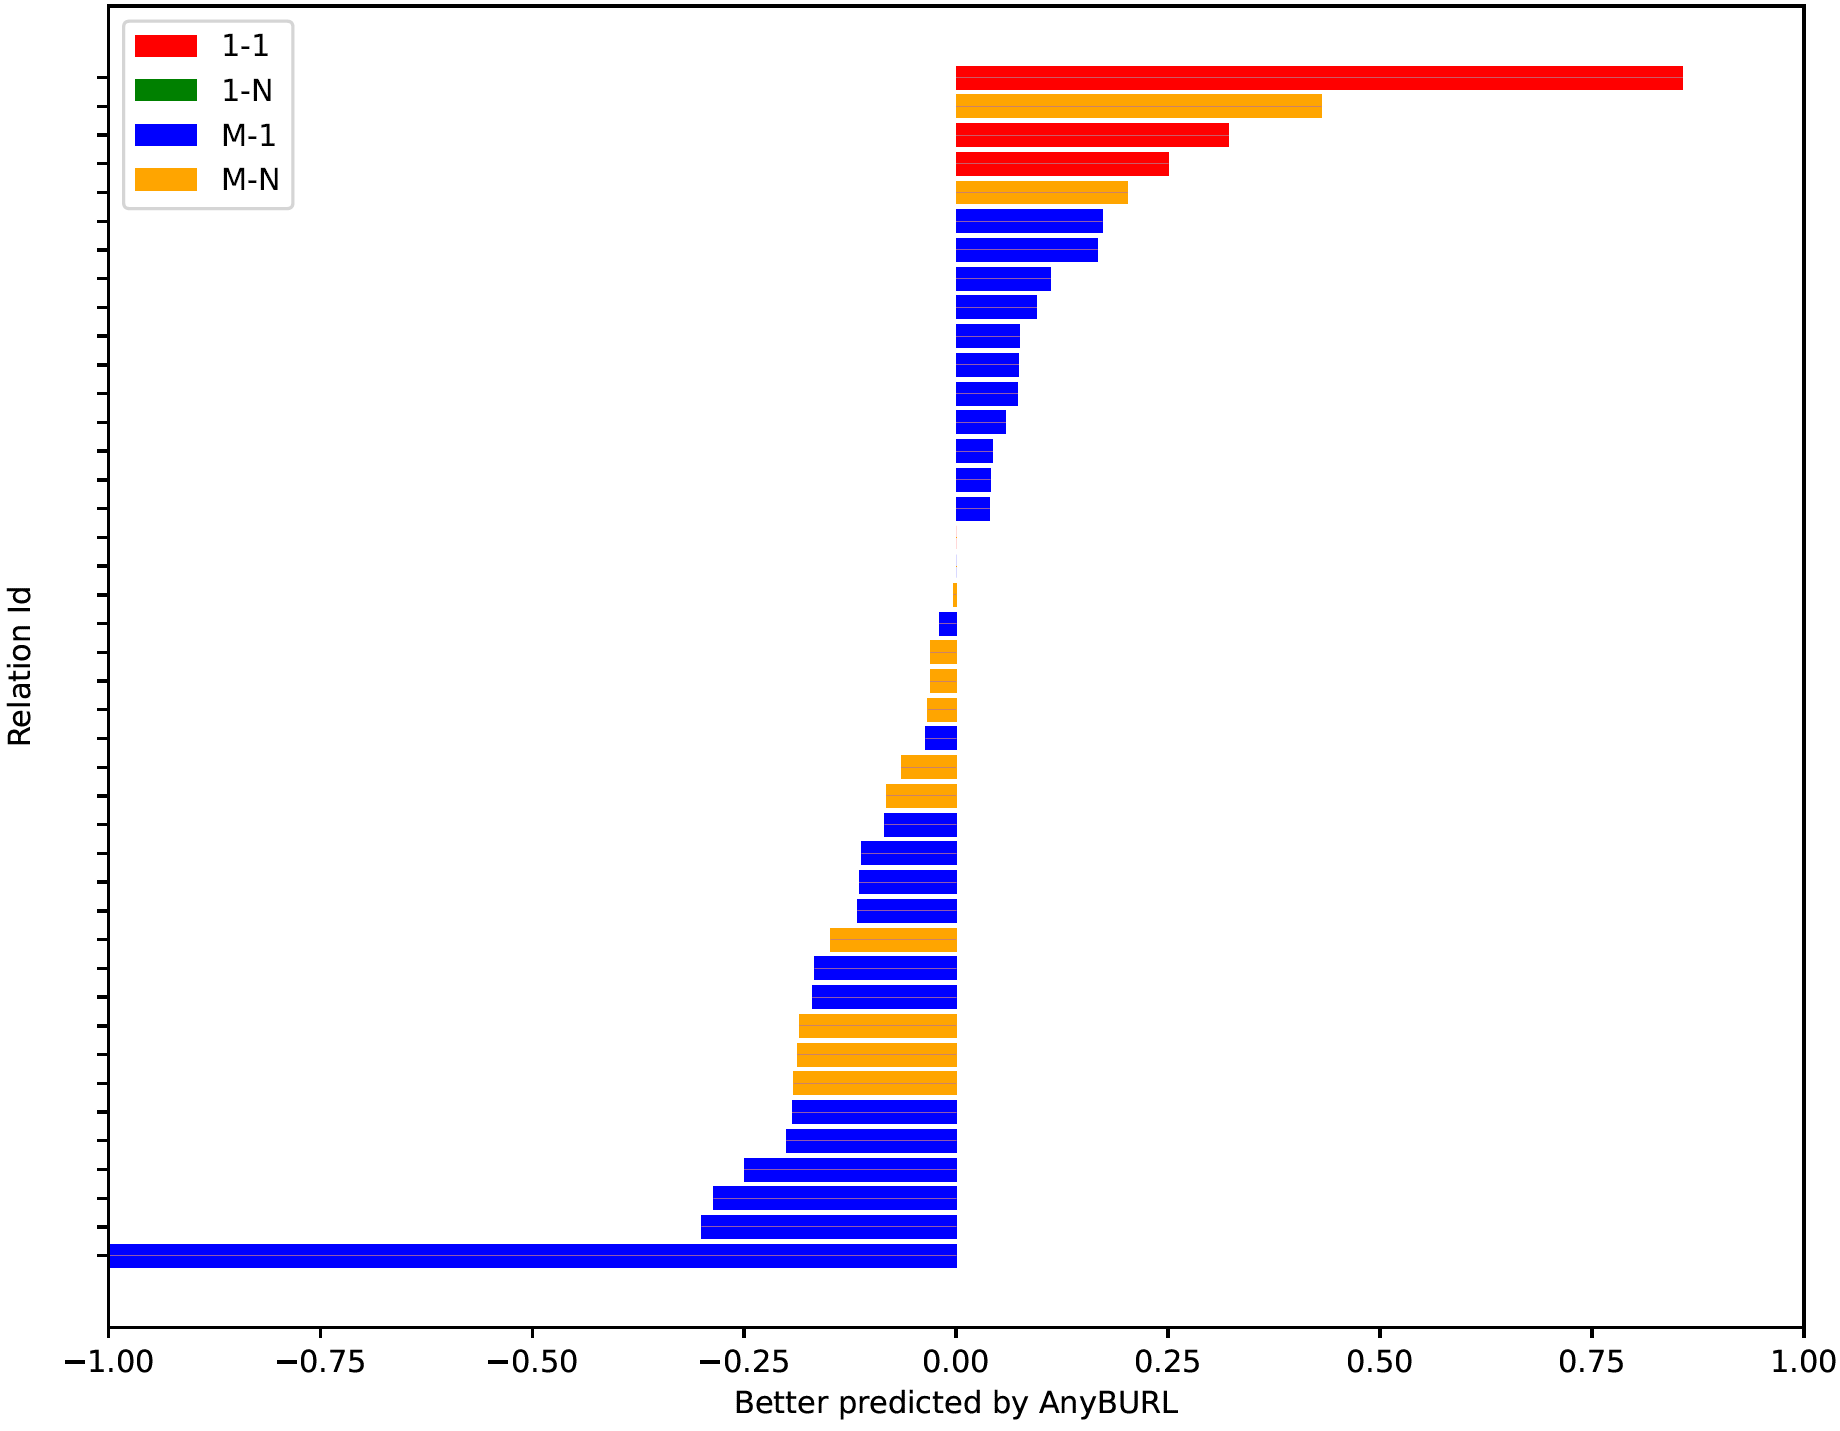
\includegraphics[width=0.45\textwidth]{images/relation_class_anyburl_conve_codex.PNG}
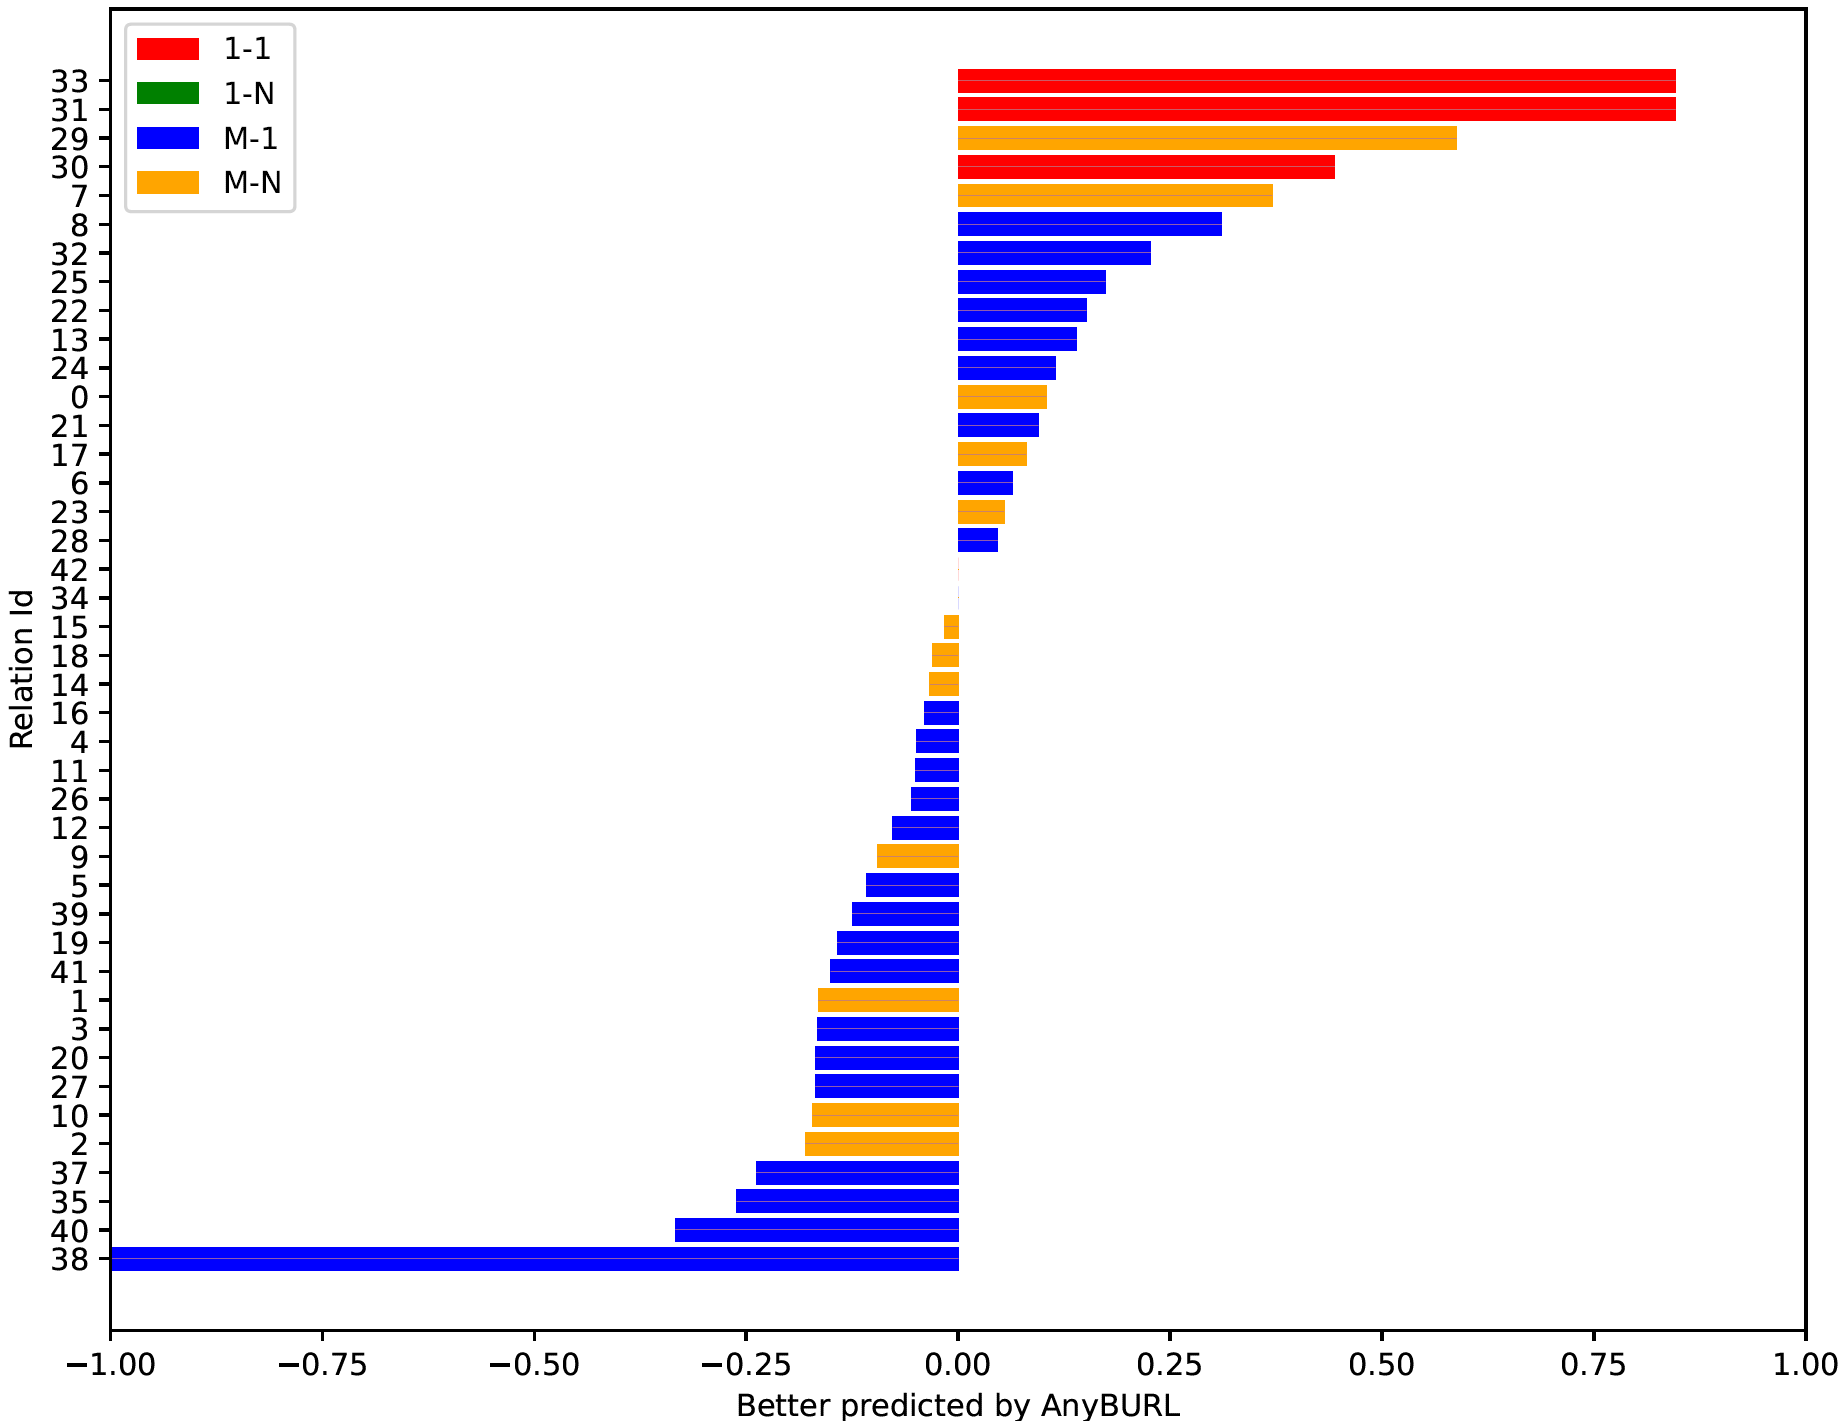
\includegraphics[width=0.45\textwidth]{images/relation_class_anyburl_rescal_codex.PNG}
\caption{Comparison of AnyBURL and ConvE (left) / RESCAL (right) on CoDEx-M in regard to the relation classes}
\label{fig:relation_class_anyburl_conve_rescal_codex}
\end{figure}

\begin{table}[H]
\centering
\begin{tabular}{c|rrr}
\multicolumn{1}{l|}{} & \multicolumn{1}{c}{\textbf{AnyBURL}} & \multicolumn{1}{c}{\textbf{RESCAL}} & \multicolumn{1}{l}{\textbf{Equal}} \\ \hline
\textbf{1-1} & 29.29\% & 0\% & 70.71\% \\
\textbf{1-N} & 22.66\% & 26.19\% & 51.15\% \\
\textbf{M-1} & 9.24\% & 13.21\% & 77.55\% \\
\textbf{M-N} & 15.29\% & 27.94\% & 56.77\%
\end{tabular}
\caption{Percentage of better predicted triples per category by AnyBURL and ConvE on CoDEx-M with fixed relation class assignments}
\label{tab:relation_class_cleaned_anyburl_conve_codex}
\end{table}

\begin{table}[H]
\centering
\begin{tabular}{c|rrr}
\multicolumn{1}{l|}{} & \multicolumn{1}{c}{\textbf{AnyBURL}} & \multicolumn{1}{c}{\textbf{RESCAL}} & \multicolumn{1}{l}{\textbf{Equal}} \\ \hline
\textbf{1-1} & 81.1\% & 0\% & 18.9\% \\
\textbf{1-N} & 18.93\% & 27.65\% & 53.43\% \\
\textbf{M-1} & 13.55\% & 11.42\% & 75.04\% \\
\textbf{M-N} & 15.86\% & 26.24\% & 57.9\%
\end{tabular}
\caption{Percentage of better predicted triples per category by AnyBURL and RESCAL on CoDEx-M with fixed relation class assignments}
\label{tab:relation_class_cleaned_anyburl_rescal_codex}
\end{table}

If creating the same graph (as in figure \ref{fig:relation_class_anyburl_complex_codex} and \ref{fig:relation_class_anyburl_conve_rescal_codex}) for the experiments on FB15k-237, the graph is incomprehensible due to the amount of relations in the dataset. This can be seen in appendix \ref{appendix:relation_class_fb15k}. Therefore in the following I will only refer to the tables for FB15k-237.

First of for ConvE we can make the same observations as before on CodEx-M. As can be seen in table \ref{tab:relation_class_cleaned_anyburl_conve_fb15k}, while ConvE is better than AnyBURL in most relation classes, AnyBURL outperforms ConvE in regard to the \textit{1-1} relation class. 

\begin{table}[H]
\centering
\begin{tabular}{c|rrr}
\multicolumn{1}{l|}{} & \multicolumn{1}{c}{\textbf{AnyBURL}} & \multicolumn{1}{c}{\textbf{ConvE}} & \multicolumn{1}{l}{\textbf{Equal}} \\ \hline
\textbf{1-1} & 21.05\% & 6.58\% & 72.37\% \\
\textbf{1-N} & 16.2\% & 20.68\% & 63.12\% \\
\textbf{M-1} & 7.21\% & 15.89\% & 76.9\% \\
\textbf{M-N} & 11.37\% & 25.29\% & 63.35\%
\end{tabular}
\caption{Percentage of better predicted triples per category by AnyBURL and ConvE on FB15k-237 with fixed relation class assignments}
\label{tab:relation_class_cleaned_anyburl_conve_fb15k}
\end{table}

When looking at the data for ComplEx (table \ref{tab:relation_class_cleaned_anyburl_complex_fb15k}) and RESCAL (table \ref{tab:relation_class_cleaned_anyburl_rescal_fb15k}), we can still see that the embedding-based models outperform AnyBURL in the relation classes \textit{1-N}, \textit{M-1} and \textit{M-N} while they perform similar in the \textit{1-1} category. 
If we take into account here again that the sub-symbolic models generally outperformed AnyBURL, this data still slightly indicates that AnyBURL might be better than the sub-symbolic models in predicting relations of the \textit{1-1} class. 

\begin{table}[H]
\centering
\begin{tabular}{c|rrr}
\multicolumn{1}{l|}{} & \multicolumn{1}{c}{\textbf{AnyBURL}} & \multicolumn{1}{c}{\textbf{ComplEx}} & \multicolumn{1}{l}{\textbf{Equal}} \\ \hline
\textbf{1-1} & 5.66\% & 5.66\% & 88.68\% \\
\textbf{1-N} & 12.45\% & 22.3\% & 65.25\% \\
\textbf{M-1} & 7.04\% & 15.1\% & 77.86\% \\
\textbf{M-N} & 9.57\% & 24.99\% & 65.44\%
\end{tabular}
\caption{Percentage of better predicted triples per category by AnyBURL and ComplEx on FB15k-237 with fixed relation class assignments}
\label{tab:relation_class_cleaned_anyburl_complex_fb15k}
\end{table}

\begin{table}[H]
\centering
\begin{tabular}{c|rrr}
\multicolumn{1}{l|}{} & \multicolumn{1}{c}{\textbf{AnyBURL}} & \multicolumn{1}{c}{\textbf{RESCAL}} & \multicolumn{1}{l}{\textbf{Equal}} \\ \hline
\textbf{1-1} & 8.54\% & 7.54\% & 83.92\% \\
\textbf{1-N} & 14.75\% & 22.57\% & 62.68\% \\
\textbf{M-1} & 7.01\% & 16.03\% & 76.96\% \\
\textbf{M-N} & 10.17\% & 25.71\% & 64.13\%
\end{tabular}
\caption{Percentage of better predicted triples per category by AnyBURL and RESCAL on FB15k-237 with fixed relation class assignments}
\label{tab:relation_class_cleaned_anyburl_rescal_fb15k}
\end{table}

In figure \ref{fig:relation_class_anyburl_complex_yago} we can see that the experiments on YAGO3-10 do not produce the same results as the experiments on CoDEx-M and FB15k-237 did. Here no model seems to be better than the other in regard to any relation class. If we refer to table \ref{tab:relation_class_cleaned_anyburl_complex_yago} we notice that both models seem to perform equal in all relation classes except for the \textit{M-1} class where AnyBURL is better than ComplEx. 

\begin{figure}[H]
\centering
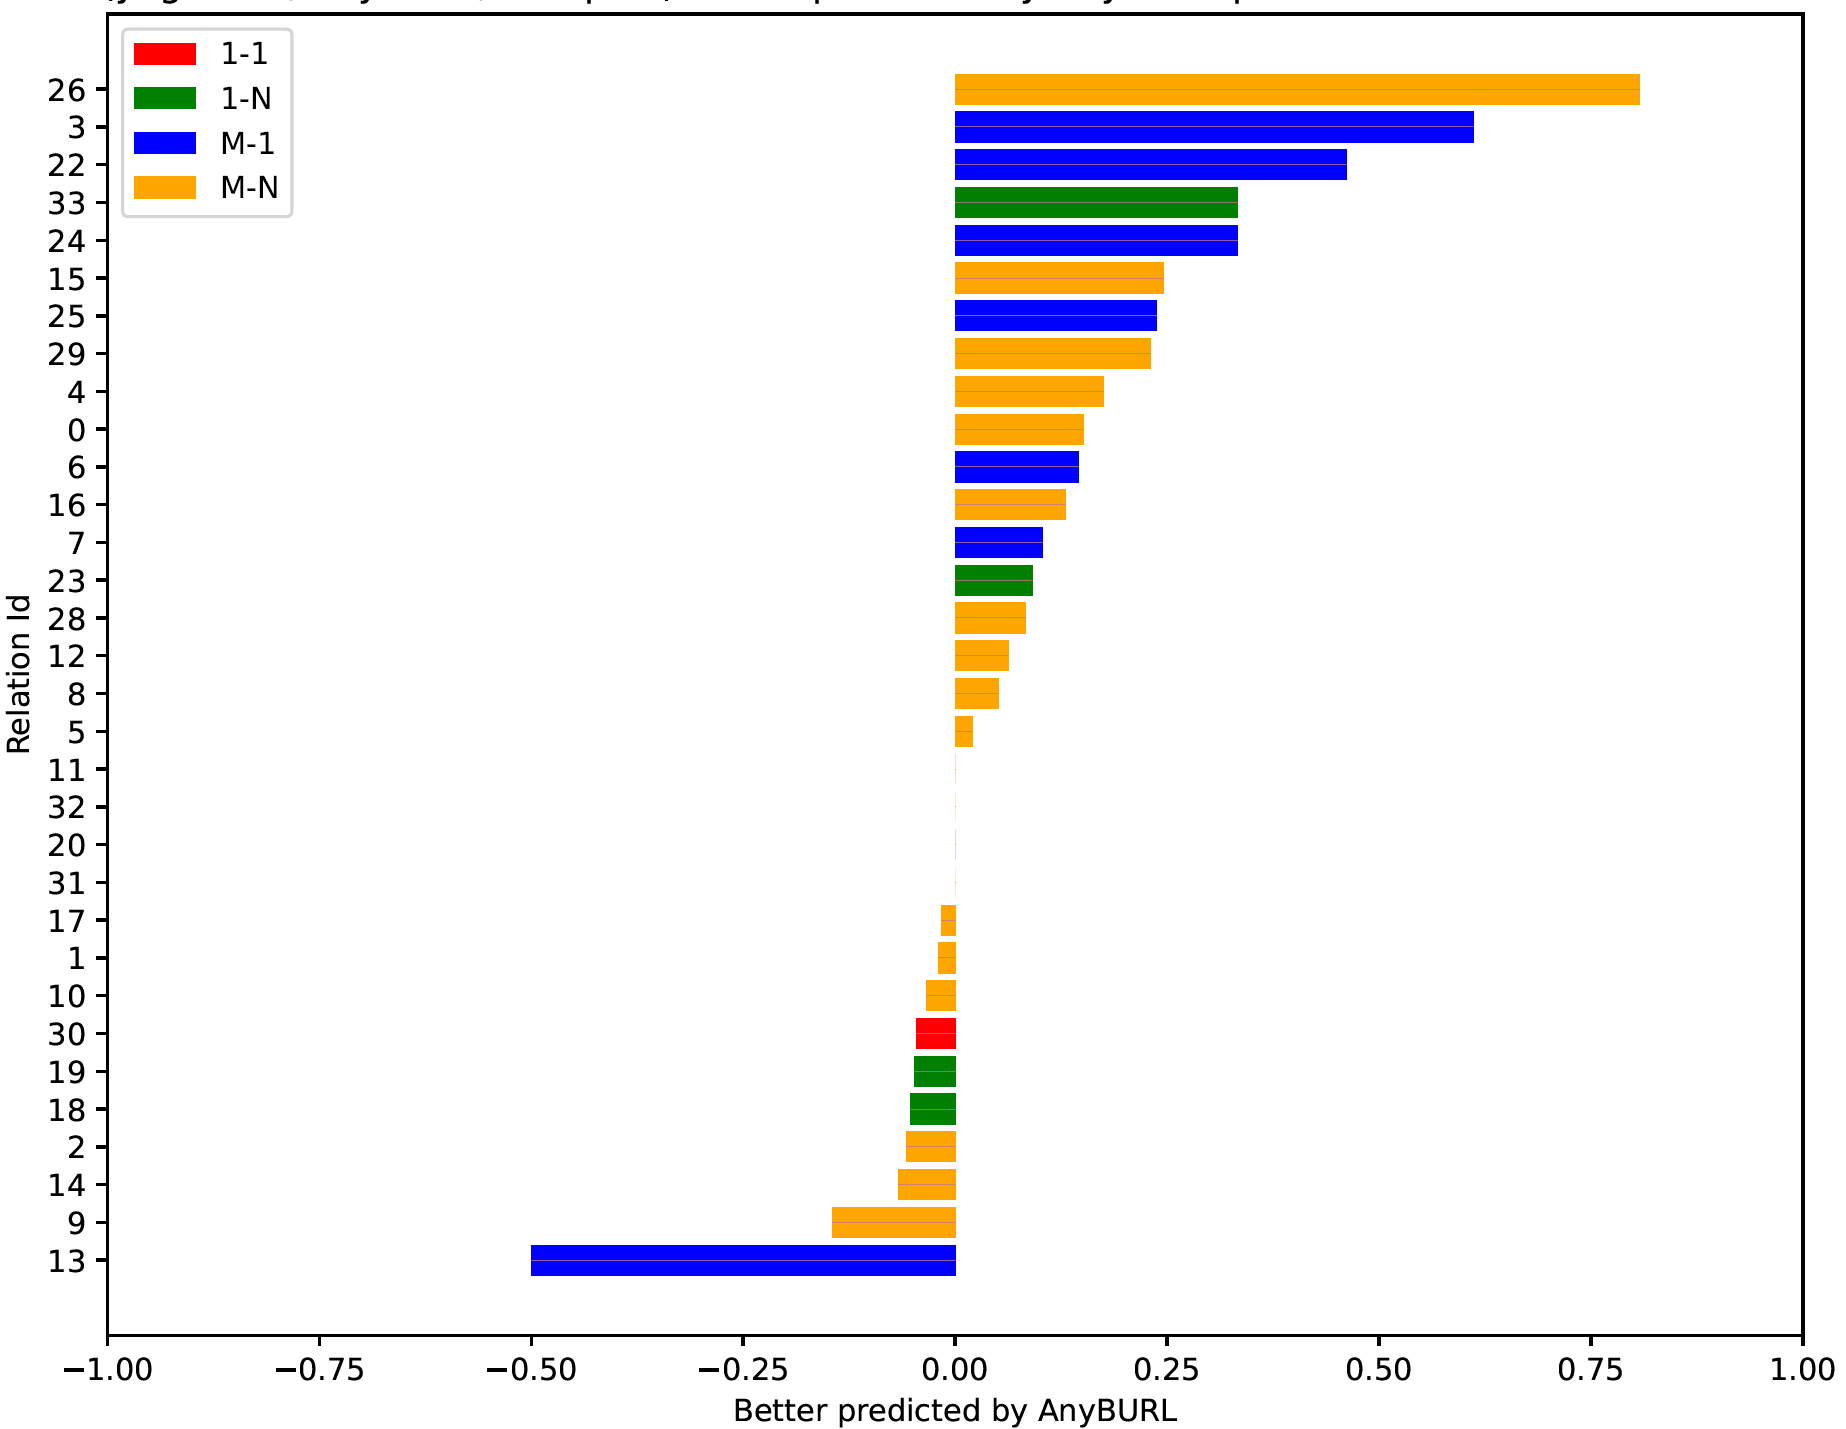
\includegraphics[width=0.9\textwidth]{images/relation_class_anyburl_complex_yago.PNG}
\caption{Comparison of AnyBURL and ComplEx on YAGO3-10 in regard to the relation classes}
\label{fig:relation_class_anyburl_complex_yago}
\end{figure}

\begin{table}[H]
\centering
\begin{tabular}{c|rrr}
\multicolumn{1}{l|}{} & \multicolumn{1}{c}{\textbf{AnyBURL}} & \multicolumn{1}{c}{\textbf{ComplEx}} & \multicolumn{1}{l}{\textbf{Equal}} \\ \hline
\textbf{1-1} & 3.57\% & 5.36\% & 91.07\% \\
\textbf{1-N} & 16.5\% & 15.46\% & 68.04\% \\
\textbf{M-1} & 21.92\% & 6.8\% & 71.28\% \\
\textbf{M-N} & 7.38\% & 8.35\% & 84.28\%
\end{tabular}
\caption{Percentage of better predicted triples per category by AnyBURL and ComplEx on YAGO3-10 with fixed relation class assignments}
\label{tab:relation_class_cleaned_anyburl_complex_yago}
\end{table}

In this section we have now seen that AnyBURL seems to be better in predicting triples with \textit{1-1} relations while the sub-symbolic models favour relations with a multi-cardinality. On the CoDEx-M dataset the data showed this almost unambiguously and on FB15k-237 the data showed the same result but not as clearly as on CoDEx-M. YAGO3-10 is an outlier here, on this dataset both models performed equally good in regard to the relation classes.

\subsection{Relation Frequency in Trainings Data}
The next characteristic I want to investigate is the relation frequency in the trainings data. To be more specific, in figure \ref{fig:relation_freq_codex} we can see that in CoDEx-M some relations occur more often than others in the trainings data, therefore I wanted to see whether one approach might be better than the other in predicting triples containing less often occurring relations or containing often occurring relations. In appendix \ref{appendix:relation_freq} the same graph can be seen for FB15k-237 and YAGO3-10 which also show that some relations are more frequent than others in these datasets. 

\begin{figure}[H]
\centering
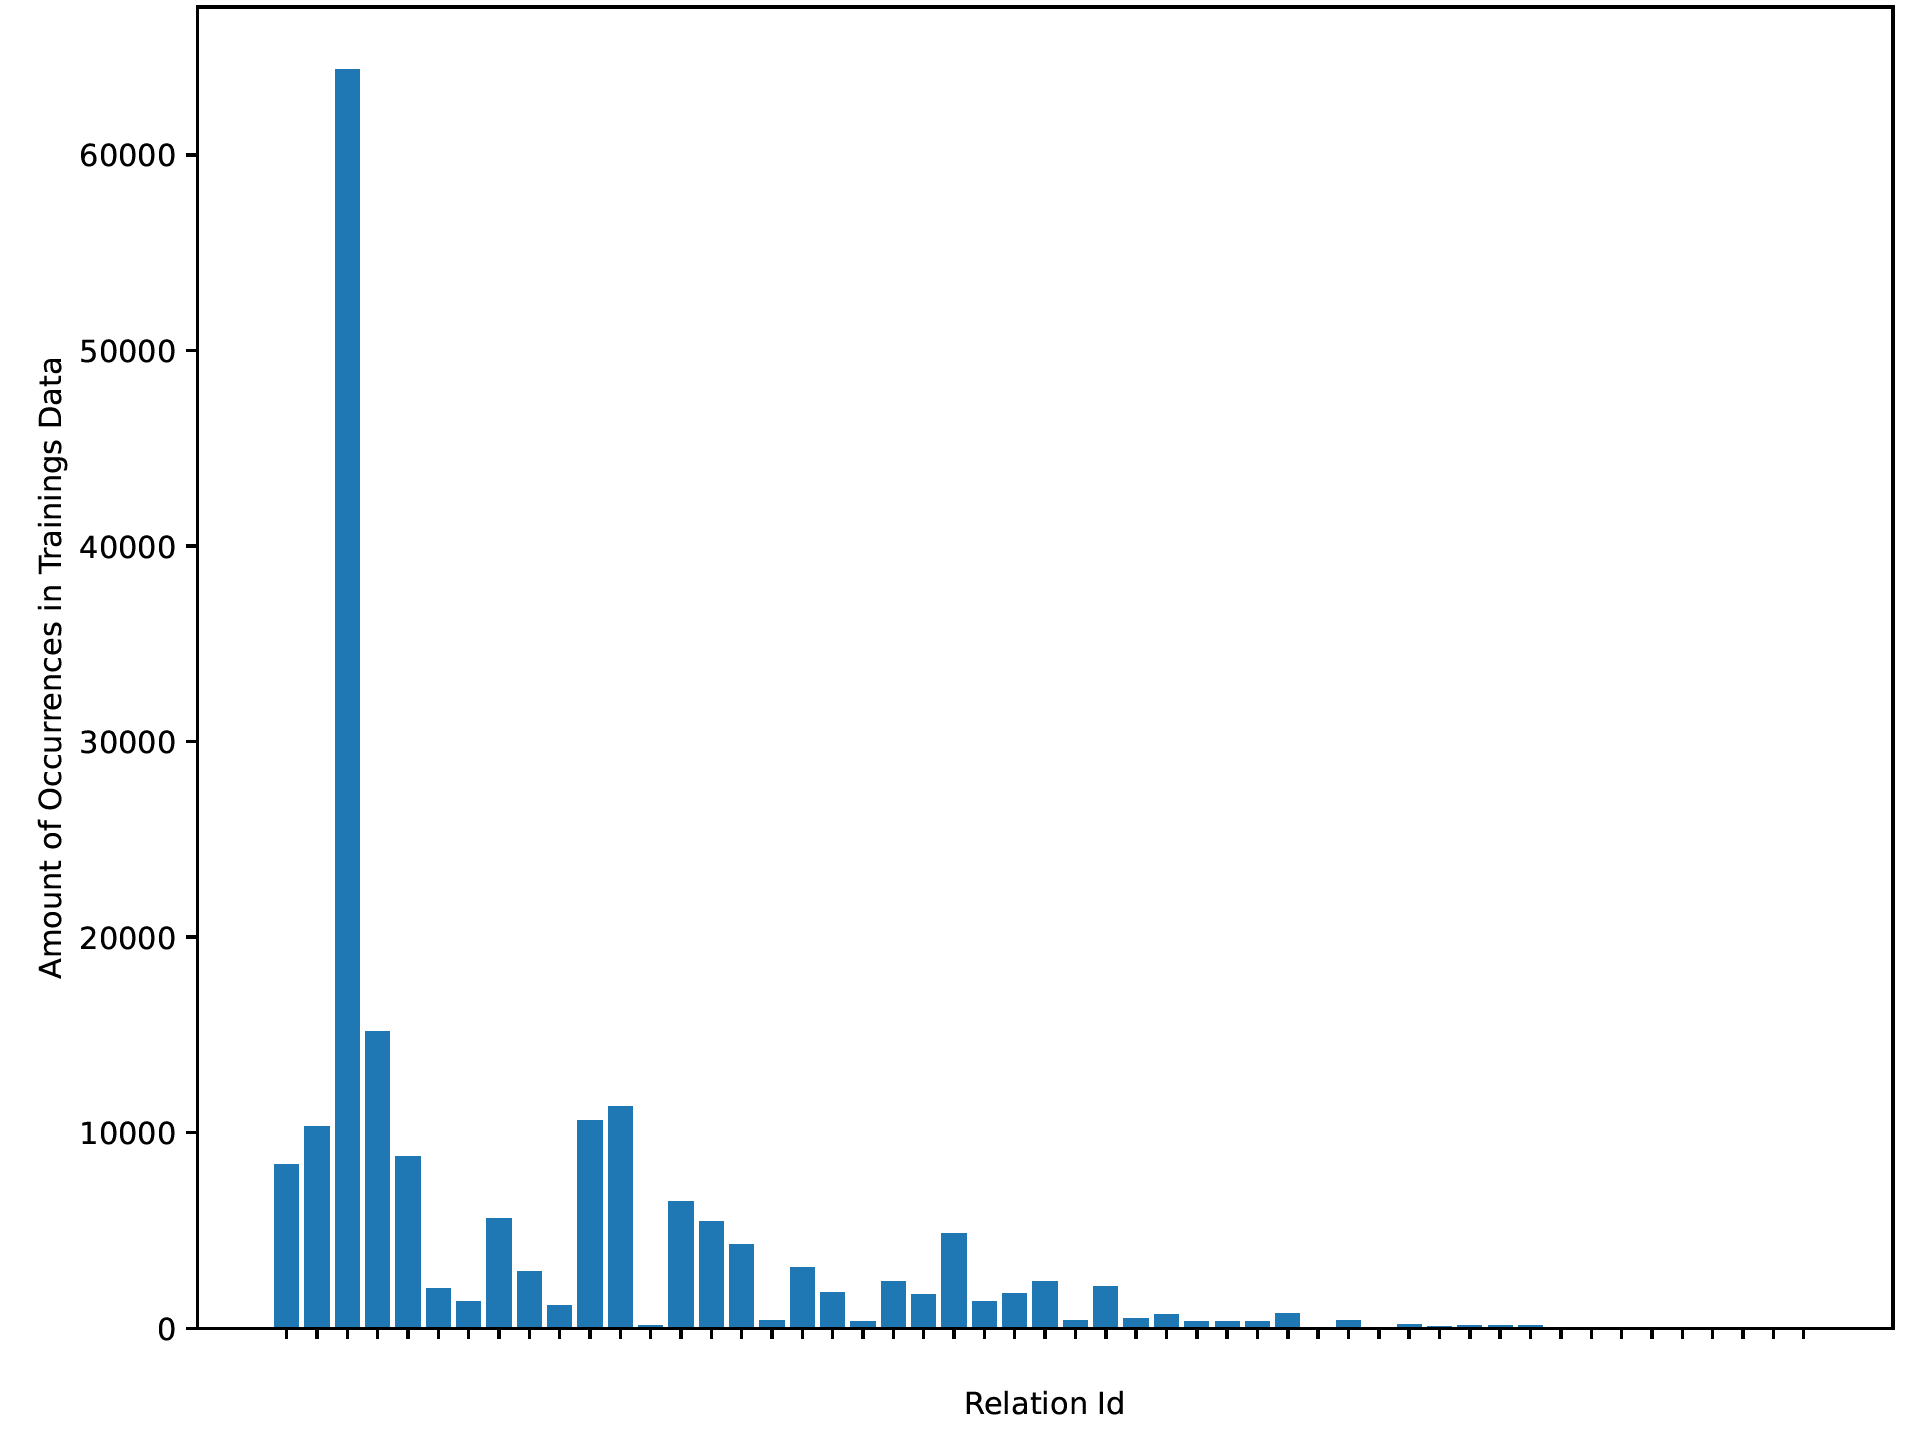
\includegraphics[width=0.9\textwidth]{images/relation_freq_codex.PNG}
\caption{Relation frequency in trainings data for CoDEx-M}
\label{fig:relation_freq_codex}
\end{figure}

In figure \ref{fig:relation_freq_anyburl_complex_codex} the relation frequency data is normalized between $0$ and $1$ overlayed on the per relation aggregated $better\_predicted\_by$ data, the same aggregation as in the previous section. Important to note before viewing this graph is that as we can see on the scale on the right the colouring of the bars is not evenly spread out along the range of the normalized frequency data. Instead I set the maximum of the color scale to the second most frequent relation. Because the most frequent relation is extremely dominant, the colors of the other bars would otherwise be almost indistinguishably. 

In this graph AnyBURL and ComplEx are compared on CoDEx-M. We notice here that the six most frequent relations are all better predicted by ComplEx. While only a few somewhat frequent relations are better predicted by AnyBURL. 

This observation has two limitations. For once there are only a handful of relations which can be counted as frequently occurring and furthermore the frequent relations better predicted by ComplEx all have an average $better\_predicted\_by$ value smaller than $-0.25$. This shows us that there is no strong correlation and we can only assume a slight connection between the relation frequency and the performance of both approaches.

\begin{figure}[H]
\centering
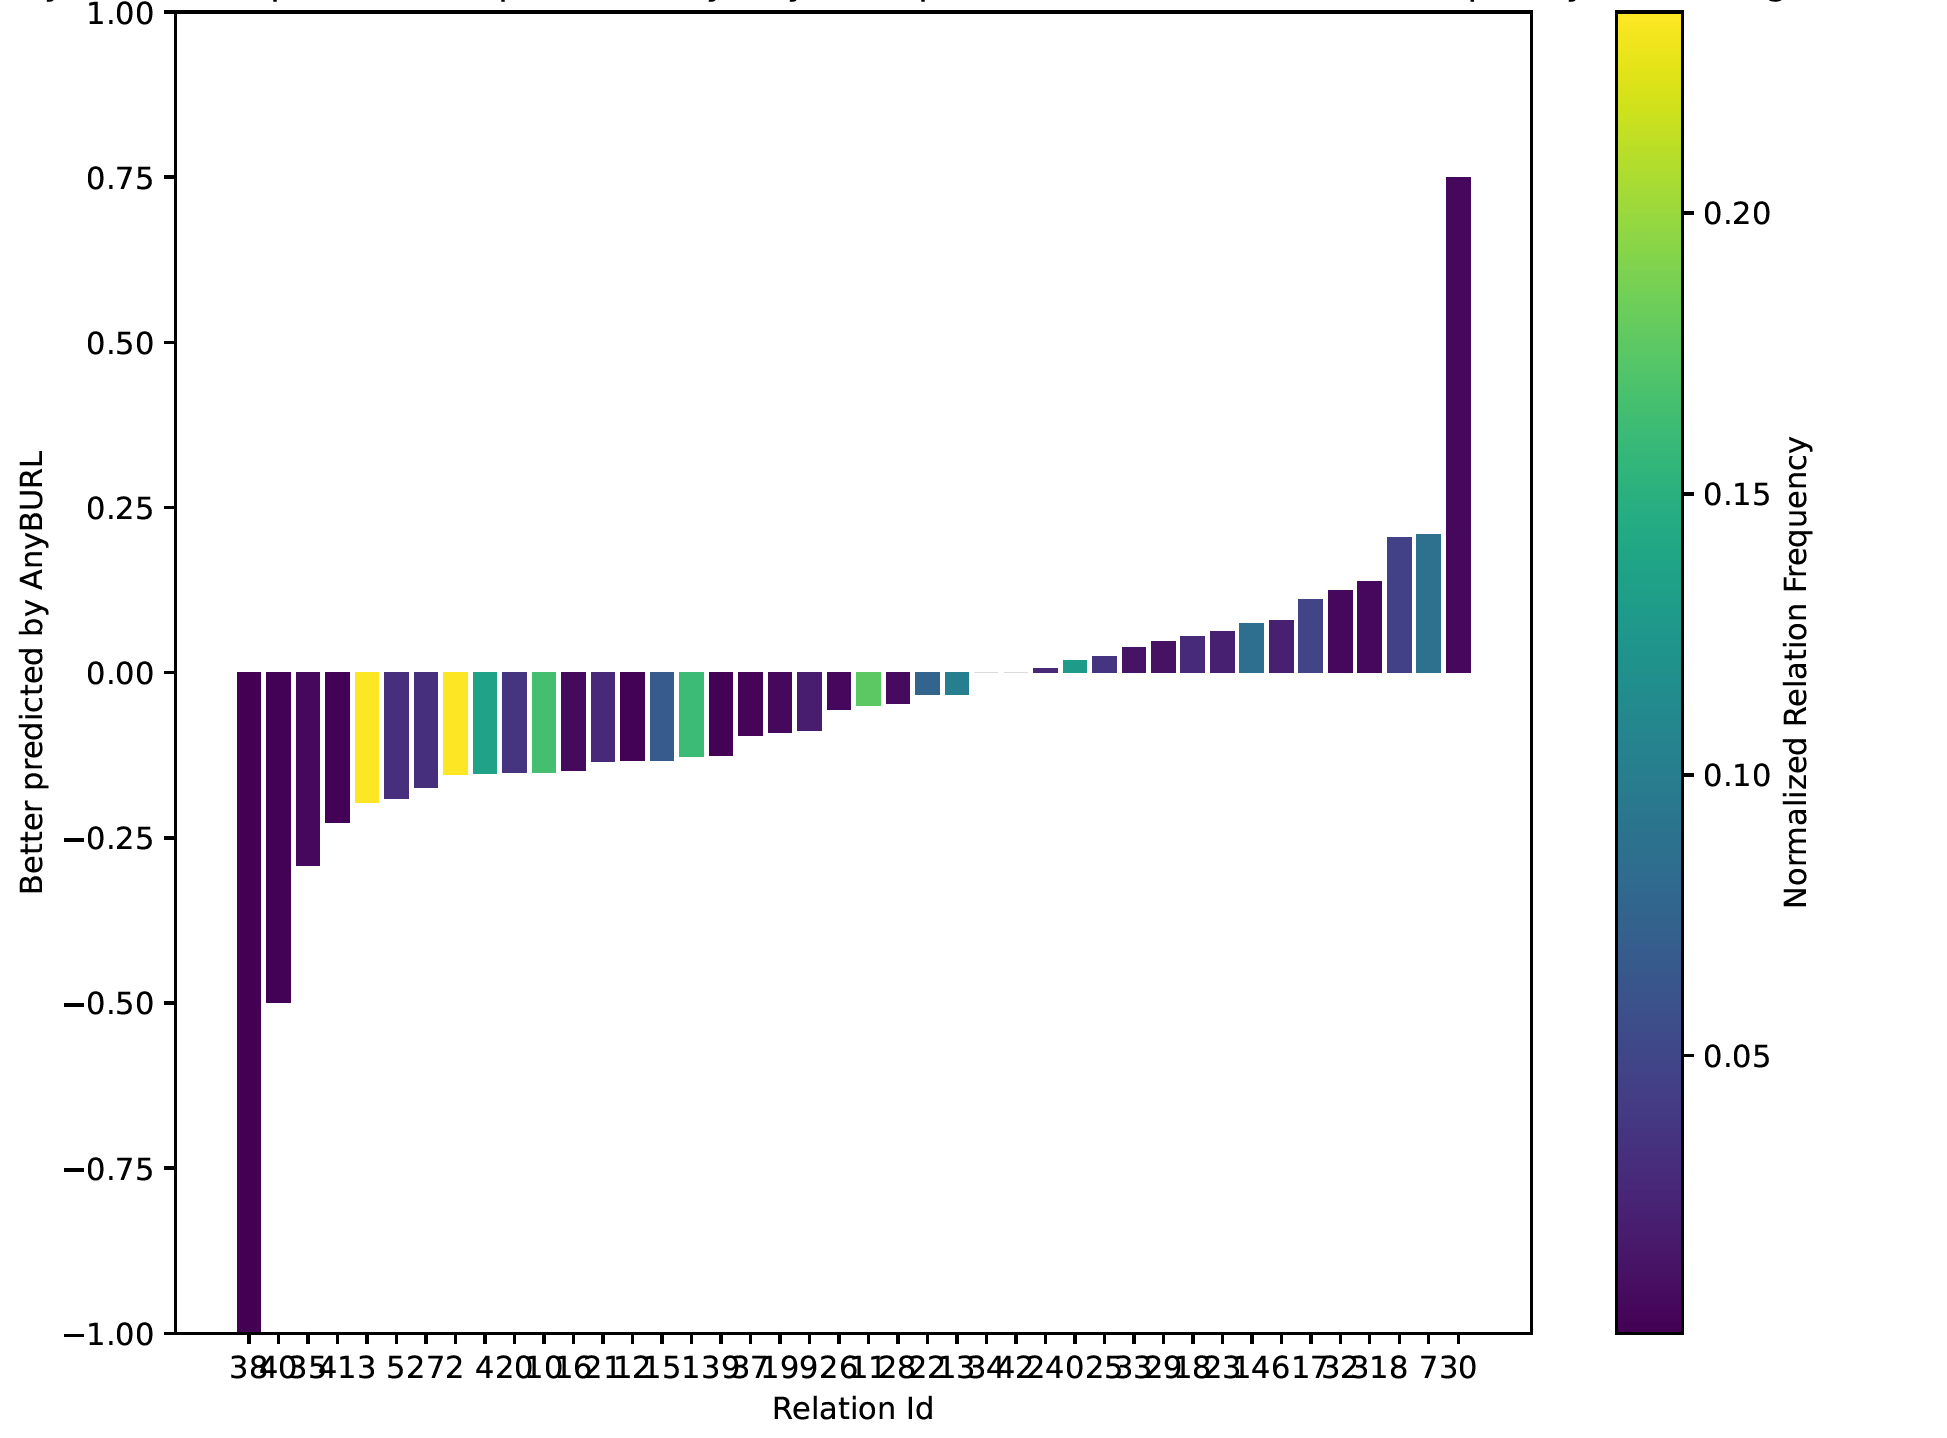
\includegraphics[width=0.9\textwidth]{images/relation_freq_anyburl_complex_codex.PNG}
\caption{Comparison of AnyBURL and ComplEx on CoDEx-M in regard to the relation frequency}
\label{fig:relation_freq_anyburl_complex_codex}
\end{figure}

When plotting the same graph for ConvE and RESCAL, as can be seen in figure \ref{fig:relation_freq_anyburl_conve_rescal_codex}, we notice that here the most frequent relations are all better predicted by the embedding-based models than by AnyBURL. But the same limitations as before also hold.

\begin{figure}[H]
\centering
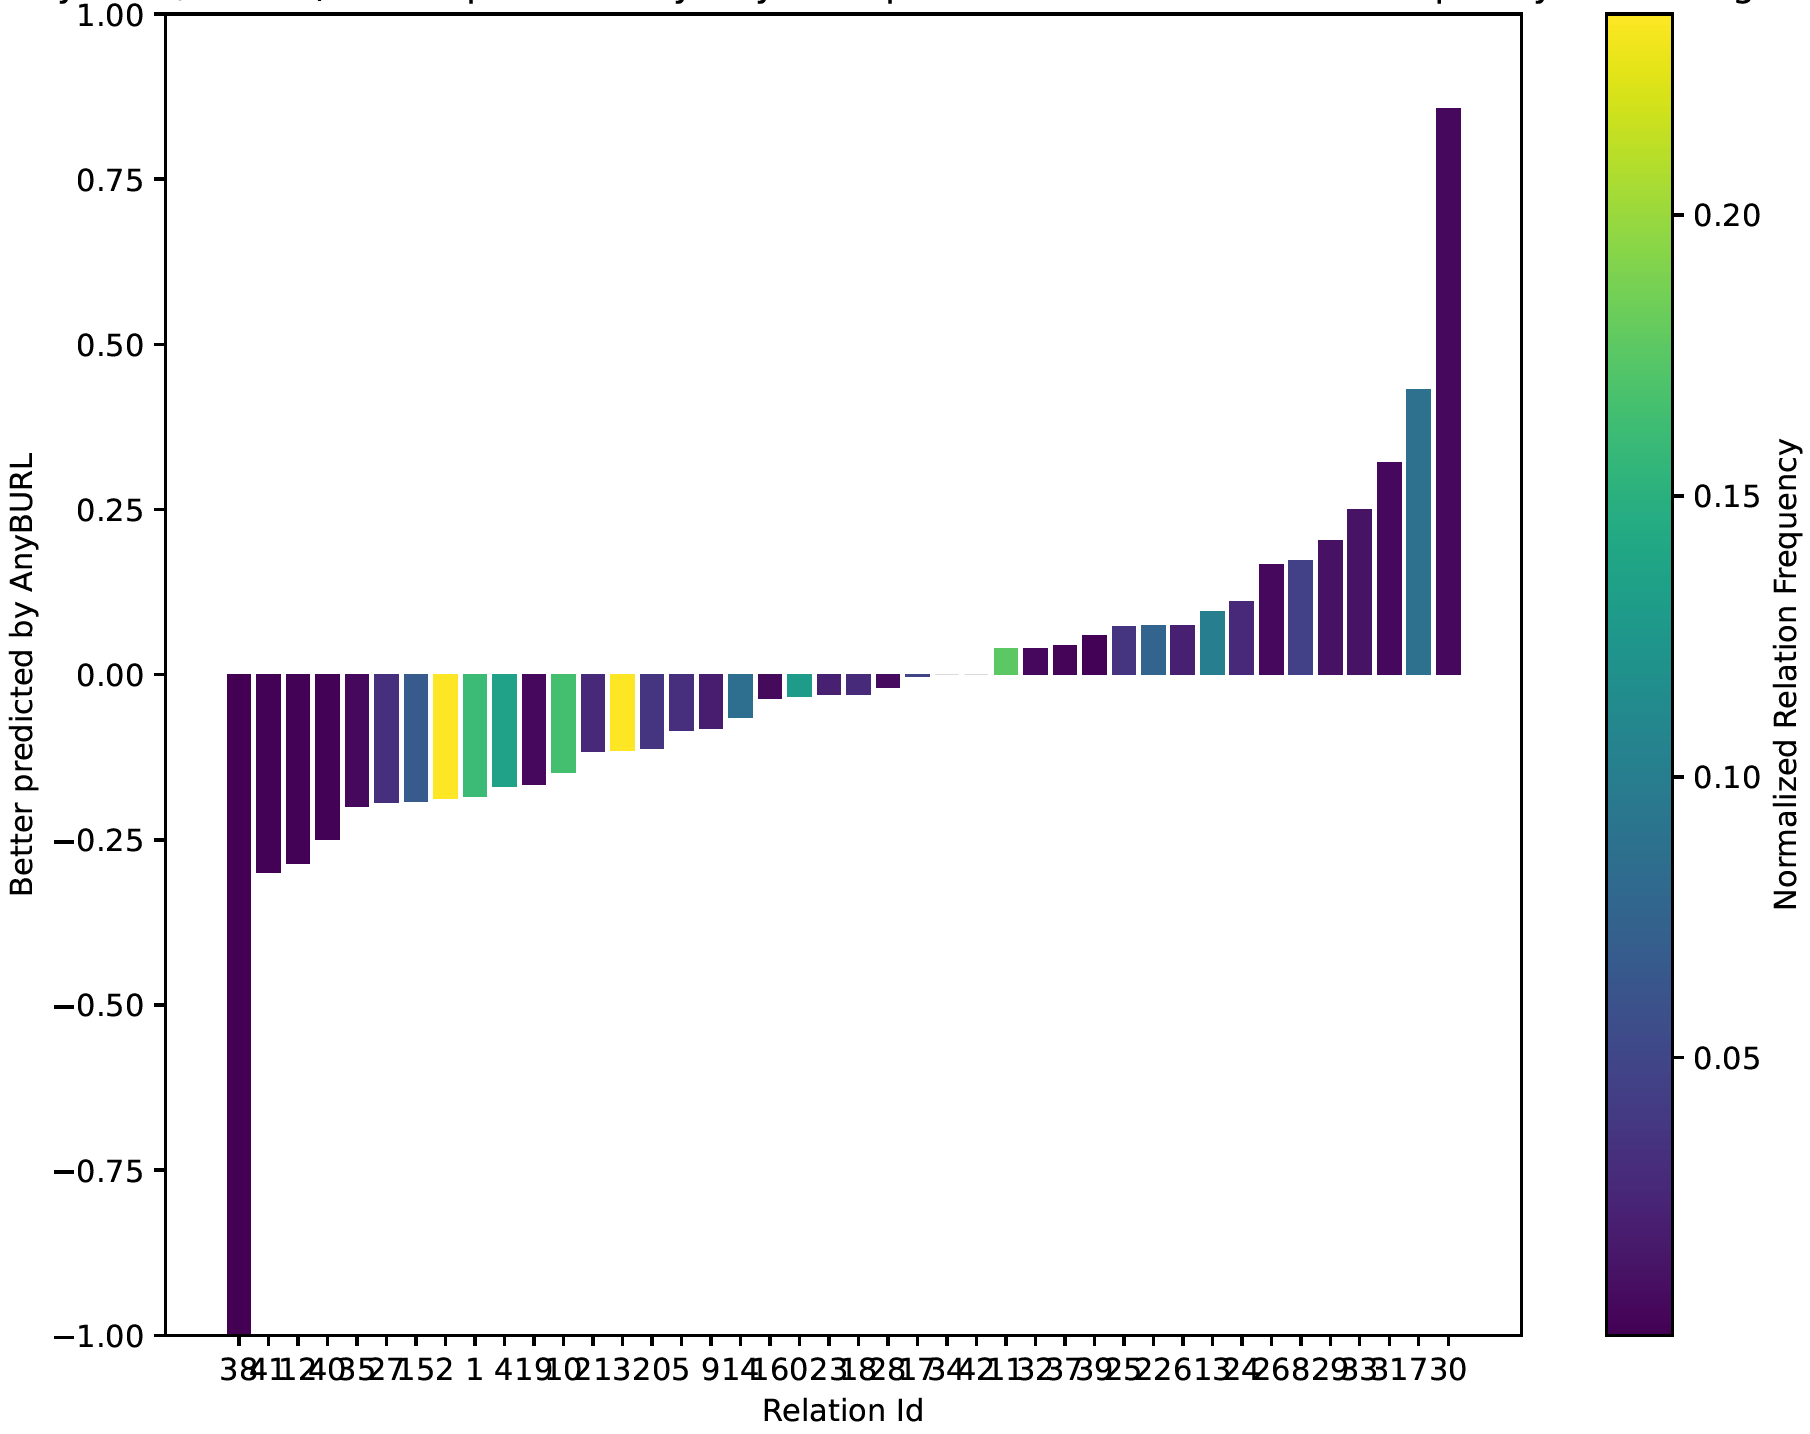
\includegraphics[width=0.45\textwidth]{images/relation_freq_anyburl_conve_codex.PNG}
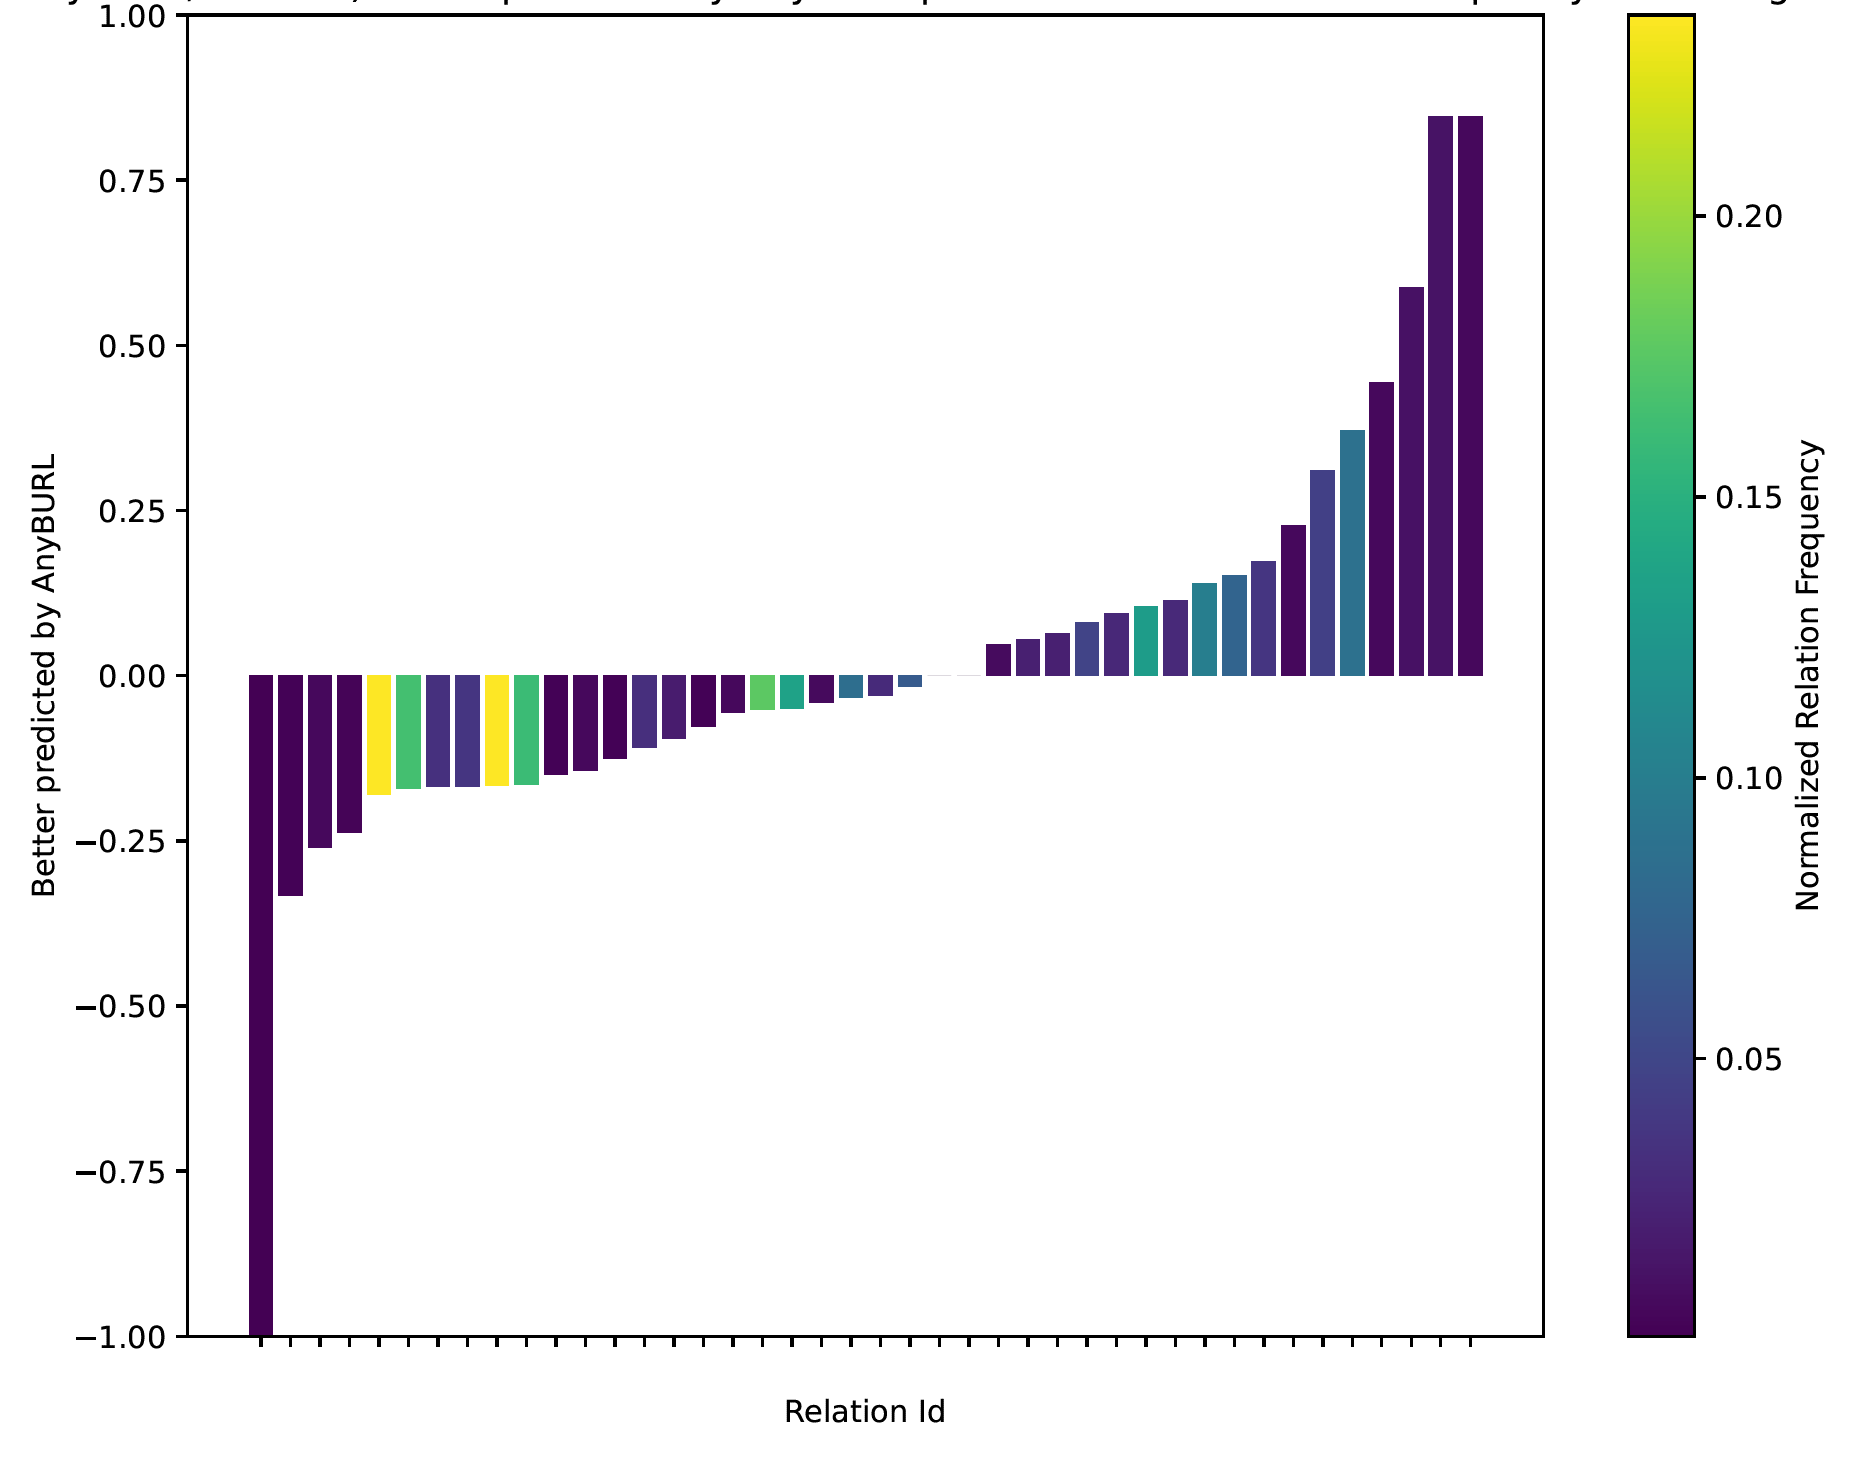
\includegraphics[width=0.45\textwidth]{images/relation_freq_anyburl_rescal_codex.PNG}
\caption{Comparison of AnyBURL and ConvE (left) RESCAL (right) on CoDEx-M in regard to the relation frequency}
\label{fig:relation_freq_anyburl_conve_rescal_codex}
\end{figure}

On FB15k-237 we can make similar observations. Figure \ref{fig:relation_freq_anyburl_complex_fb15k} compares AnyBURL and ComplEx. Most frequent relations are in average all better predicted by ComplEx but only with the average being close to $-0.25$ which again indicates that there is no strong correlation but that there might possibly be a weaker connection between the relation frequency and the performance of the approaches. The same comparison on FB15k-237 with ConvE and RESCAL produces similar results as can be seen in appendix \ref{appendix:relation_freq_fb15k}.

\begin{figure}[H]
\centering
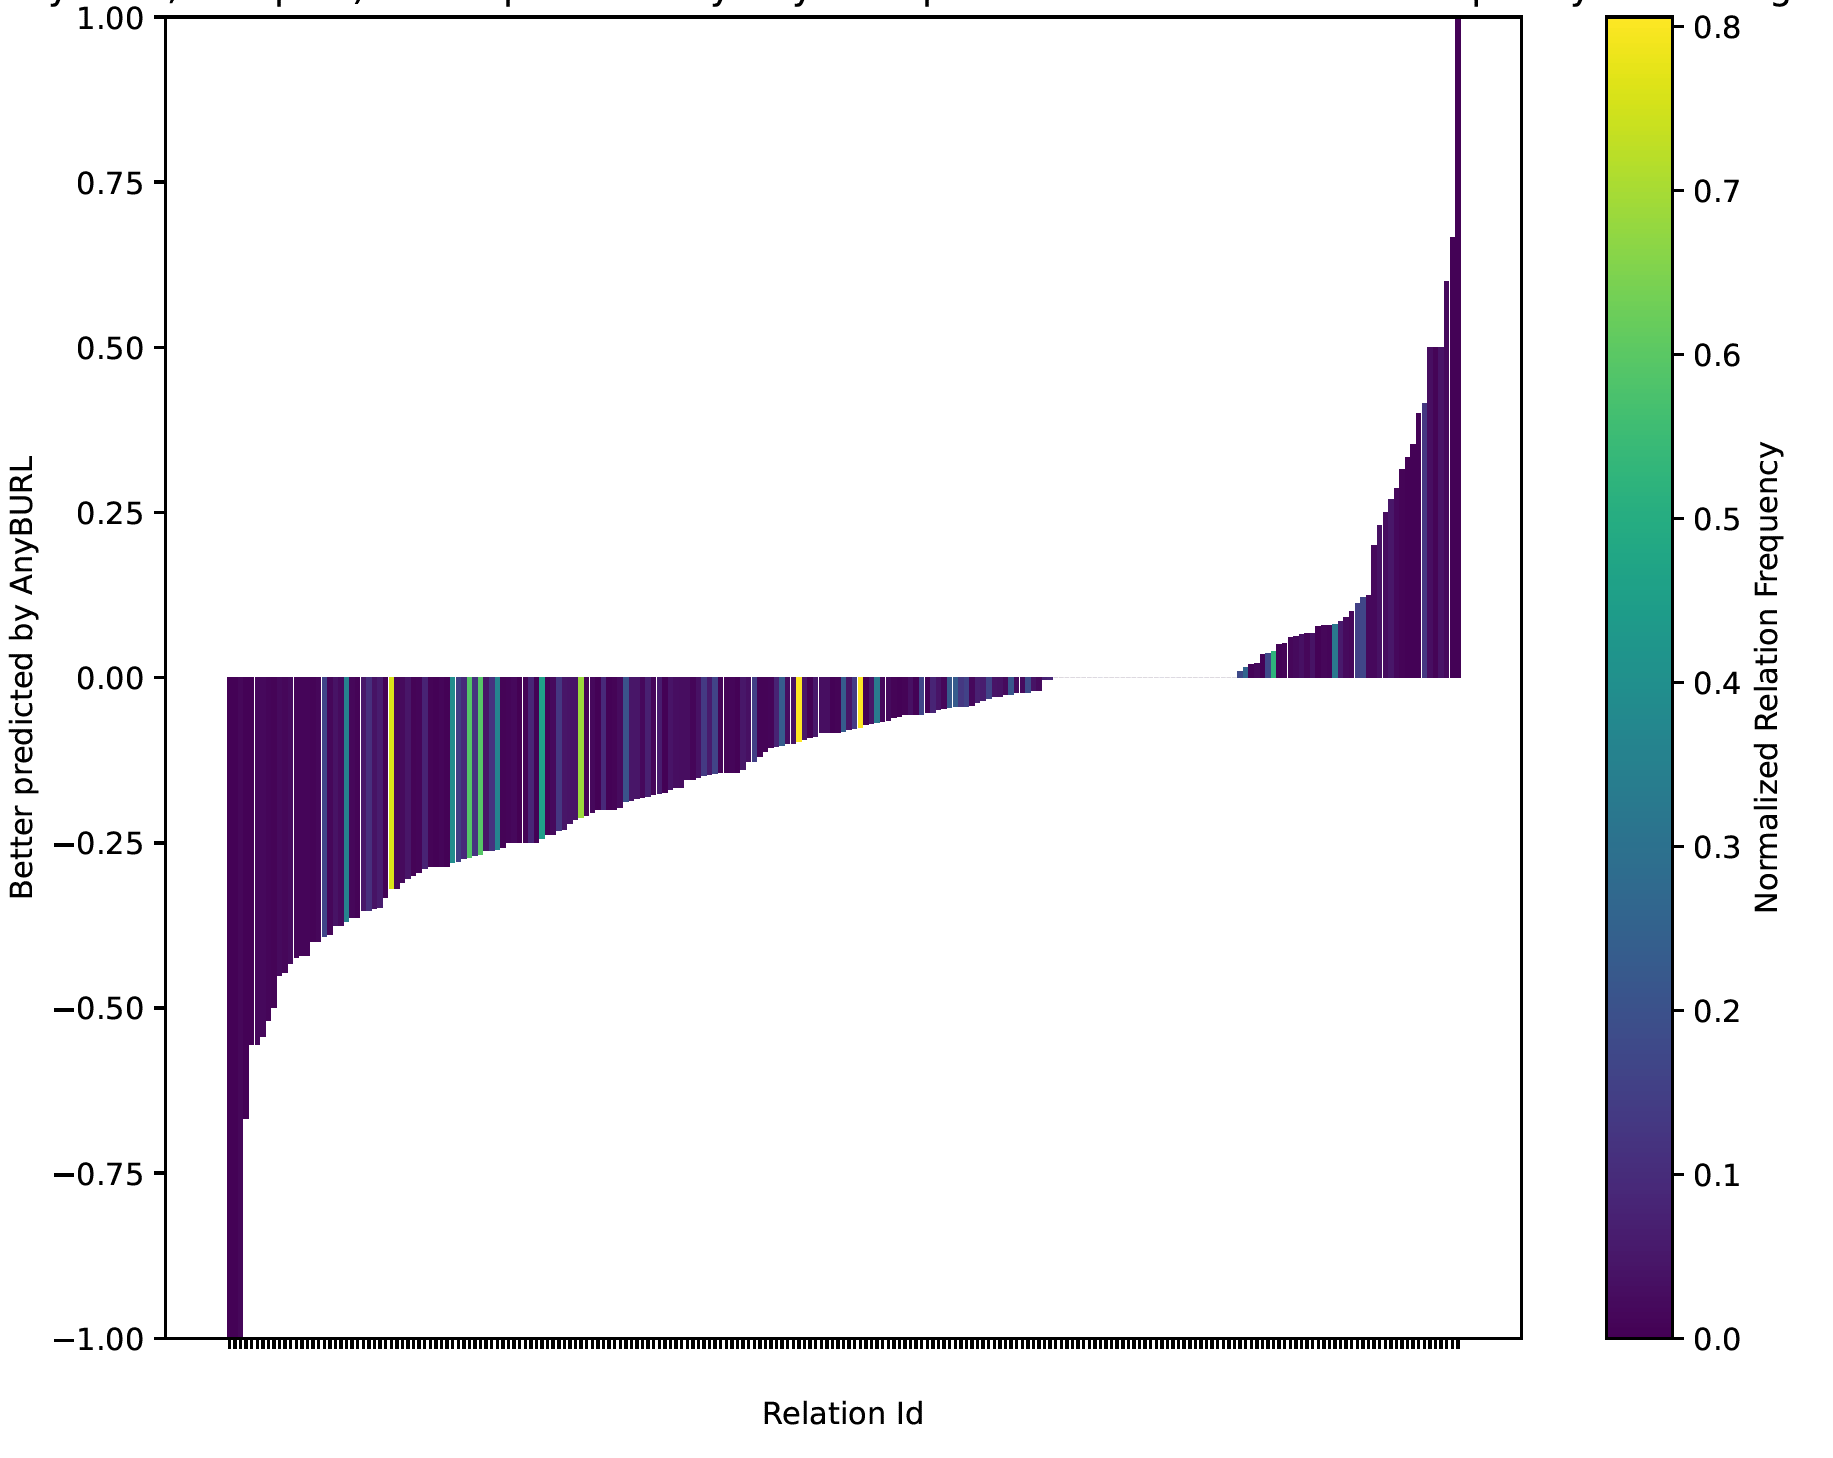
\includegraphics[width=0.9\textwidth]{images/relation_freq_anyburl_complex_fb15k.PNG}
\caption{Comparison of AnyBURL and ComplEx on FB15k-237 in regard to the relation frequency}
\label{fig:relation_freq_anyburl_complex_fb15k}
\end{figure}

On YAGO3-10 two relations dominate in occurrence all others. In figure \ref{fig:relation_freq_yago} we see that the second and third relation occur both more than $300000$ times in the trainings data while the next frequent relation occurs less than $100000$ times and the ones after that significantly less often. 

Figure \ref{fig:relation_freq_anyburl_complex_yago} shows us that both of these relations are better predicted by ComplEx but the average $better\_predicted\_by$ value is so close to $0$ that it can not be argued that ComplEx predicts relations frequently occurring in the trainings data better than AnyBURL on YAGO3-10.

\begin{figure}[H]
\centering
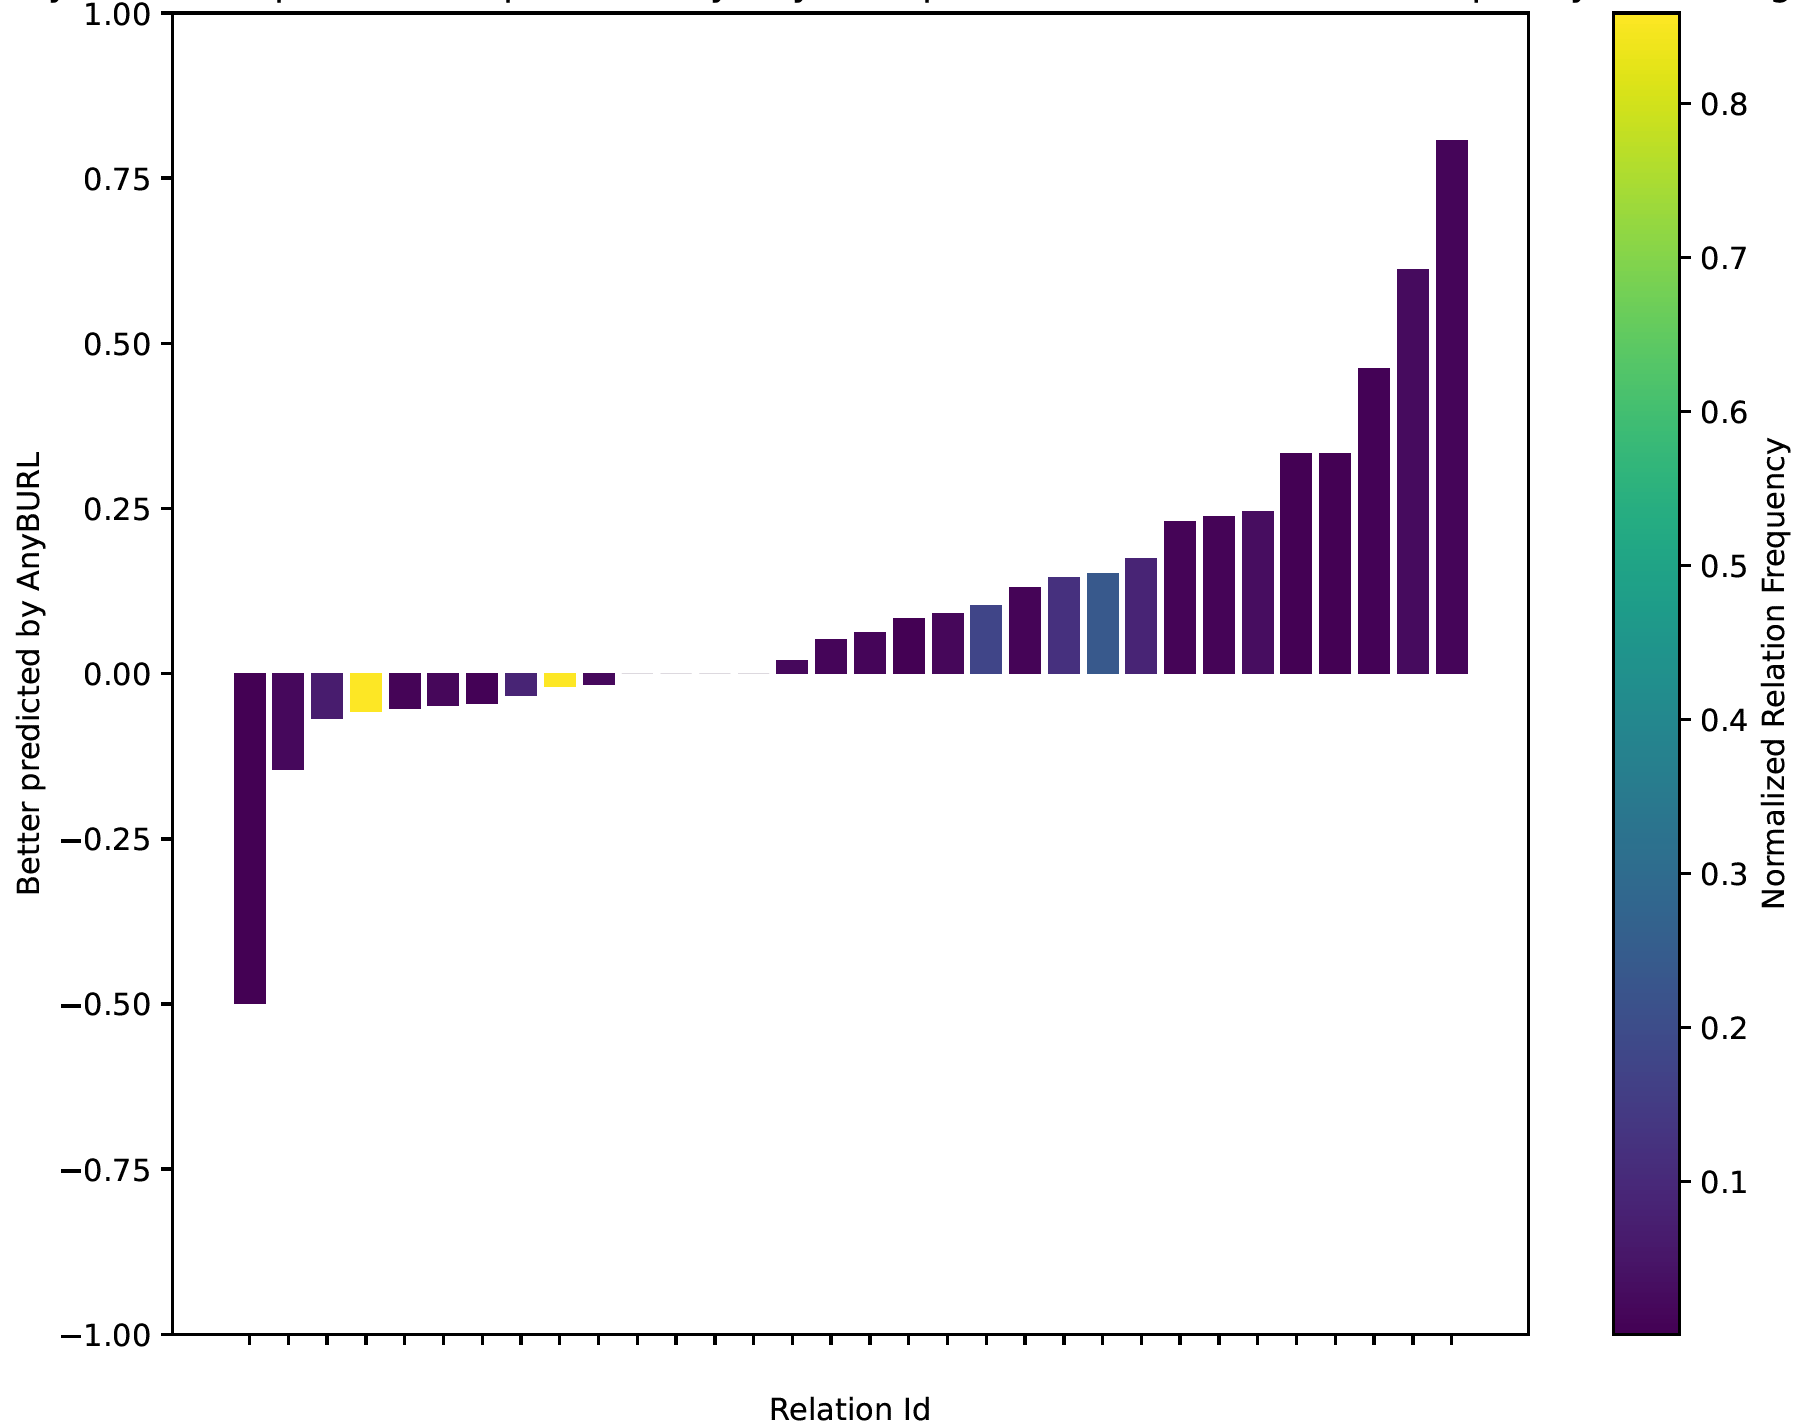
\includegraphics[width=0.9\textwidth]{images/relation_freq_anyburl_complex_yago.PNG}
\caption{Comparison of AnyBURL and ComplEx on YAGO3-10 in regard to the relation frequency}
\label{fig:relation_freq_anyburl_complex_yago}
\end{figure}

To sum up the results in regard to the relation frequency, we have now seen that on CoDEx-M and FB15k-237 triples with frequent relations tend towards being better predicted by the embedding-based models compared to AnyBURL. But this tendency is only small and furthermore this observation can not be made on YAGO3-10.

\subsection{Entity Frequency in Trainings Data}
Similar to the relations the entities are also not equally often represented in the datasets. For CoDEx-M we can see the entity distribution of the trainings data in figure \ref{fig:entity_freq_codex} and for the other dataset in appendix \ref{appendix:entity_freq}. 

Therefore I also wanted to investigate whether the frequency of the entities in the trainings data influences which approach performs better. 

\begin{figure}[H]
\centering
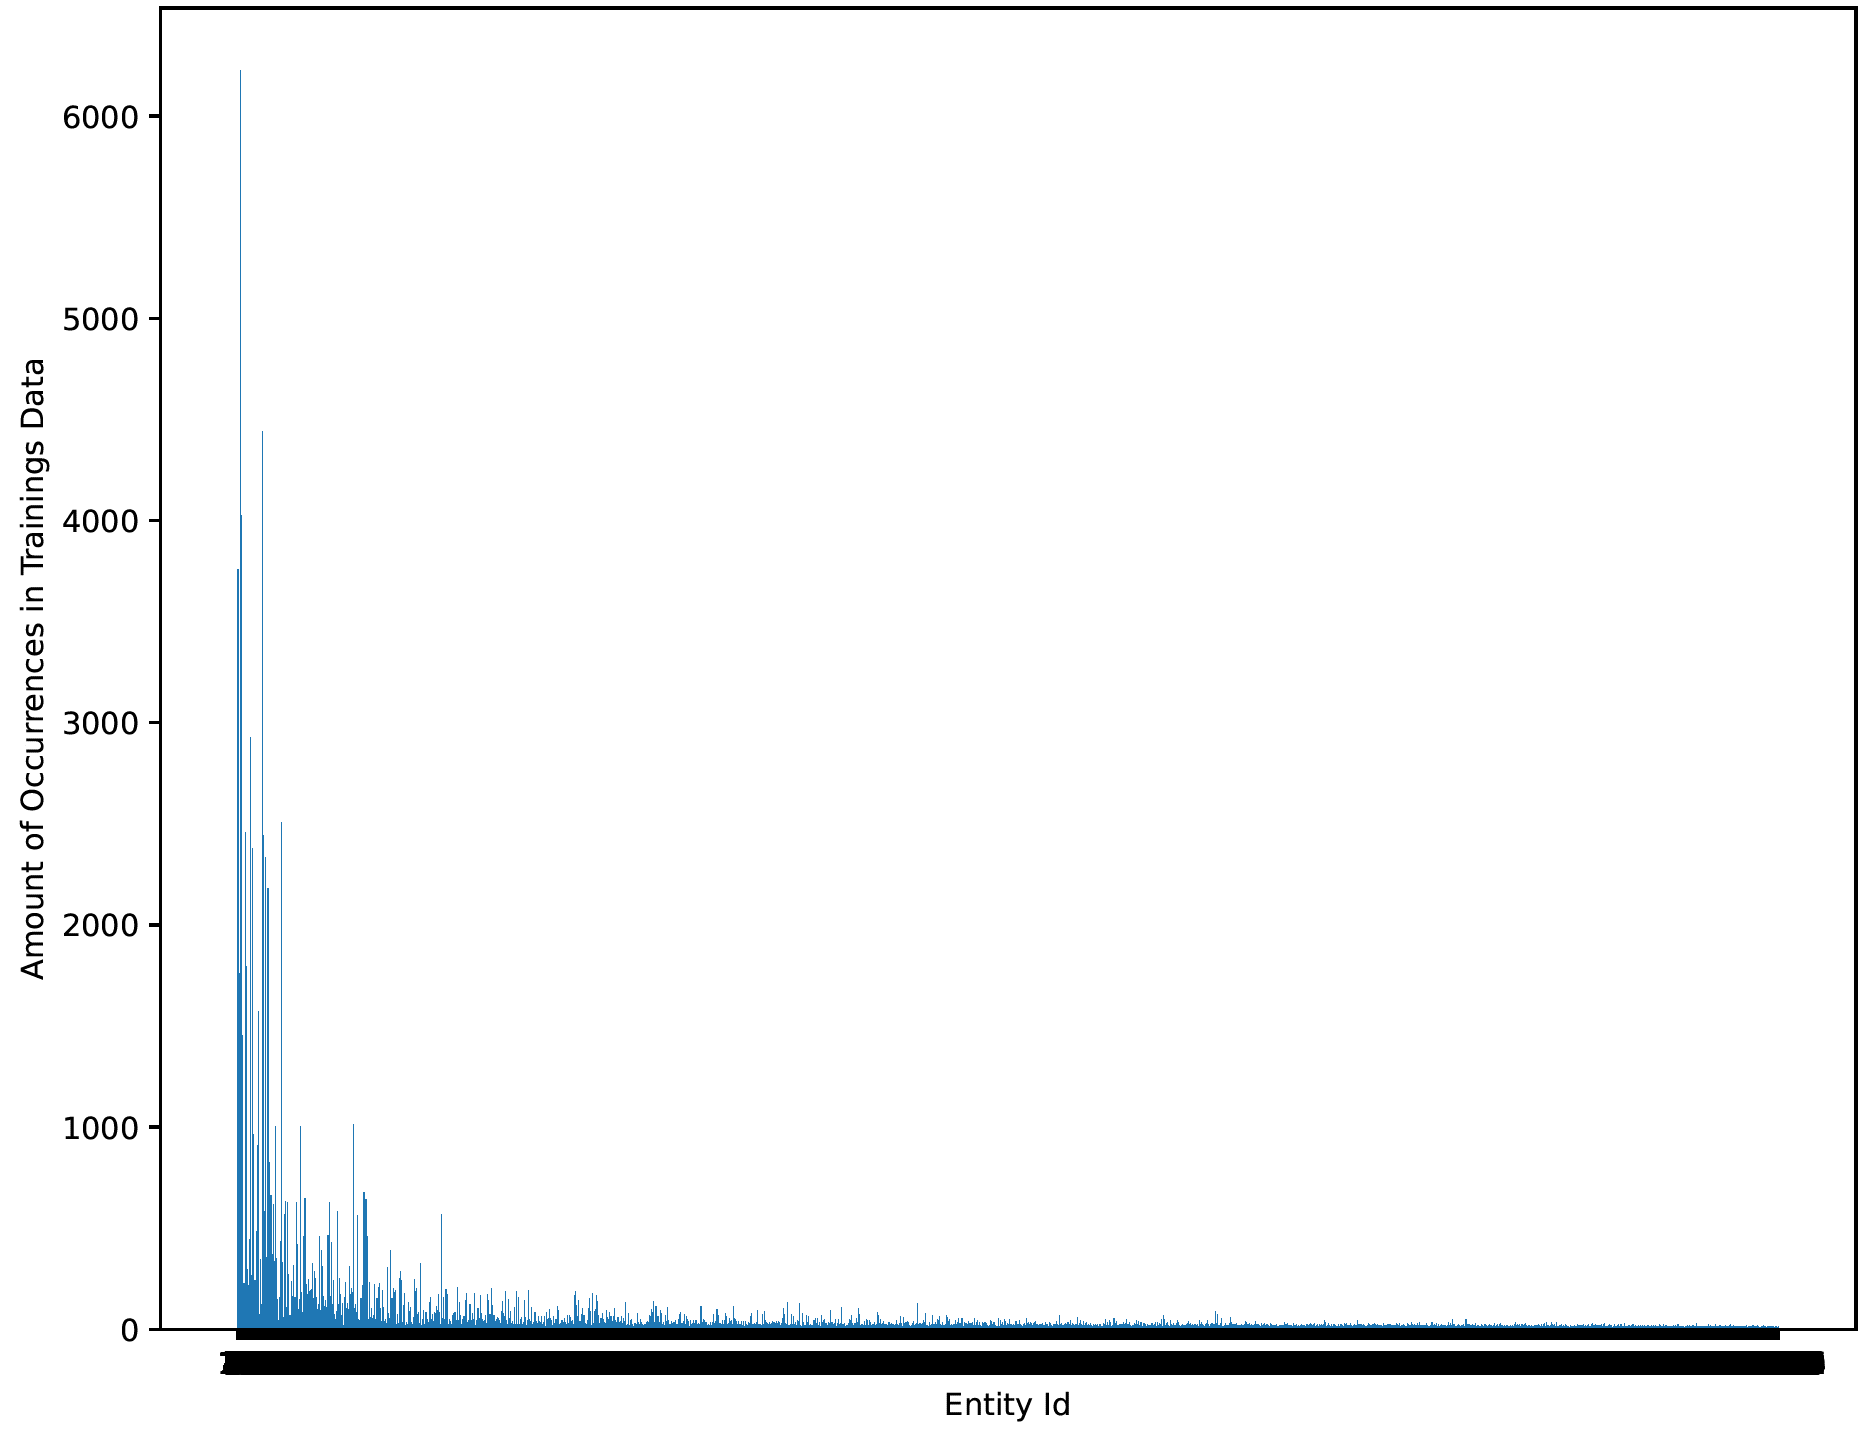
\includegraphics[width=0.9\textwidth]{images/entity_freq_codex.PNG}
\caption{Entity frequency in trainings data for CoDEx-M}
\label{fig:entity_freq_codex}
\end{figure}

Different than when making the comparison in regard to relation frequency is that for the entity frequency there are always two values one frequency value for the head and one for the tail. In first attempts at creating this comparison I simply used either of these value and created one graph for each. Since the triples are predicted in both directions, the head/ tail is sometimes a part of the question and sometimes the answer. Therefore I found that it makes more sense to rephrase the question and ask whether the frequency of the question entity or the frequency of the answer entity influences which approach performs better. The question entity here is in case the tail is predicted the head and in case the head is predicted the tail. For the answer entity it is the other way around.

Another problem for creating this comparison is the amount of unique entities the datasets contain. Plotting a bar for each entity and colouring it like it was done for the relation frequency would result in an incomprehensible mess. Therefore I created ten normalized frequency bins in steps of $0.1$ and calculated the average $better\_predicted\_by$ value for each bin. 

Figure \ref{fig:entity_question_tail_anyburl_complex_codex} plots this average and overlays the question entity frequency. Most of the bins average $better\_predicted\_by$ values are close to $0$ with the only outliers being the $(0.7, 0.8]$ and $(0.5, 0.6]$ bins. These two slightly tend towards being better predicted by AnyBURL. But since the bins above these all tend towards ComplEx I would not say that this shows any pattern.

\begin{figure}[H]
\centering
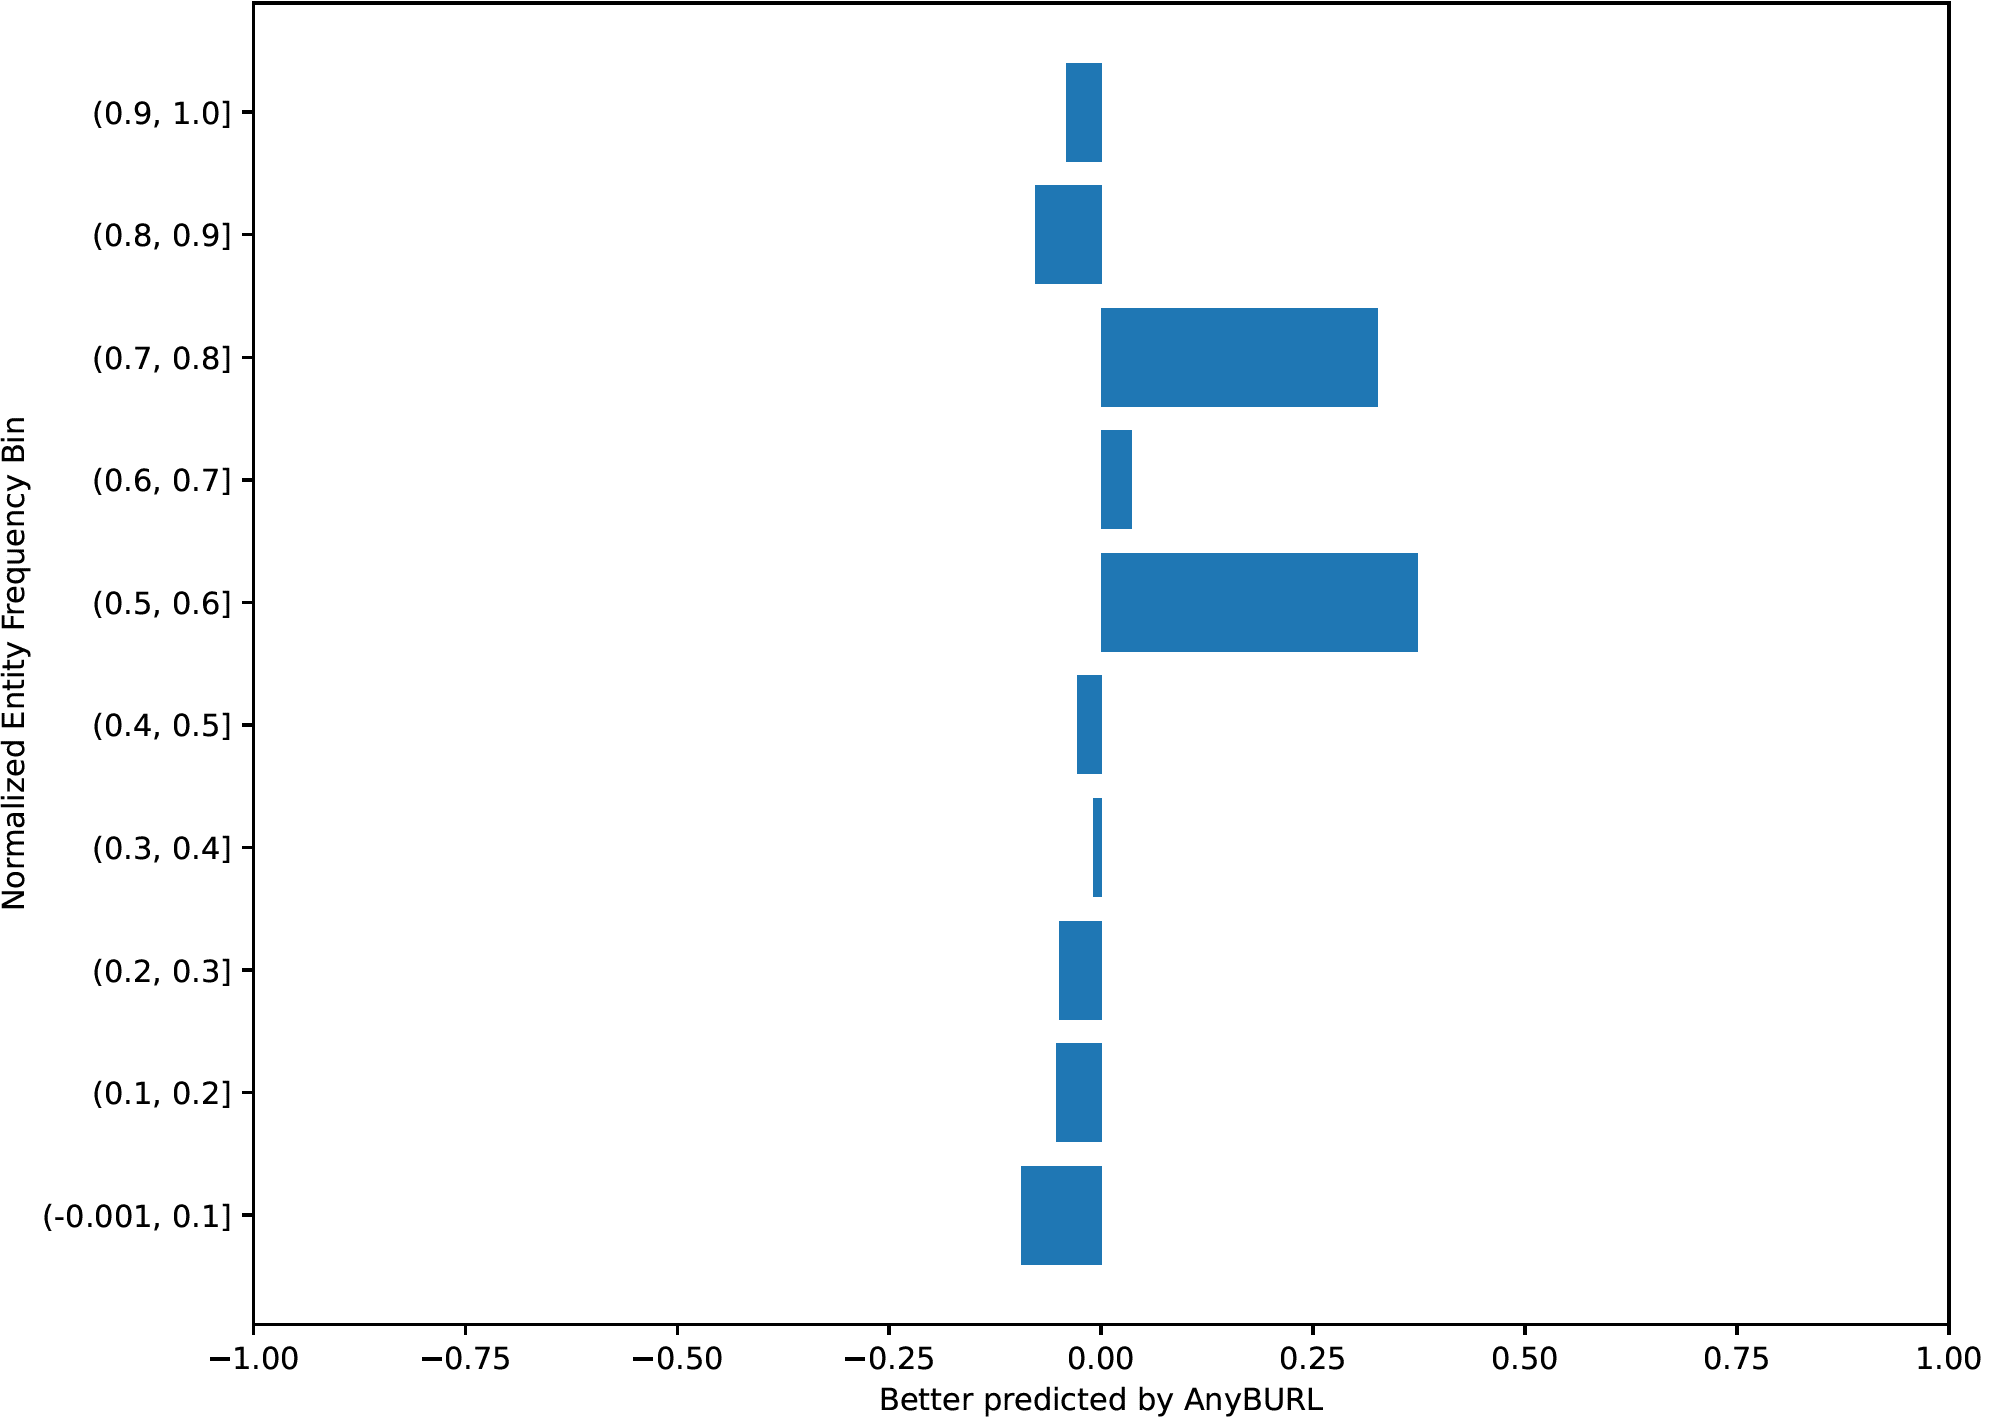
\includegraphics[width=0.9\textwidth]{images/entity_freq_question_anyburl_complex_codex.PNG}
\caption{Comparison of AnyBURL and ComplEx on CodEx-M in regard to the question entity frequency}
\label{fig:entity_question_tail_anyburl_complex_codex}
\end{figure}

When plotting the same figure for the frequency of the answer entity, as can be seen in figure \ref{fig:entity_answer_tail_anyburl_complex_codex}, we notice that all bins above $0.4$ tend towards AnyBURL, while all below tend towards ComplEx. While this shows a slight tendency since the values are quiet low I would argue that this also does not express a clear pattern. 

\begin{figure}[H]
\centering
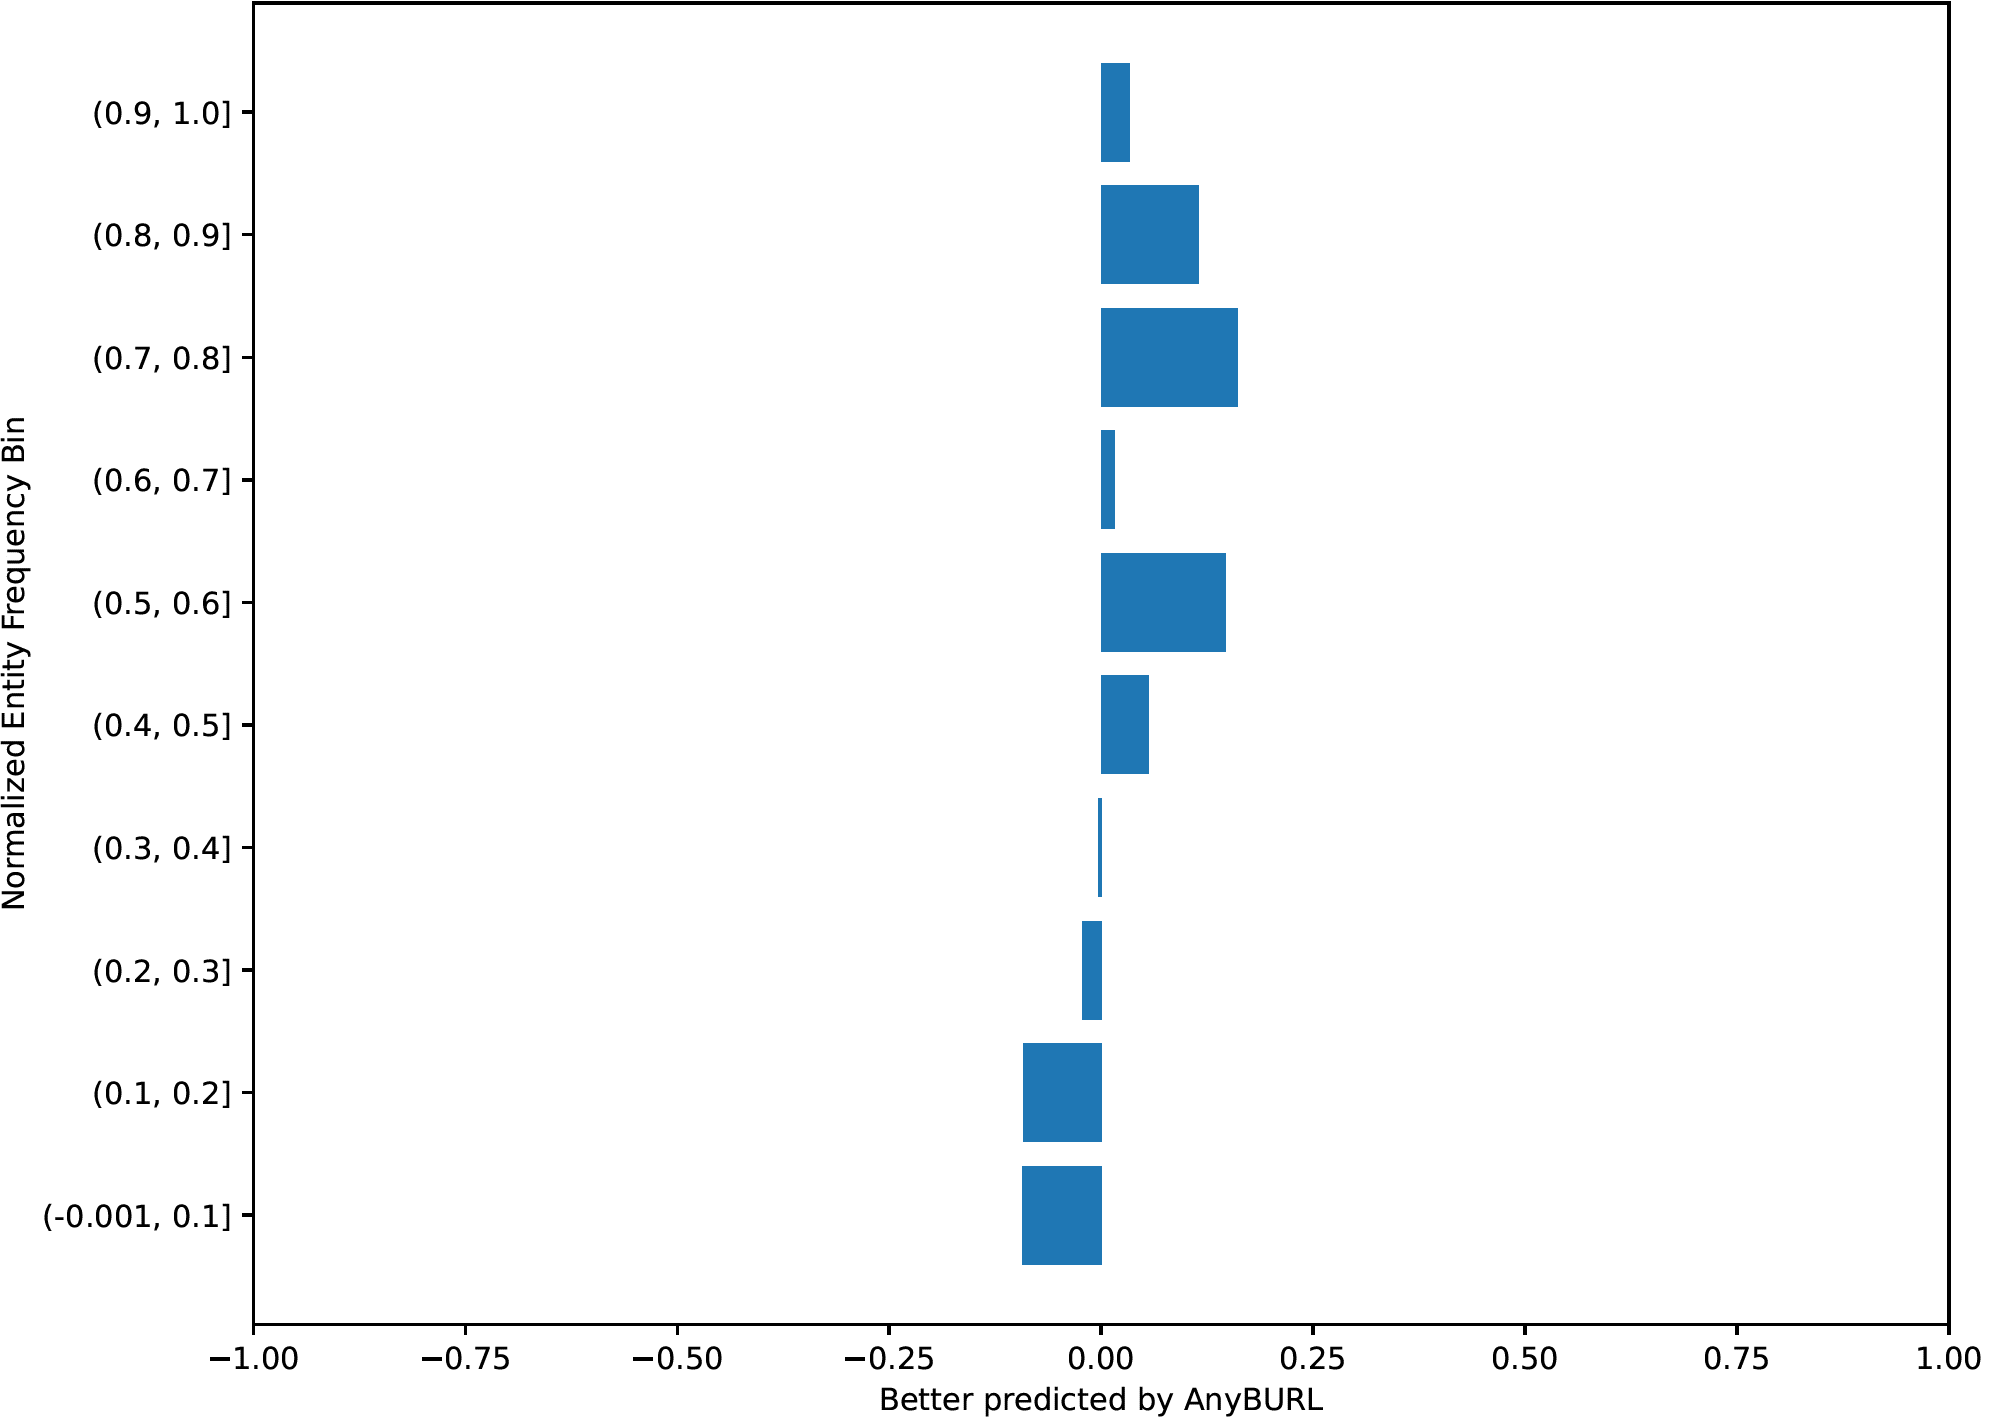
\includegraphics[width=0.9\textwidth]{images/entity_freq_answer_anyburl_complex_codex.PNG}
\caption{Comparison of AnyBURL and ComplEx on CodEx-M in regard to the answer entity frequency}
\label{fig:entity_answer_tail_anyburl_complex_codex}
\end{figure}

In appendix \ref{appendix:comparison_entity_freq} the same figures can be found for the other model-dataset combinations. All these also do not show a clear pattern, especially not one overarching different embedding-based models and/ or datasets. 

Even though I could not find a correlation between the model performances and the entity frequency, I still also wanted to test if it has an influence when all three parts of the triple are frequent. For that I added the two entity frequencies together and also included the relation frequency. I used the same bins as define before and the result of this can be seen in figure \ref{fig:combined_freq_anyburl_complex_codex}. While some bins tend towards either of the models there also is no clearly recognizable pattern. As can be seen in appendix \ref{appendix:comparison_entity_freq} the same holds for all other model-dataset combinations.

\begin{figure}[H]
\centering
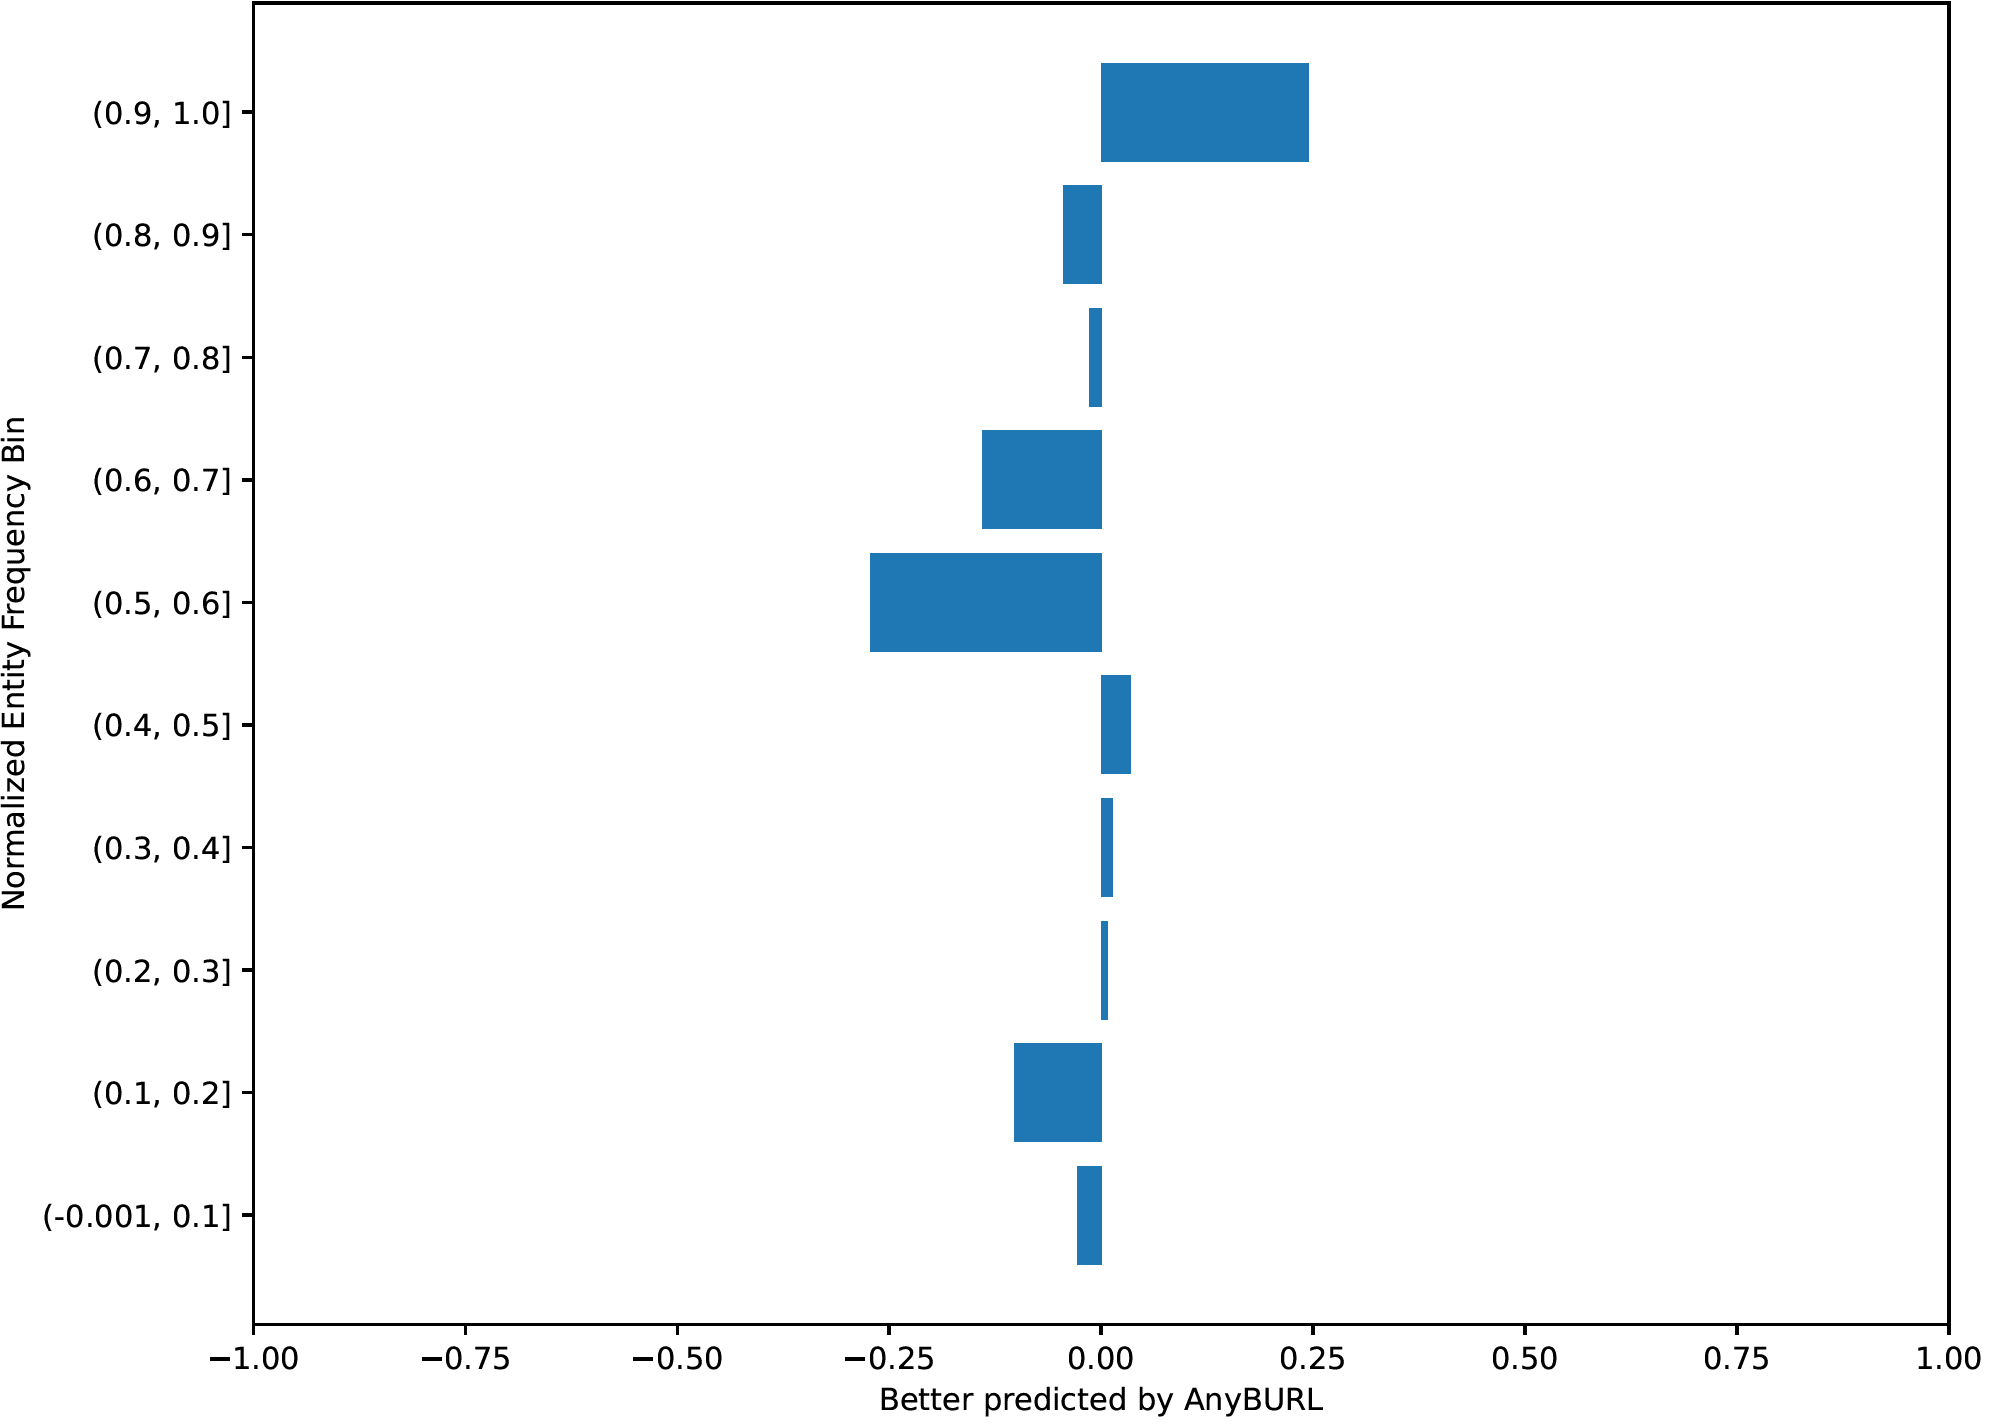
\includegraphics[width=0.9\textwidth]{images/combined_freq_anyburl_complex_codex.PNG}
\caption{Comparison of AnyBURL and ComplEx on CodEx-M in regard to the combined entity and relation frequency}
\label{fig:combined_freq_anyburl_complex_codex}
\end{figure}

In this section I have now shown that I could not find any evidence that the frequency of the entities in the trainings data influences which approach predicts a triple better.

\subsection{Existence of Similar Triples in the Trainings Data}
\label{sec:similar_triple_exist}
Next up I wanted to investigate whether it is easier for one of the approaches to predict a triple if a similar triple already exists in the trainings dataset. 
For example if we have a test triple $(h,r,t)$, does the trainings data contain a similar triple $(h,r,t')$ when predicting the tail or $(h',r,t)$ when predicting the head with $h\neq h'$ and $t\neq t'$. 

To achieve that my code labels every triple from the test set with a binary variable expressing whether at least one similar triple exists or not. 

In figure \ref{fig:similar_triples_binary_anyburl_complex_codex} expresses this information and compares AnyBURL and ComplEx on CoDEx-M where the $better\_predicted\_by$ value is the average of all triples belonging to the same binary class. As we can see the value averages are low values indicating that both models are almost equally good at predicting triples with or without similar triples in the trainings data. Interesting here is that ComplEx is slightly better in predicting triples when there is a similar triple and AnyBURL is better when there is non. What makes this interesting is that, as we can see in figure \ref{fig:similar_triples_binary_anyburl_conve_rescal_codex}, ConvE and RESCAL create a similar result. 

\begin{figure}[H]
\centering
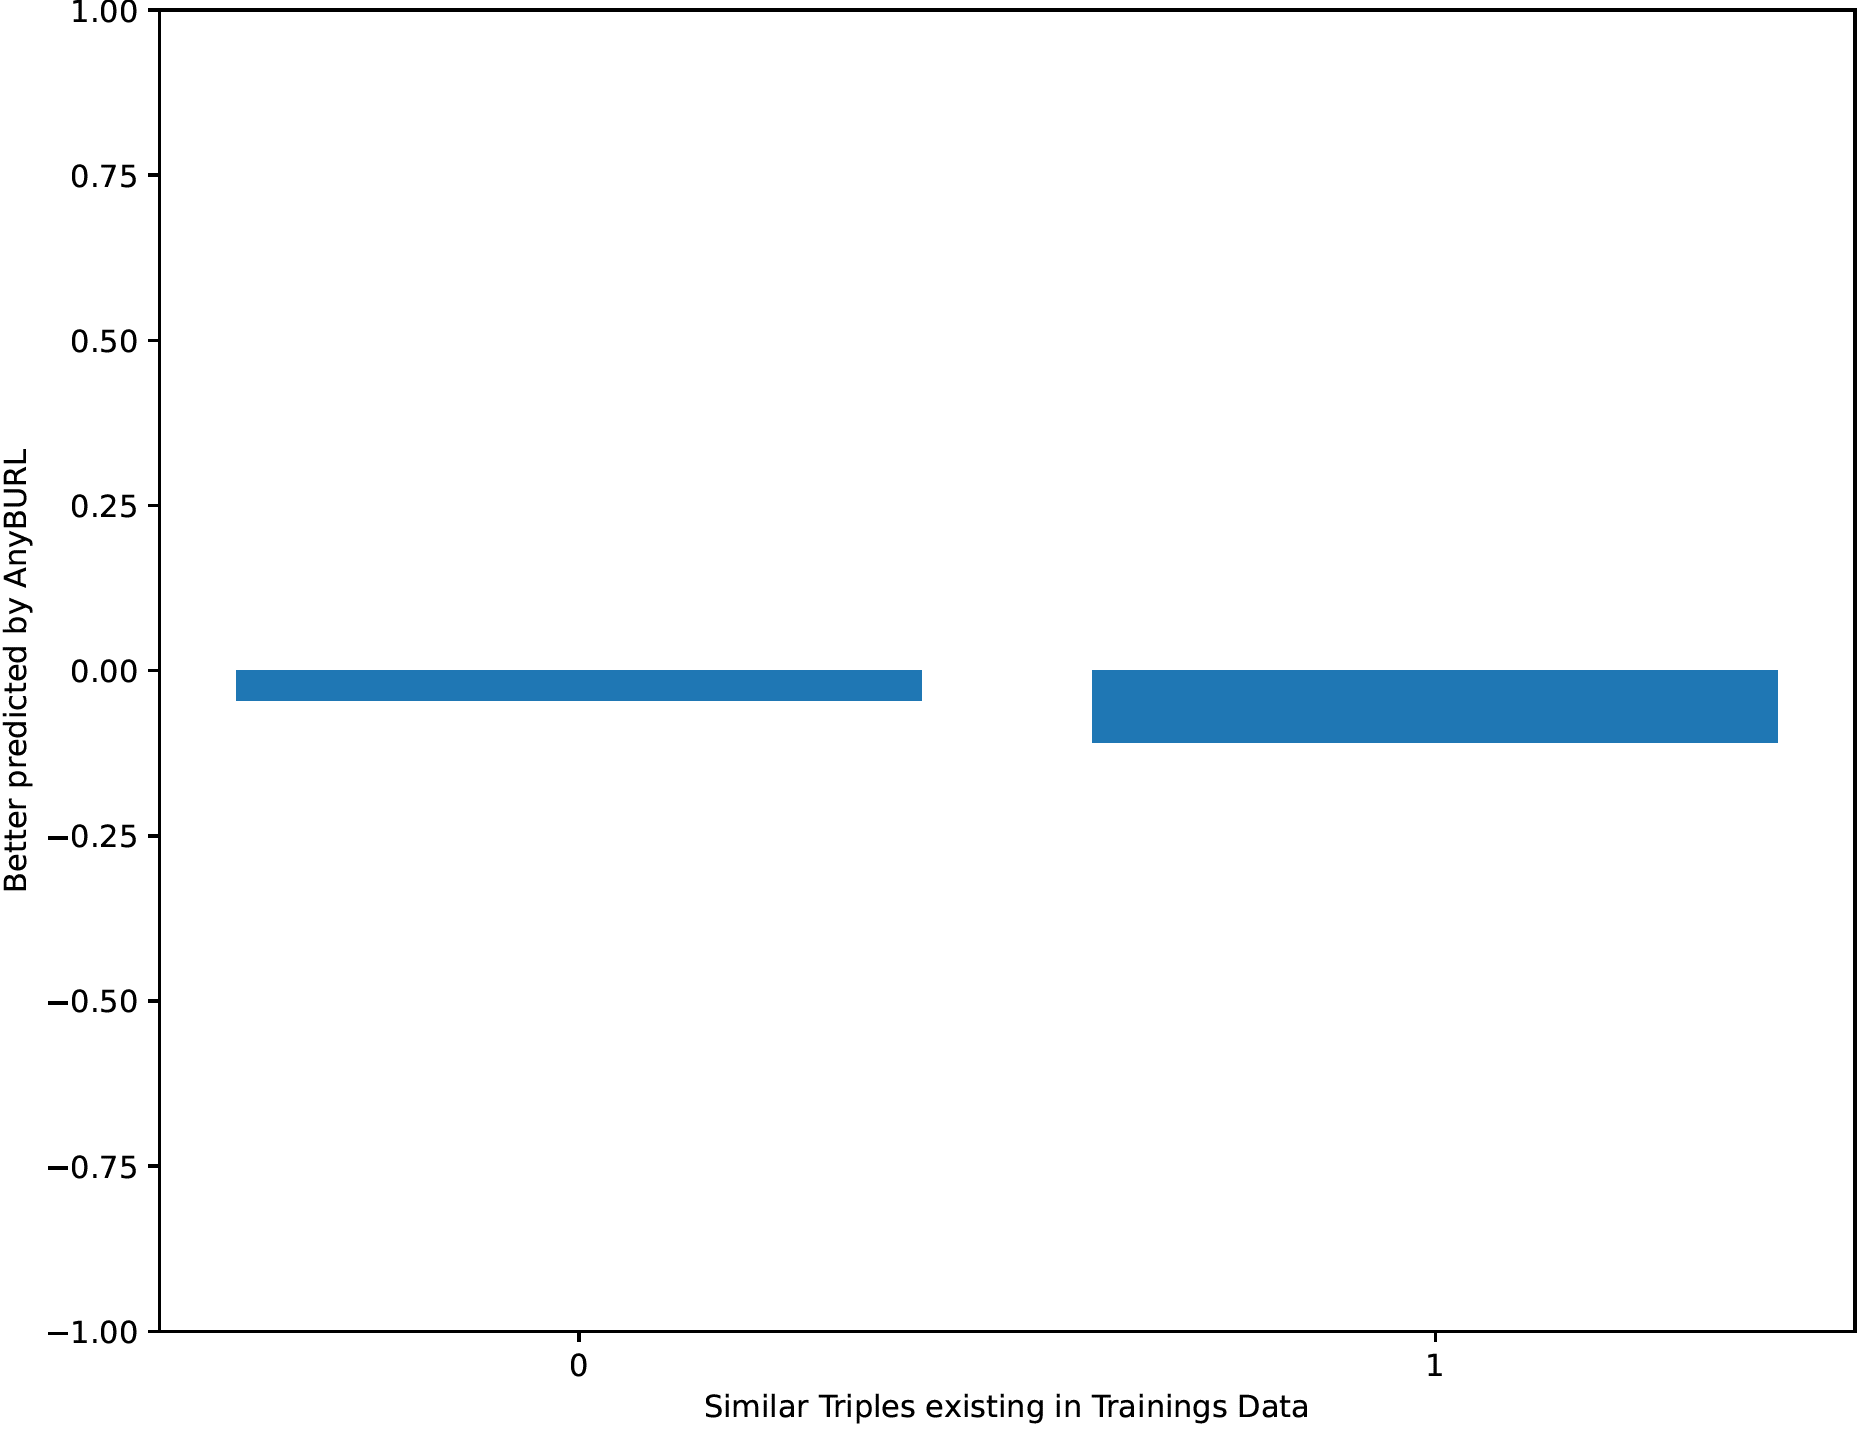
\includegraphics[width=0.9\textwidth]{images/similar_triples_binary_anyburl_complex_codex.PNG}
\caption{Comparison of AnyBURL and ComplEx on CodEx-M in regard to the existence of similar triples in the trainings data}
\label{fig:similar_triples_binary_anyburl_complex_codex}
\end{figure}

\begin{figure}[H]
\centering
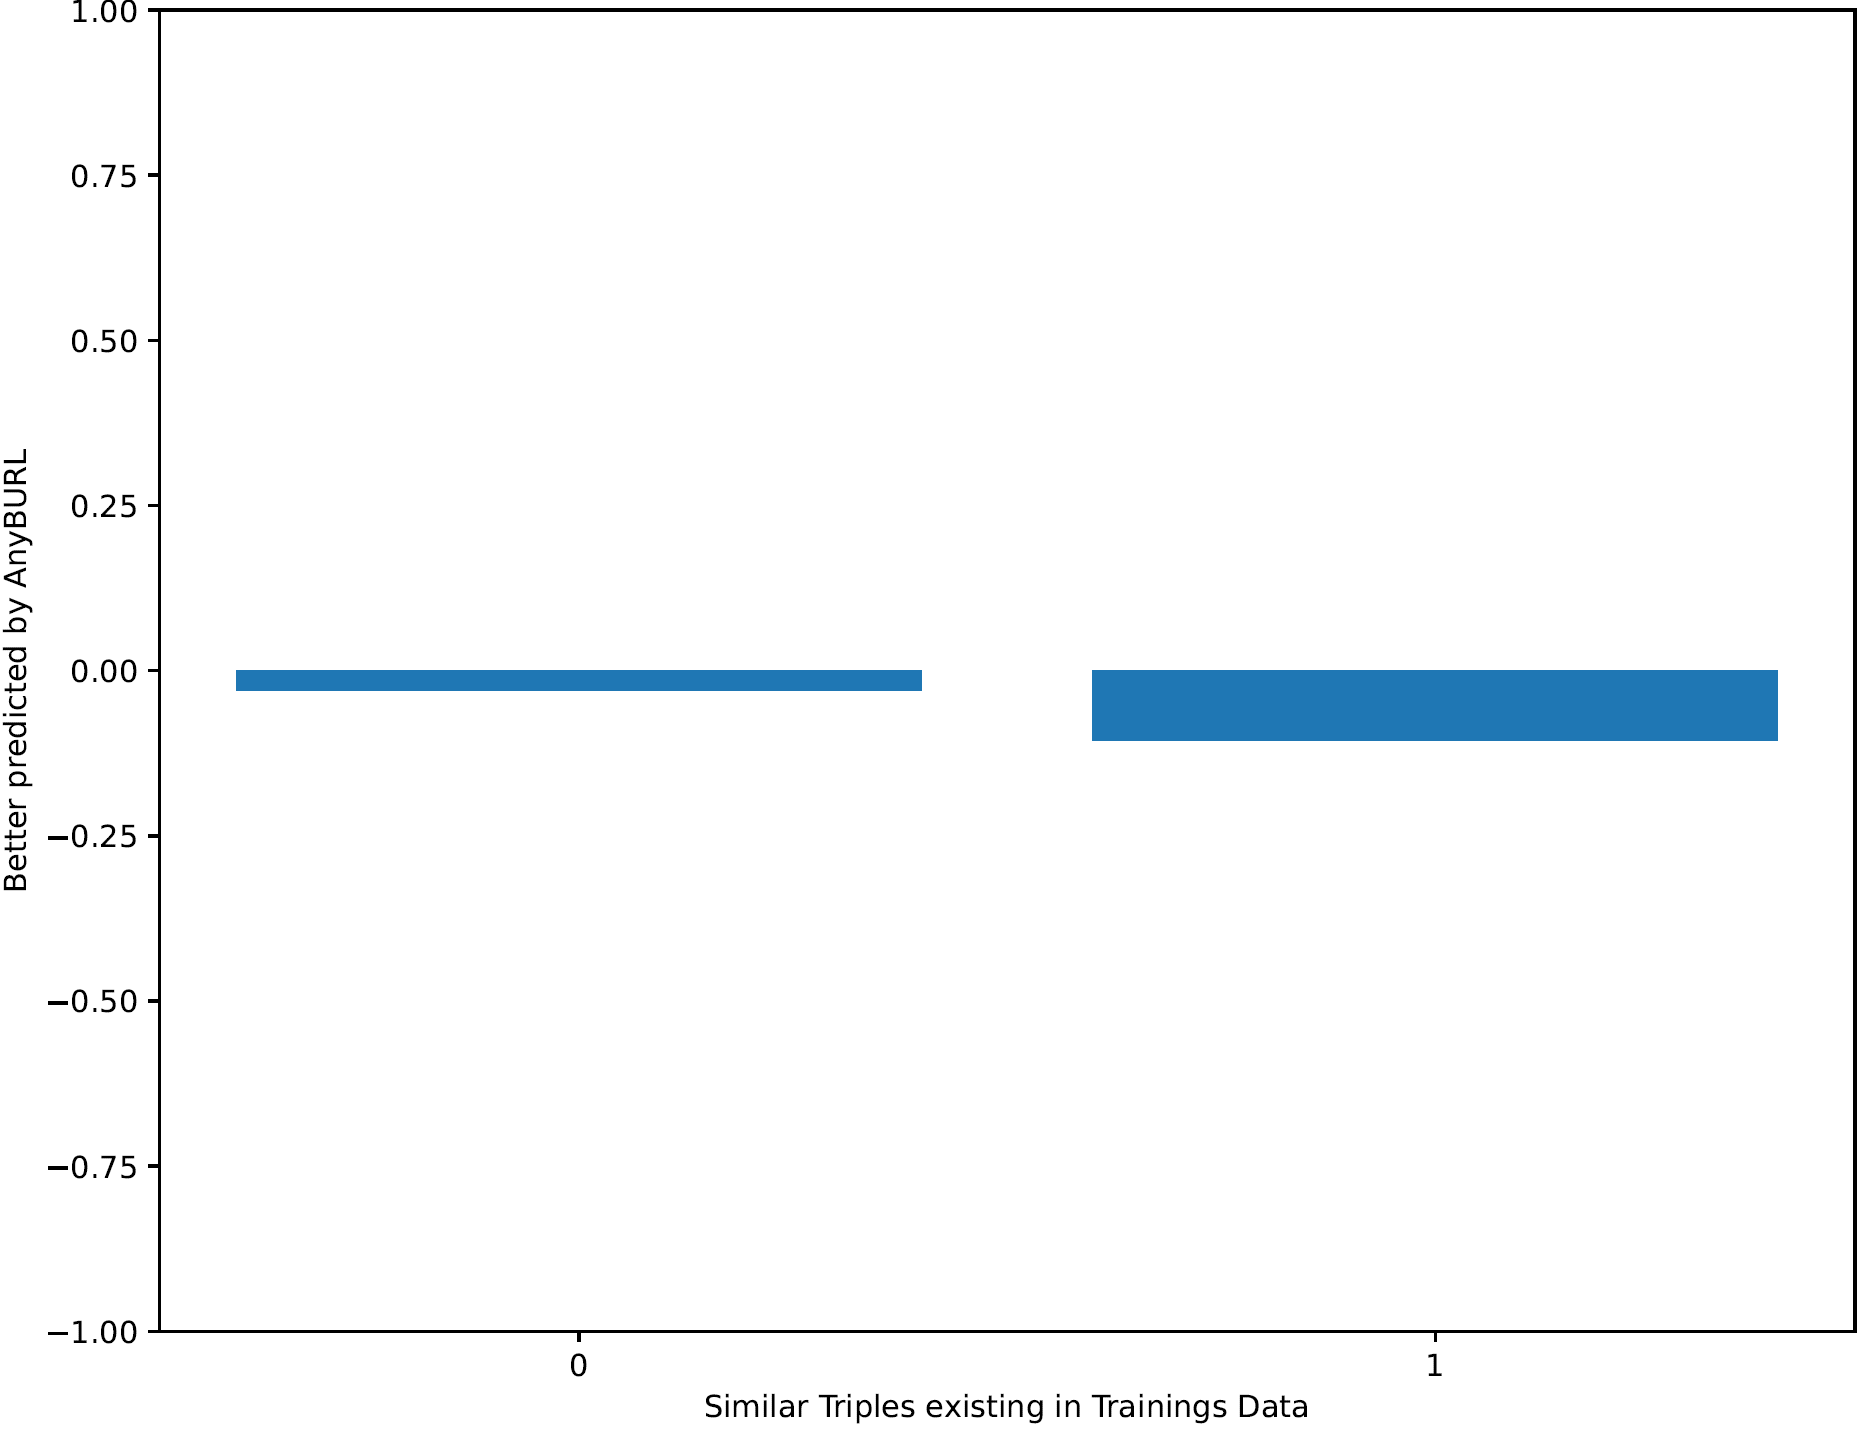
\includegraphics[width=0.45\textwidth]{images/similar_triples_binary_anyburl_conve_codex.PNG}
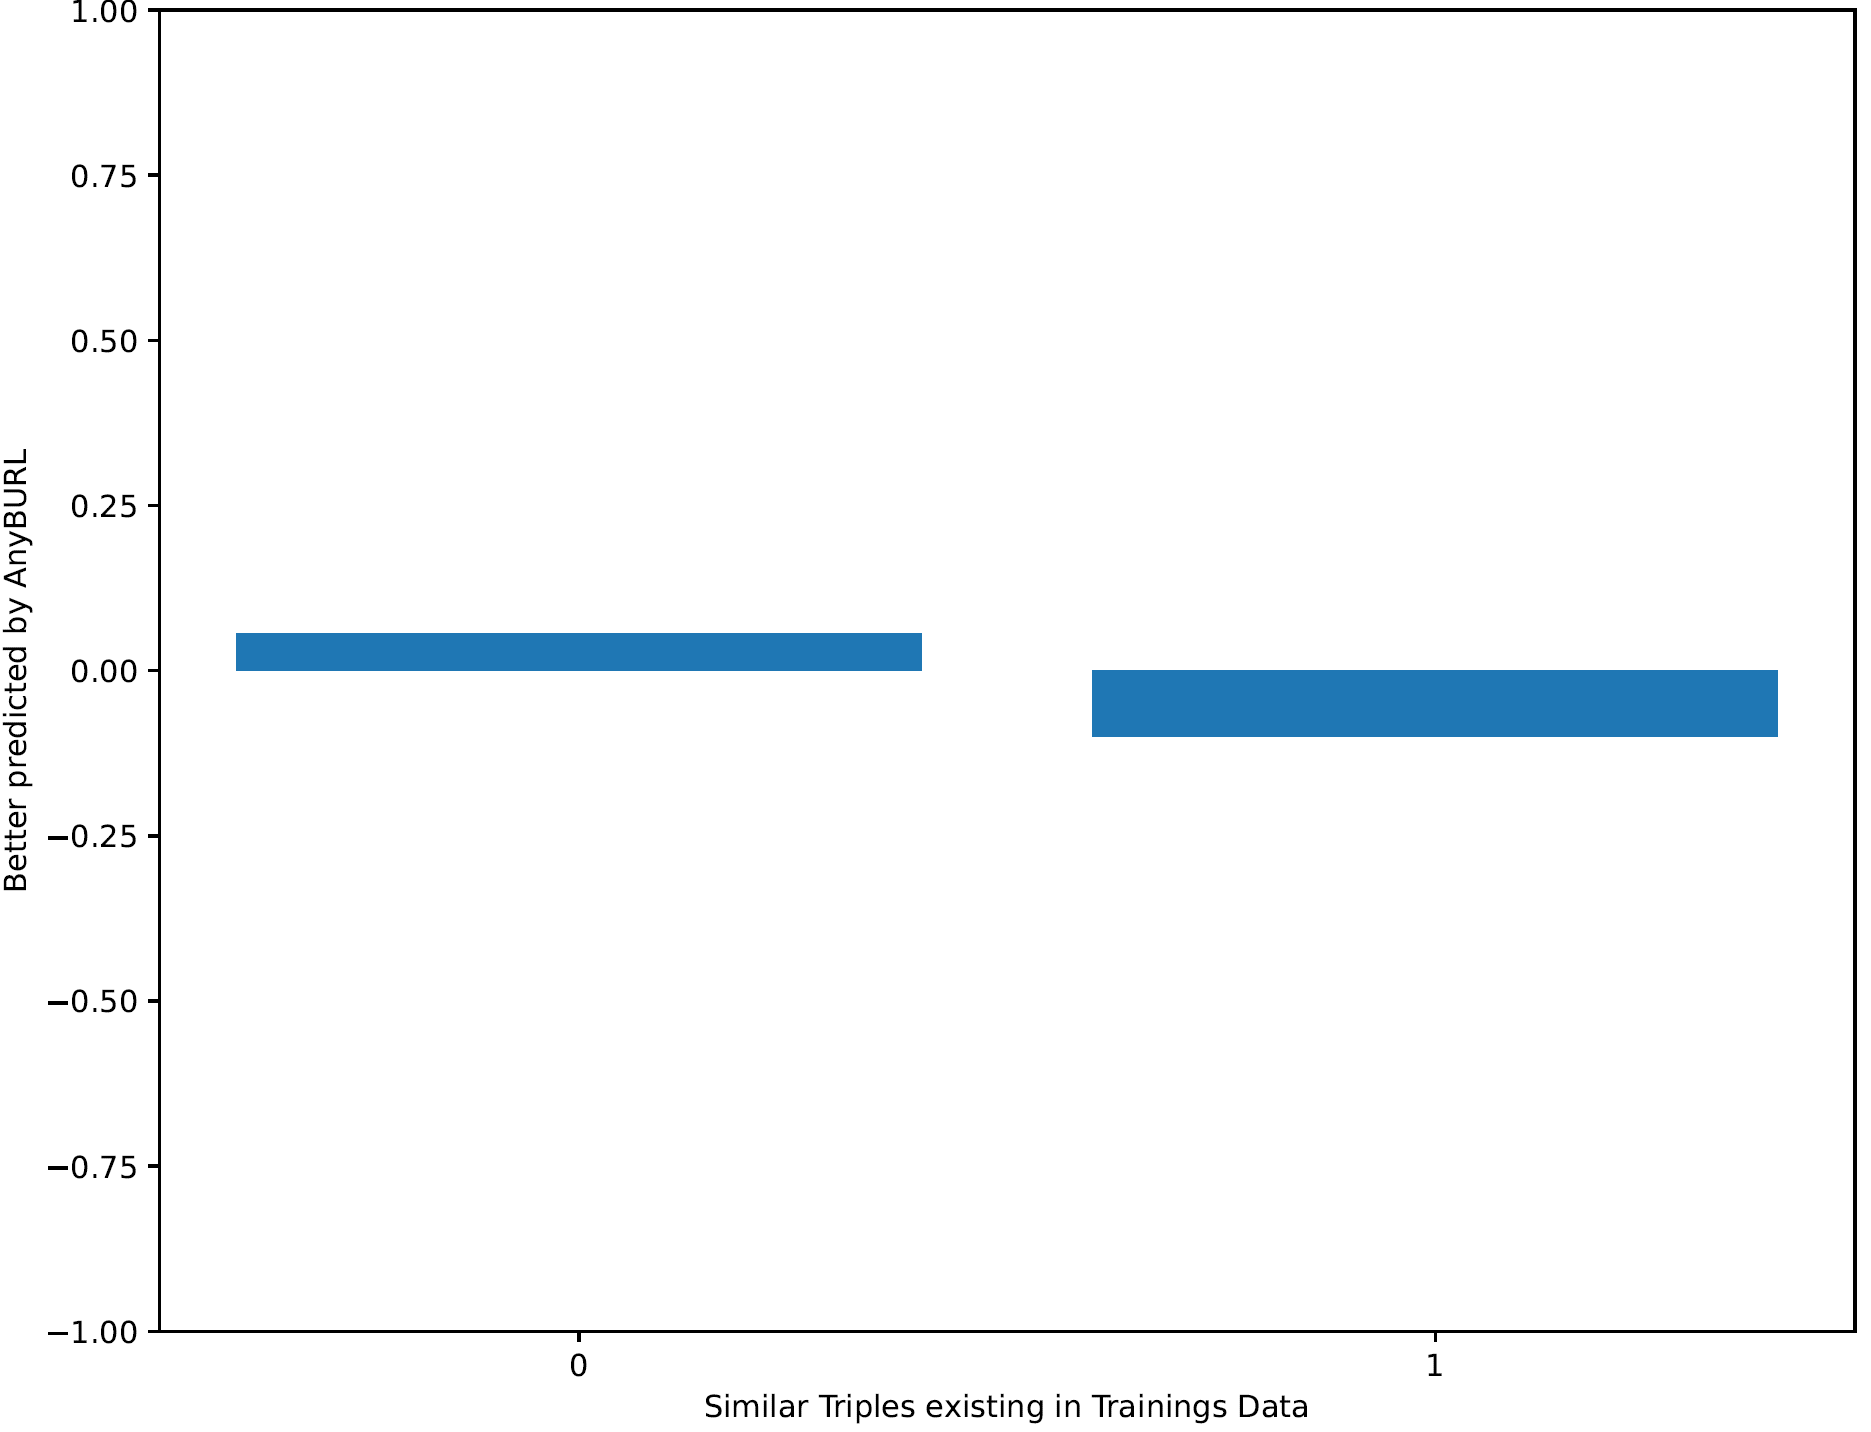
\includegraphics[width=0.45\textwidth]{images/similar_triples_binary_anyburl_rescal_codex.PNG}
\caption{Comparison of AnyBURL and ConvE (left) / RESCAL (right) on CodEx-M in regard to the existence of similar triples in the trainings data}
\label{fig:similar_triples_binary_anyburl_conve_rescal_codex}
\end{figure}

Plotting the same data for FB15k-237 and YAGO3-10 leads to comparable results. As can be seen in figure \ref{fig:similar_triples_binary_anyburl_complex_fb15k} comparing ComplEx and AnyBURL on FB15k-237 results in the same observations as before. Appendix \ref{appendix:similar_triples} shows that this also goes when comparing AnyBURL to ConvE and RESCAL on FB15k-237 and when comparing AnyBURL and ComplEx on YAGO3-10.

\begin{figure}[H]
\centering
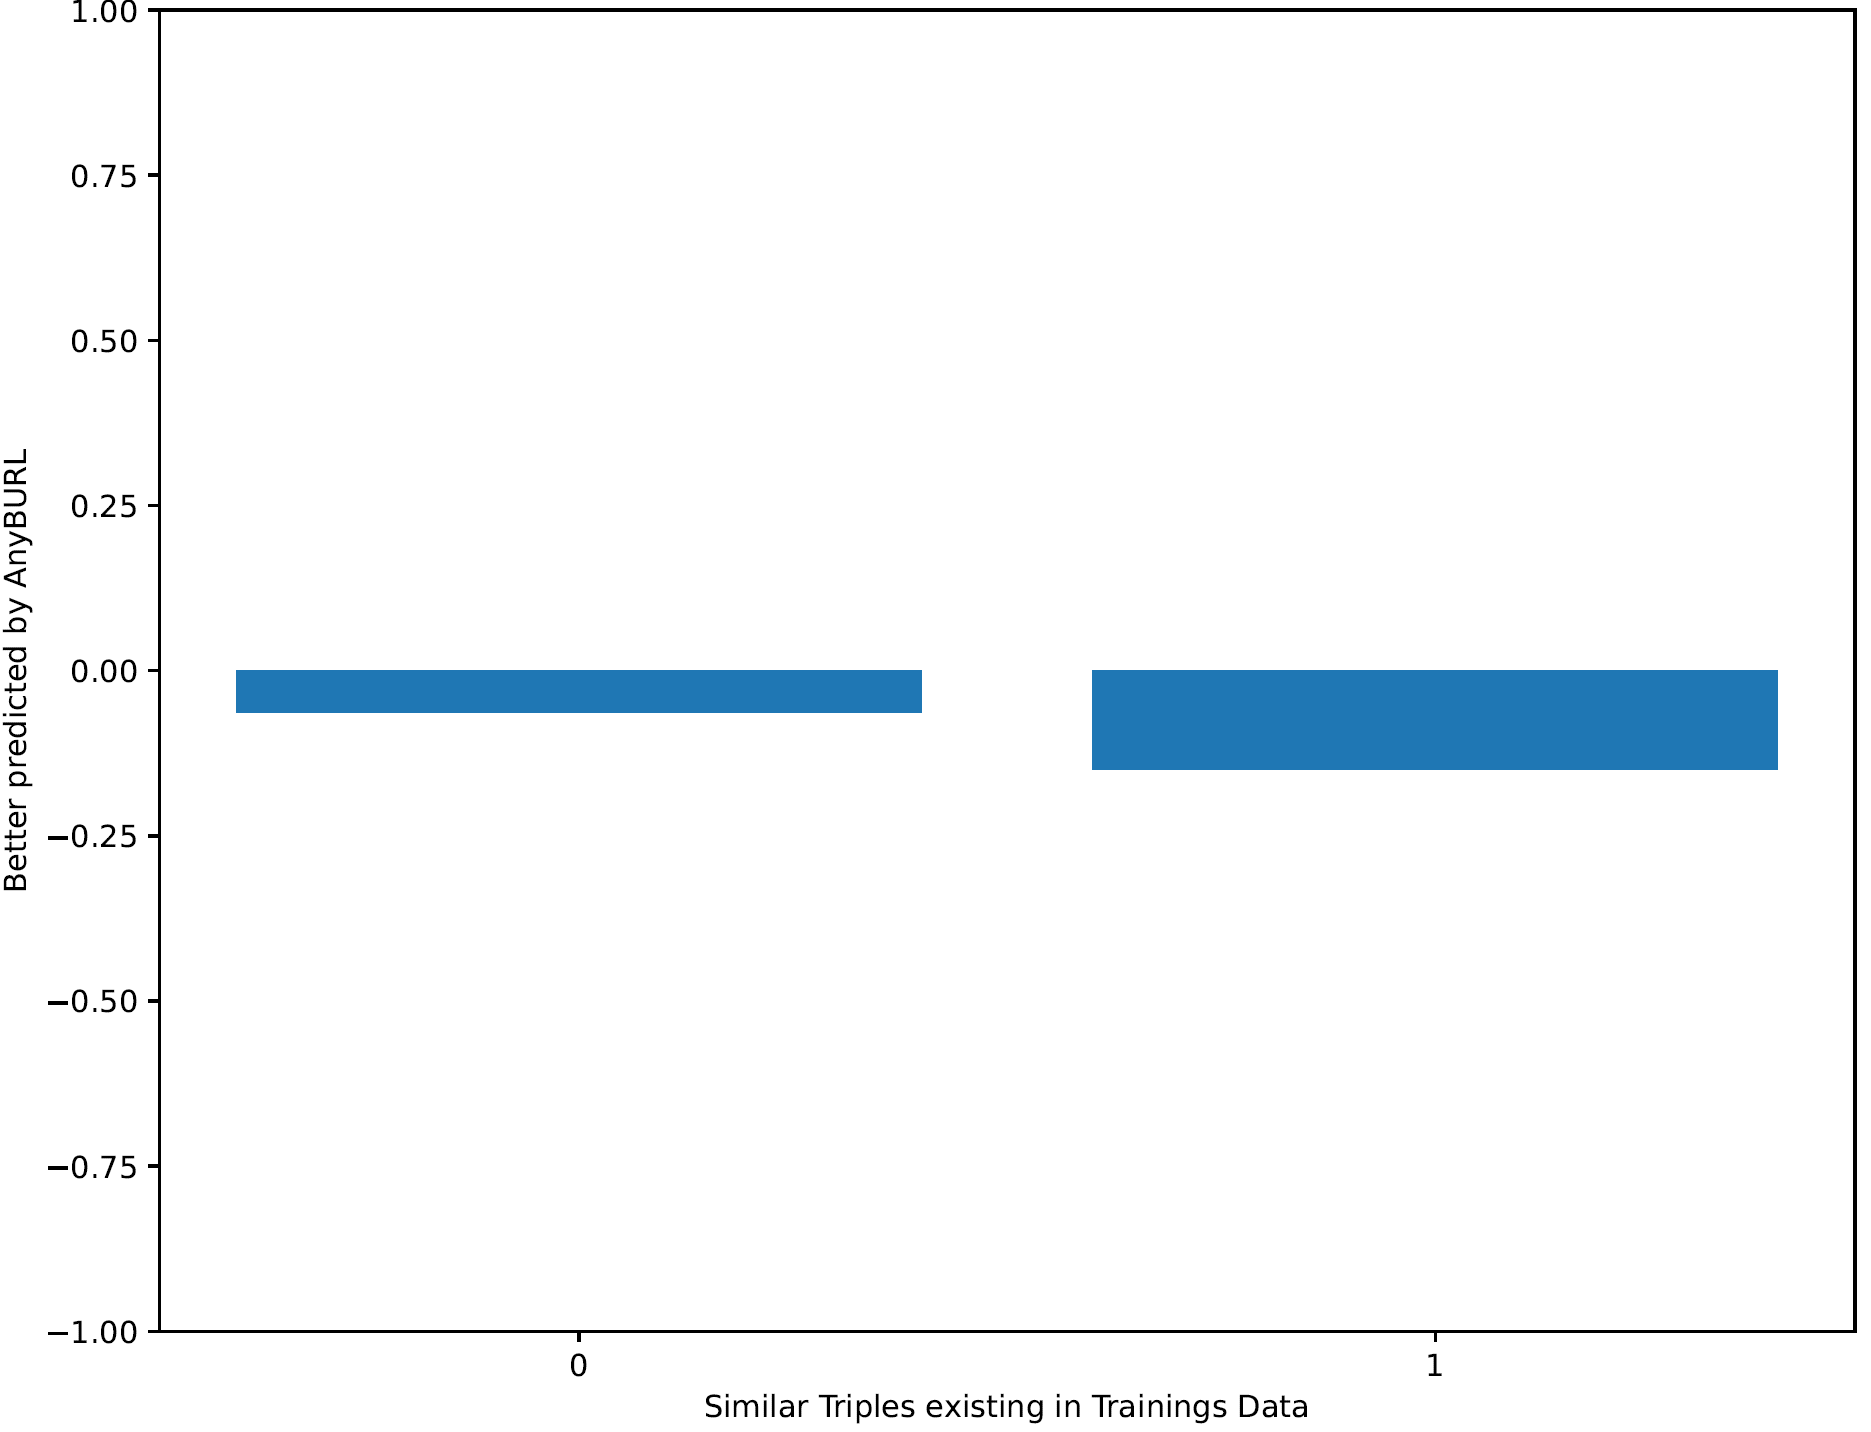
\includegraphics[width=0.9\textwidth]{images/similar_triples_binary_anyburl_complex_fb15k.PNG}
\caption{Comparison of AnyBURL and ComplEx on FB15k-237 in regard to the existence of similar triples in the trainings data}
\label{fig:similar_triples_binary_anyburl_complex_fb15k}
\end{figure}

As argued before having the averaged $better\_predicted\_by$ values this close to $0$ shows that this is not a strong correlation but since all dataset-model combinations produce the same result, I still think that this shows that AnyBURL is slightly better in handling cases where no similar triple exists in the trainings data while the embedding-based models seem to be better in handling cases where such a triple exists.

Based on the previous observations I thought that maybe not only the existence of similar triples could have an influence but that the amount of similar triples might do as well. 

In figure \ref{fig:similar_triples_steps_anyburl_complex_codex} triples are grouped based on the amount of similar triples existing in the trainings data. I would have expected for the $better\_predicted\_by$ value to continuously decrease. While there is a decrease initially for an higher amount of similar triples his pattern does not continue throughout figure with the value starting to increase again after more than $80$ similar triples. 

\begin{figure}[H]
\centering
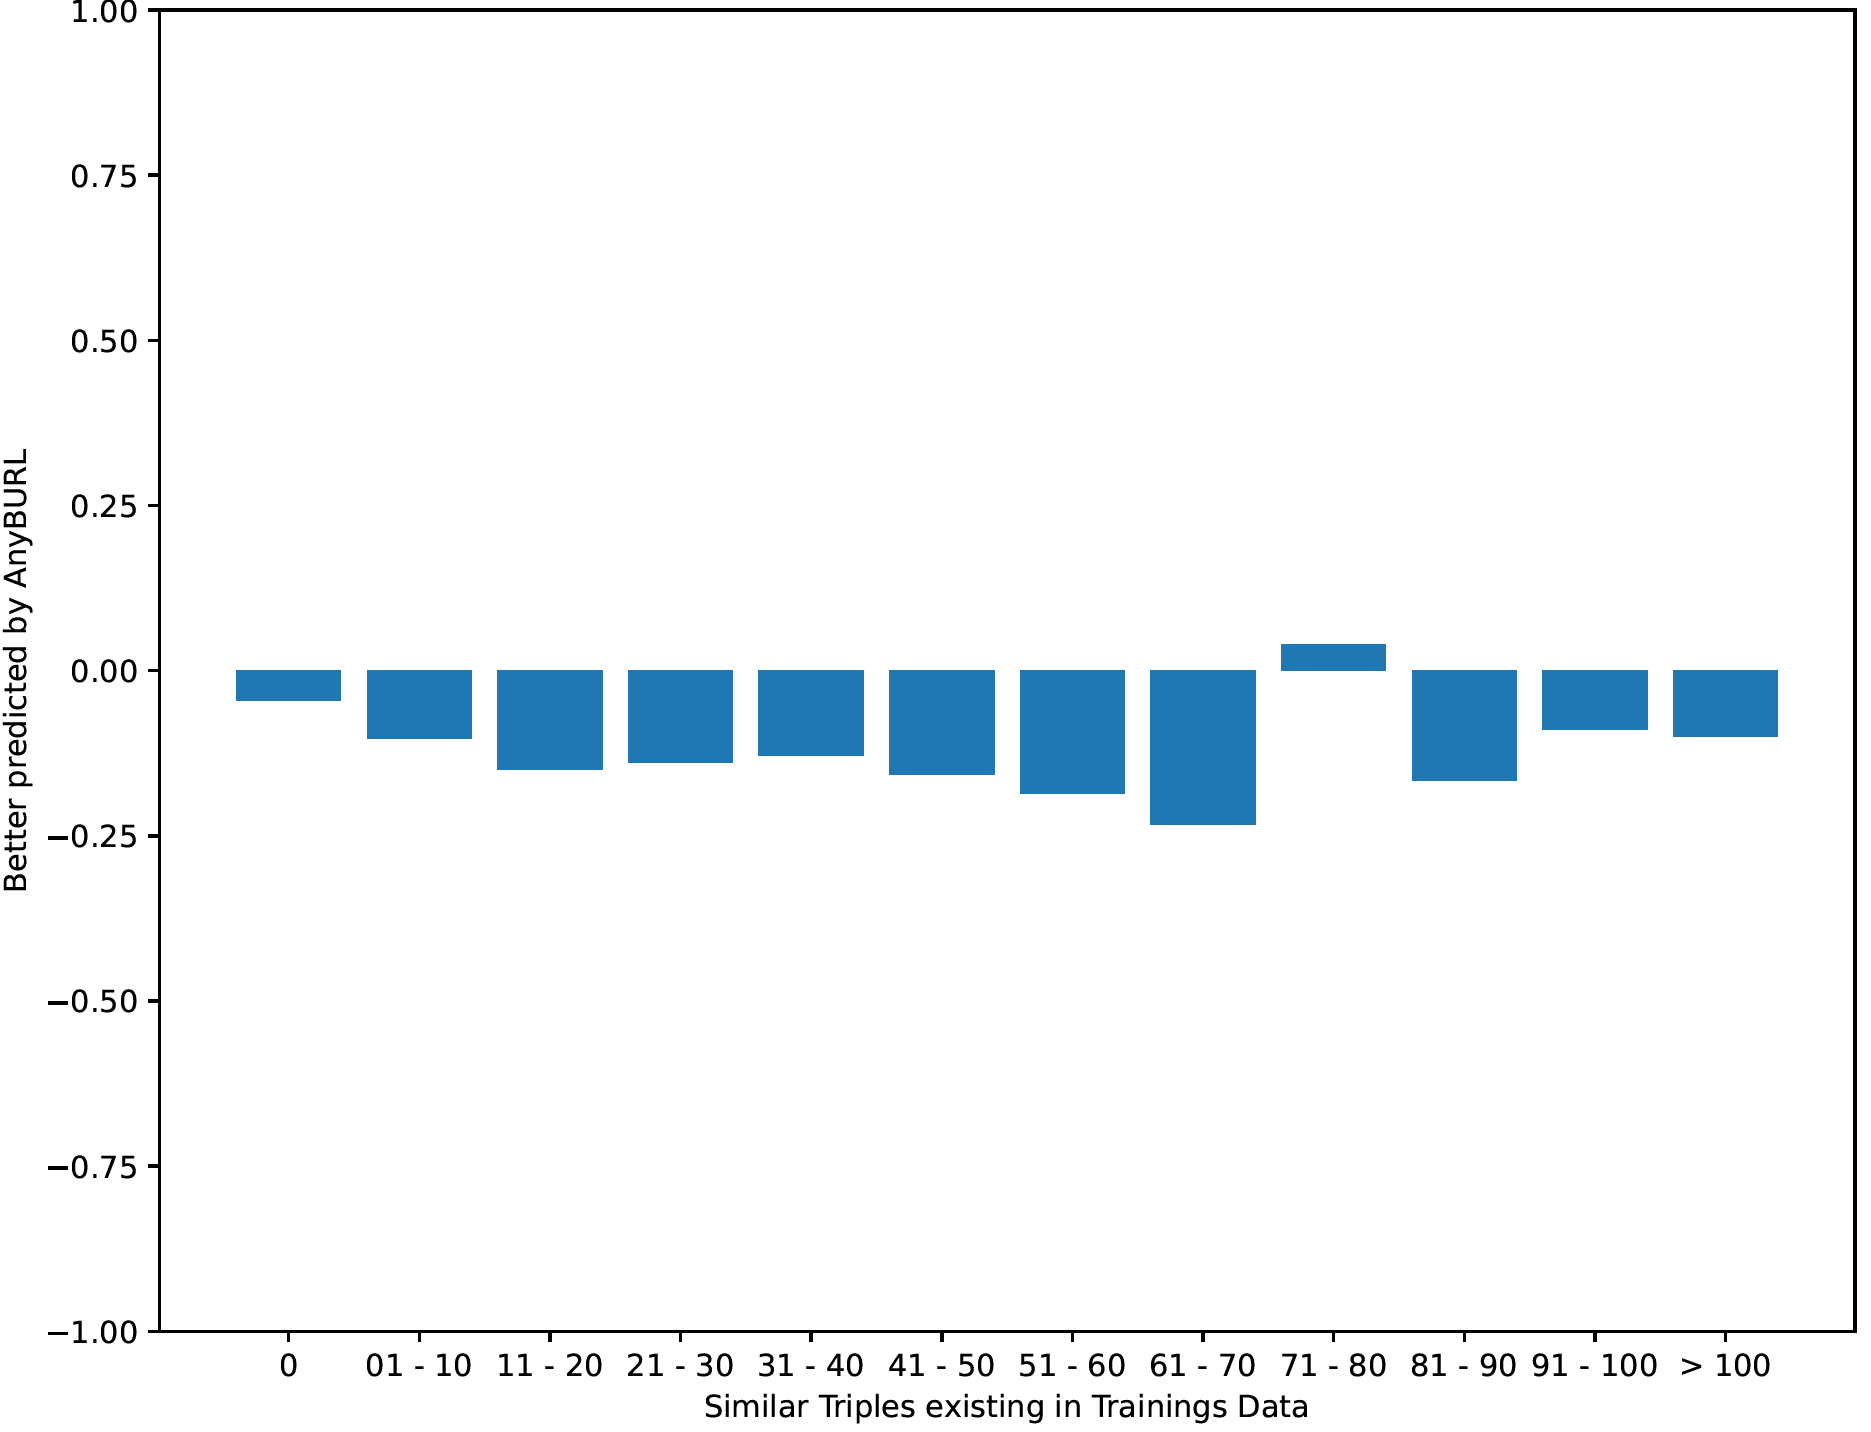
\includegraphics[width=0.9\textwidth]{images/similar_triples_steps_anyburl_complex_codex.PNG}
\caption{Comparison of AnyBURL and ComplEx on CodEx-M in regard to the amount of similar triples in the trainings data}
\label{fig:similar_triples_steps_anyburl_complex_codex}
\end{figure}

If we now also consider the data from the other model-dataset combinations, as can be seen in appendix \ref{appendix:similar_triples}, we notice that the average $better\_predicted\_by$ values seem to be more less random without a clear pattern, indicating that the amount seems to have no more influence than the general existence of similar triples.

This part has now shown us that the general existence of similar triples in the trainings data lightly benefits embeddings-based models compared to AnyBURL but the amount of similar triples does not play a larger role.

\subsection{Existence of Similar Entities in the Dataset}
The last characteristic I wanted to investigate is if the existence of similar entities in the dataset has an influence on which approach works better for a triple i.e. whether one approach is better in predicting a triple if for the triple $(h,r,t)$ an entity exists which is similar to either $h$ or $t$.

\subsubsection{Based on the Similarity Score}

To measure the similarity I tried two approaches. In my first one I calculated a cosine similarity matrix between all entity embeddings of the embedding-based model and summed up each row. That resulted in a similarity score for each entity which is higher for entities which have a lot of similar entities and lower for the ones that do not. 

Figure \ref{fig:head_similarity_anyburl_complex_codex} shows the per head entity averaged $better\_predicted\_by$ value with the entity similarity scores for AnyBURL and ComplEx on CoDEx-M. The entities with high similarity scores and the ones with low similarity scores are evenly distributed throughout the figure. Indicating that no model is better than the other in predicting entities with a lot or a few similar entities in the dataset.

\begin{figure}[H]
\centering
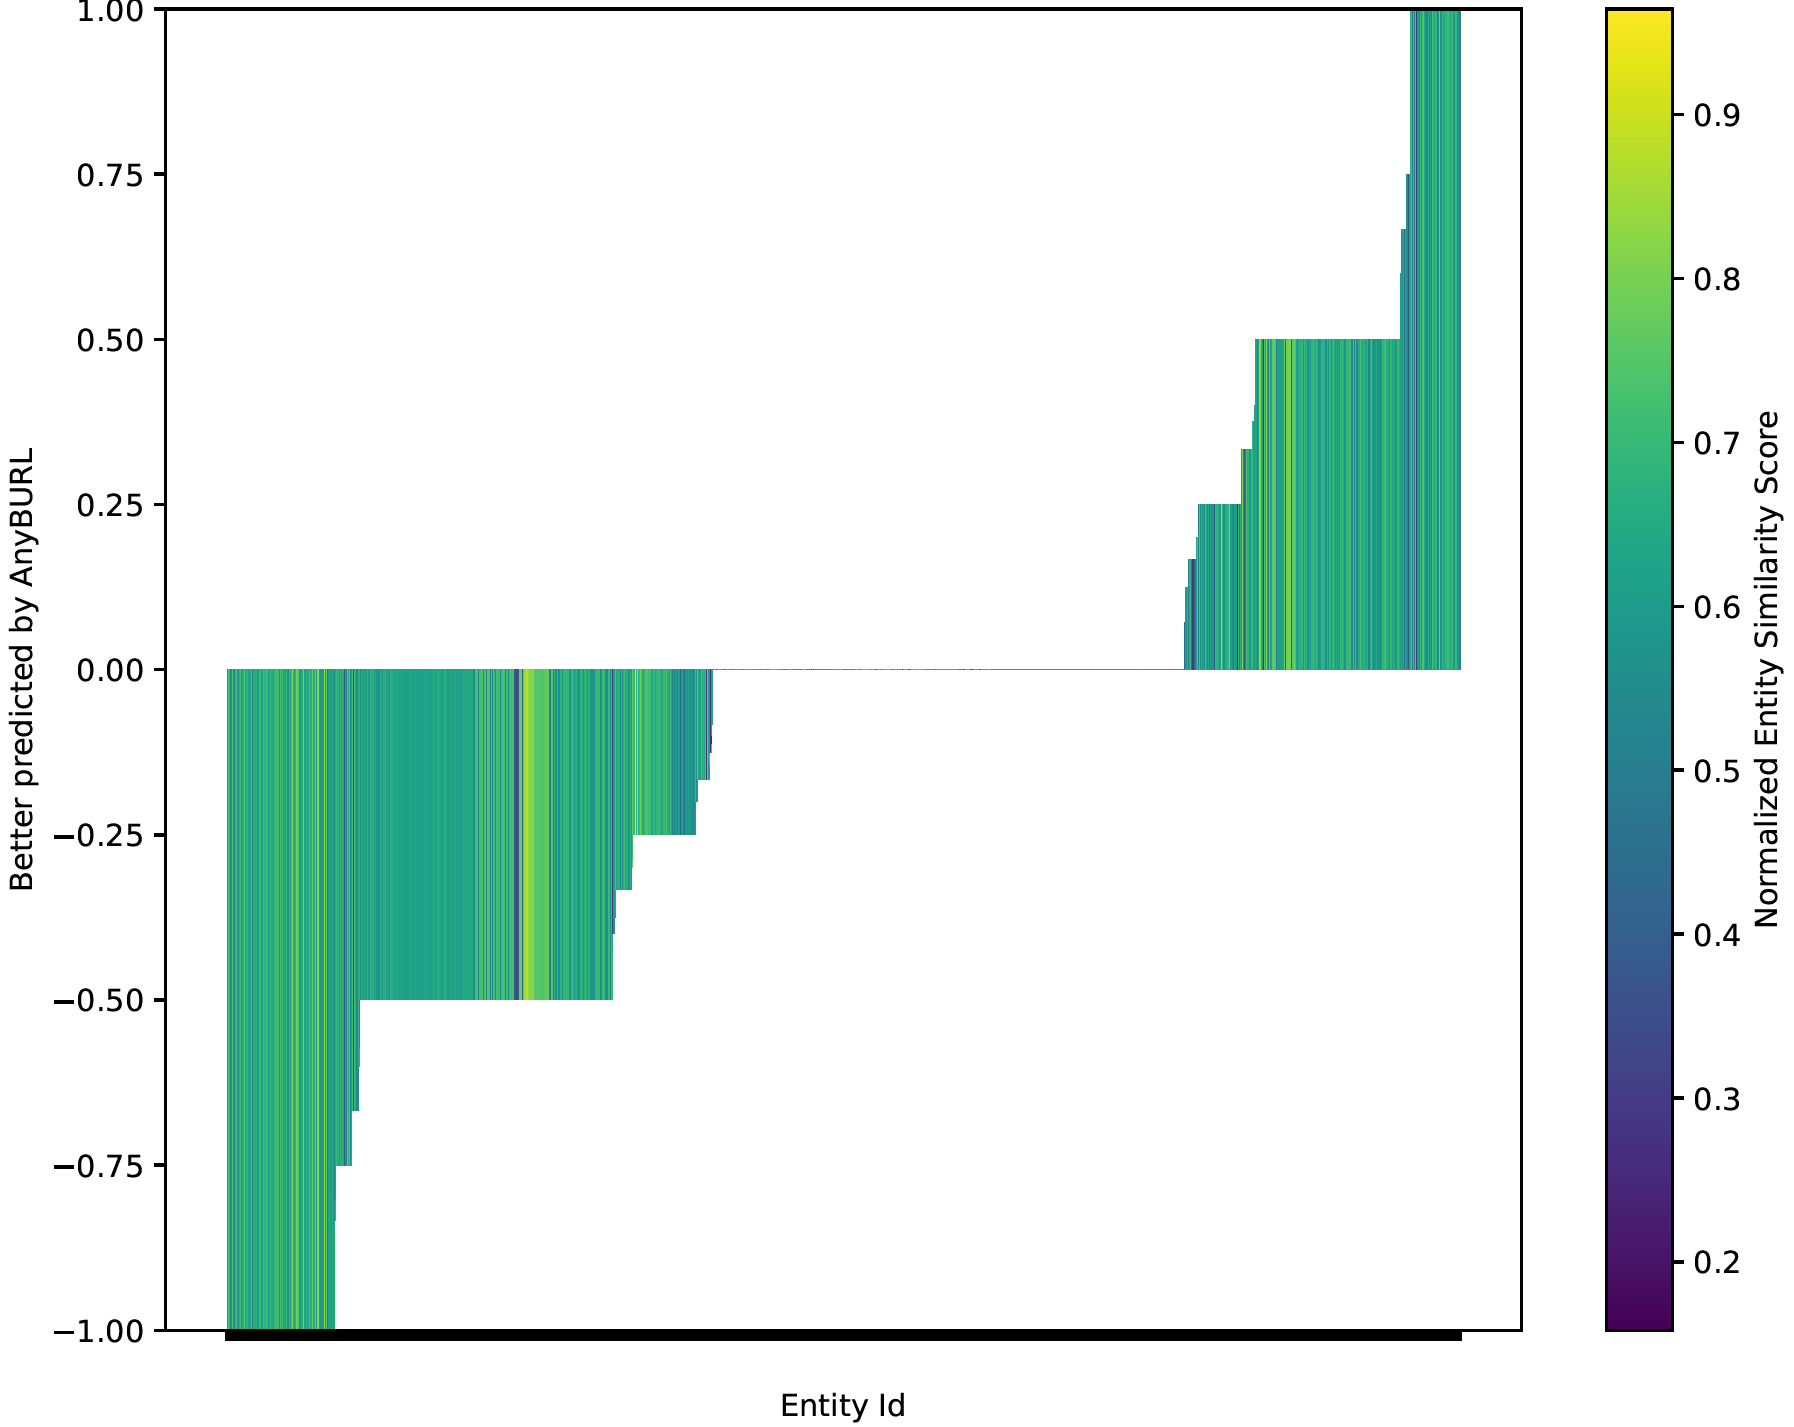
\includegraphics[width=0.7\textwidth]{images/head_similarity_anyburl_complex_codex.PNG}
\caption{Comparison of AnyBURL and ComplEx on CoDEx-M in regard to the existence of similar head entities based on the cosine similarity}
\label{fig:head_similarity_anyburl_complex_codex}
\end{figure}

The same data displayed for the per tail entity averaged $better\_predicted\_by$ values, as can be seen in figure \ref{fig:tail_similarity_anyburl_complex_codex}, has the high and low similarity scores stronger grouped together. The entities with low similarity scores appear mostly in the middle of the figure, indicating that both models predict them equally well, and the ones with a high similarity score have an higher/ lower averaged $better\_predicted\_by$ value showing that they are better predicted by one of the models. Since entities with high similarity appear on both sides we can not conclude that either model is better in predicting triples containing entities for which a lot of similar entities are included in the dataset. 

\begin{figure}[H]
\centering
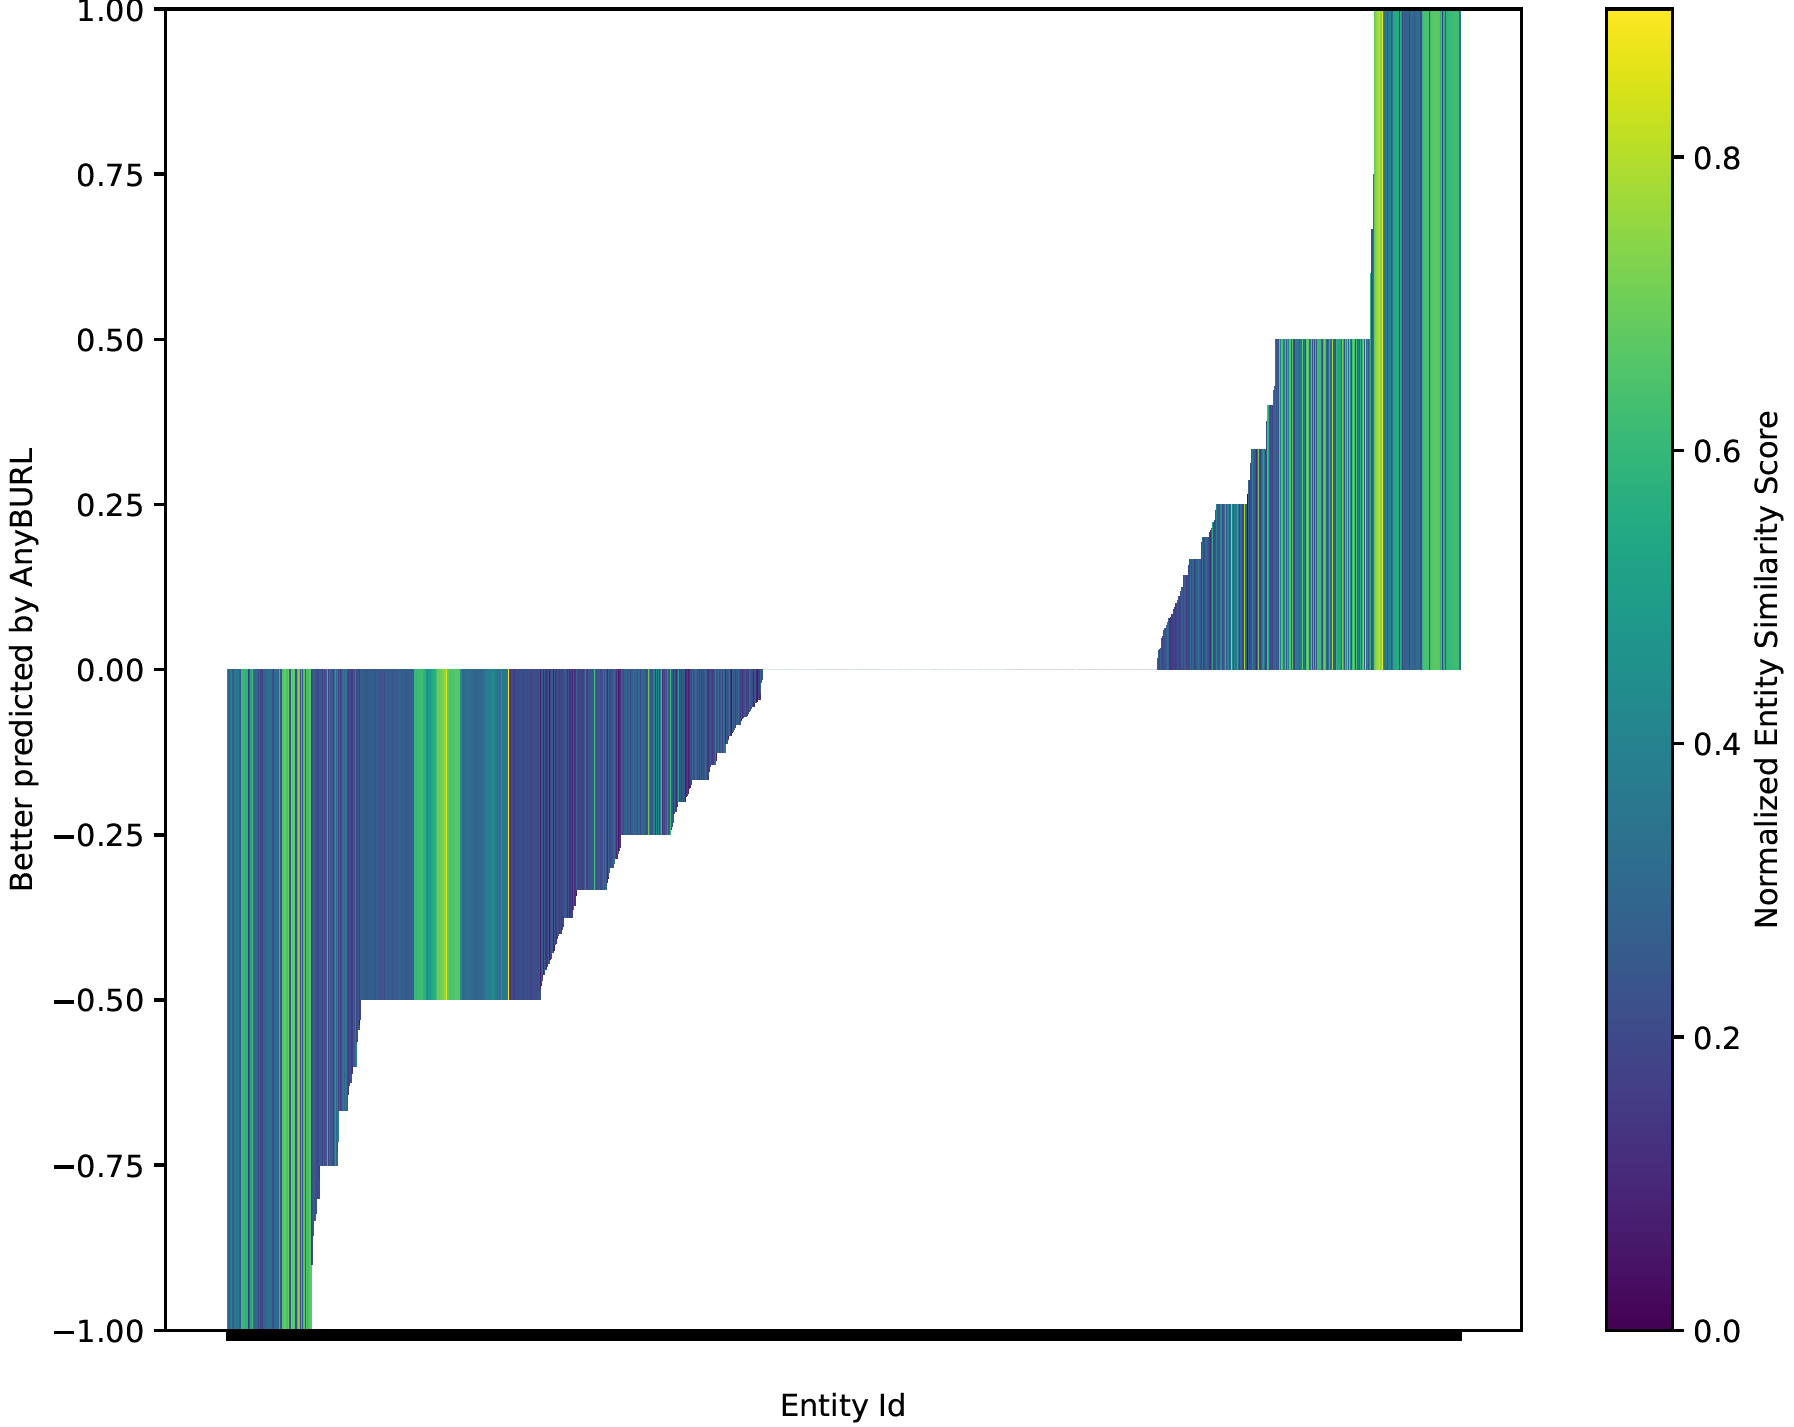
\includegraphics[width=0.7\textwidth]{images/tail_similarity_anyburl_complex_codex.PNG}
\caption{Comparison of AnyBURL and ComplEx on CoDEx-M in regard to the existence of similar tail entities based on the cosine similarity}
\label{fig:tail_similarity_anyburl_complex_codex}
\end{figure}

But it is still interesting that entities with high similarity scores are better predicted by one of the models. Maybe the models are learning specific groups better than the other model. To further investigate this I tried to cluster the entities in the next section.

\subsubsection{Based on K-Means Clustering}
To cluster the entities I applied K-means clustering onto the entity embeddings. I tried different cluster sizes and in the end a cluster size of $k=100$ proved to create the comprehensible results. 

Important to note here is that while I tried all embedding-based models to create clusters, the clusters in the upcoming figures are always the ones based on the ComplEx embeddings e.g. in figure \ref{fig:tail_cluster_100_anyburl_conve_codex} AnyBURL and ConvE are compared but the clusters are based on ComplEx. I made this decision to be better able to compare the clusters across different embedding-based models. Furthermore, we have the option of assigning a triple to a cluster either based on its head or tail entity. In the previous section we have seen that the similarity score works best if it is assigned based on the tail entity and the same goes for the clustering here. In appendix \ref{appendix:similar_entities} we can also see the clustering based on the heads but the results based on the tails are more useful and therefore in the following I will only address these.

In figure \ref{fig:tail_cluster_100_anyburl_complex_codex} we can see the averaged $better\_predicted\_by$ value per cluster for AnyBURL and ComplEx on CoDEx-M. There are clusters which are clearly better predicted by one of the models. While the largest clusters are tending towards a $better\_predicted\_by$ value of $0$ the clusters tending towards either of the models still contain a few triples. It is an interesting result that some entities, which are in the eyes of the ComplEx embeddings similar, are clearly better predicted by one of the models.

\begin{figure}[H]
\centering
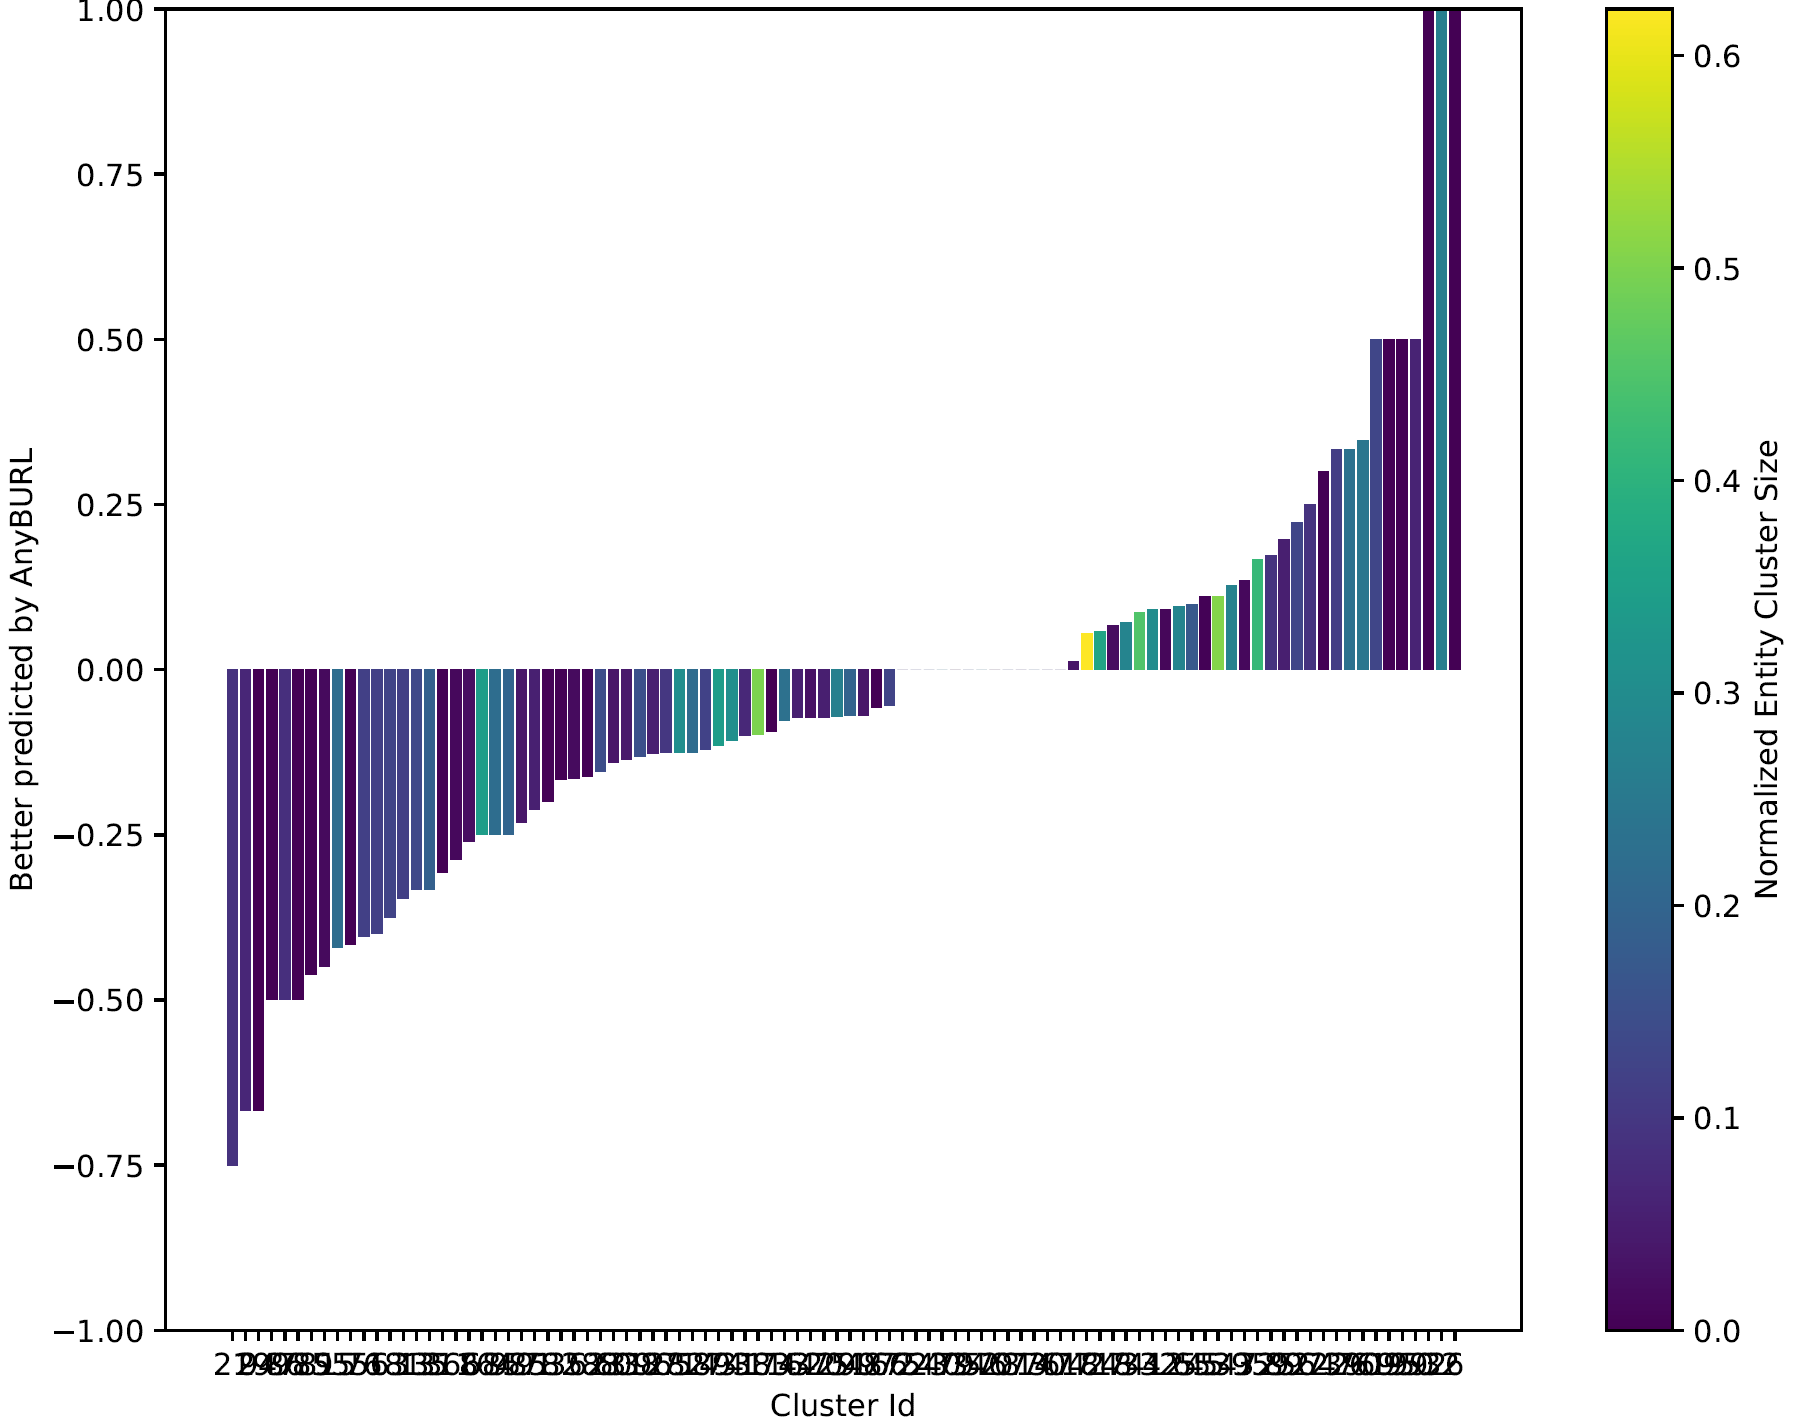
\includegraphics[width=0.9\textwidth]{images/tail_cluster_100_anyburl_complex_codex.PNG}
\caption{Comparison of AnyBURL and ComplEx on CoDEx-M in regard to the existence of similar tail entities based on K-Means Clustering (k=100)}
\label{fig:tail_cluster_100_anyburl_complex_codex}
\end{figure}

In figure \ref{fig:tail_cluster_100_anyburl_conve_rescal_codex} we can see the same comparison for AnyBURL and ConvE/ RESCAL on CoDEx-M. Here there are also clearly a few clusters better predicted by one of the models. What can not be seen in these figures is that the clusters tending towards either AnyBURL or one of the embedding-based models are the same clusters across all three comparisons. Showing that these clusters are a group of tails which are easier to predict for one of the approaches.  

\begin{figure}[H]
\centering
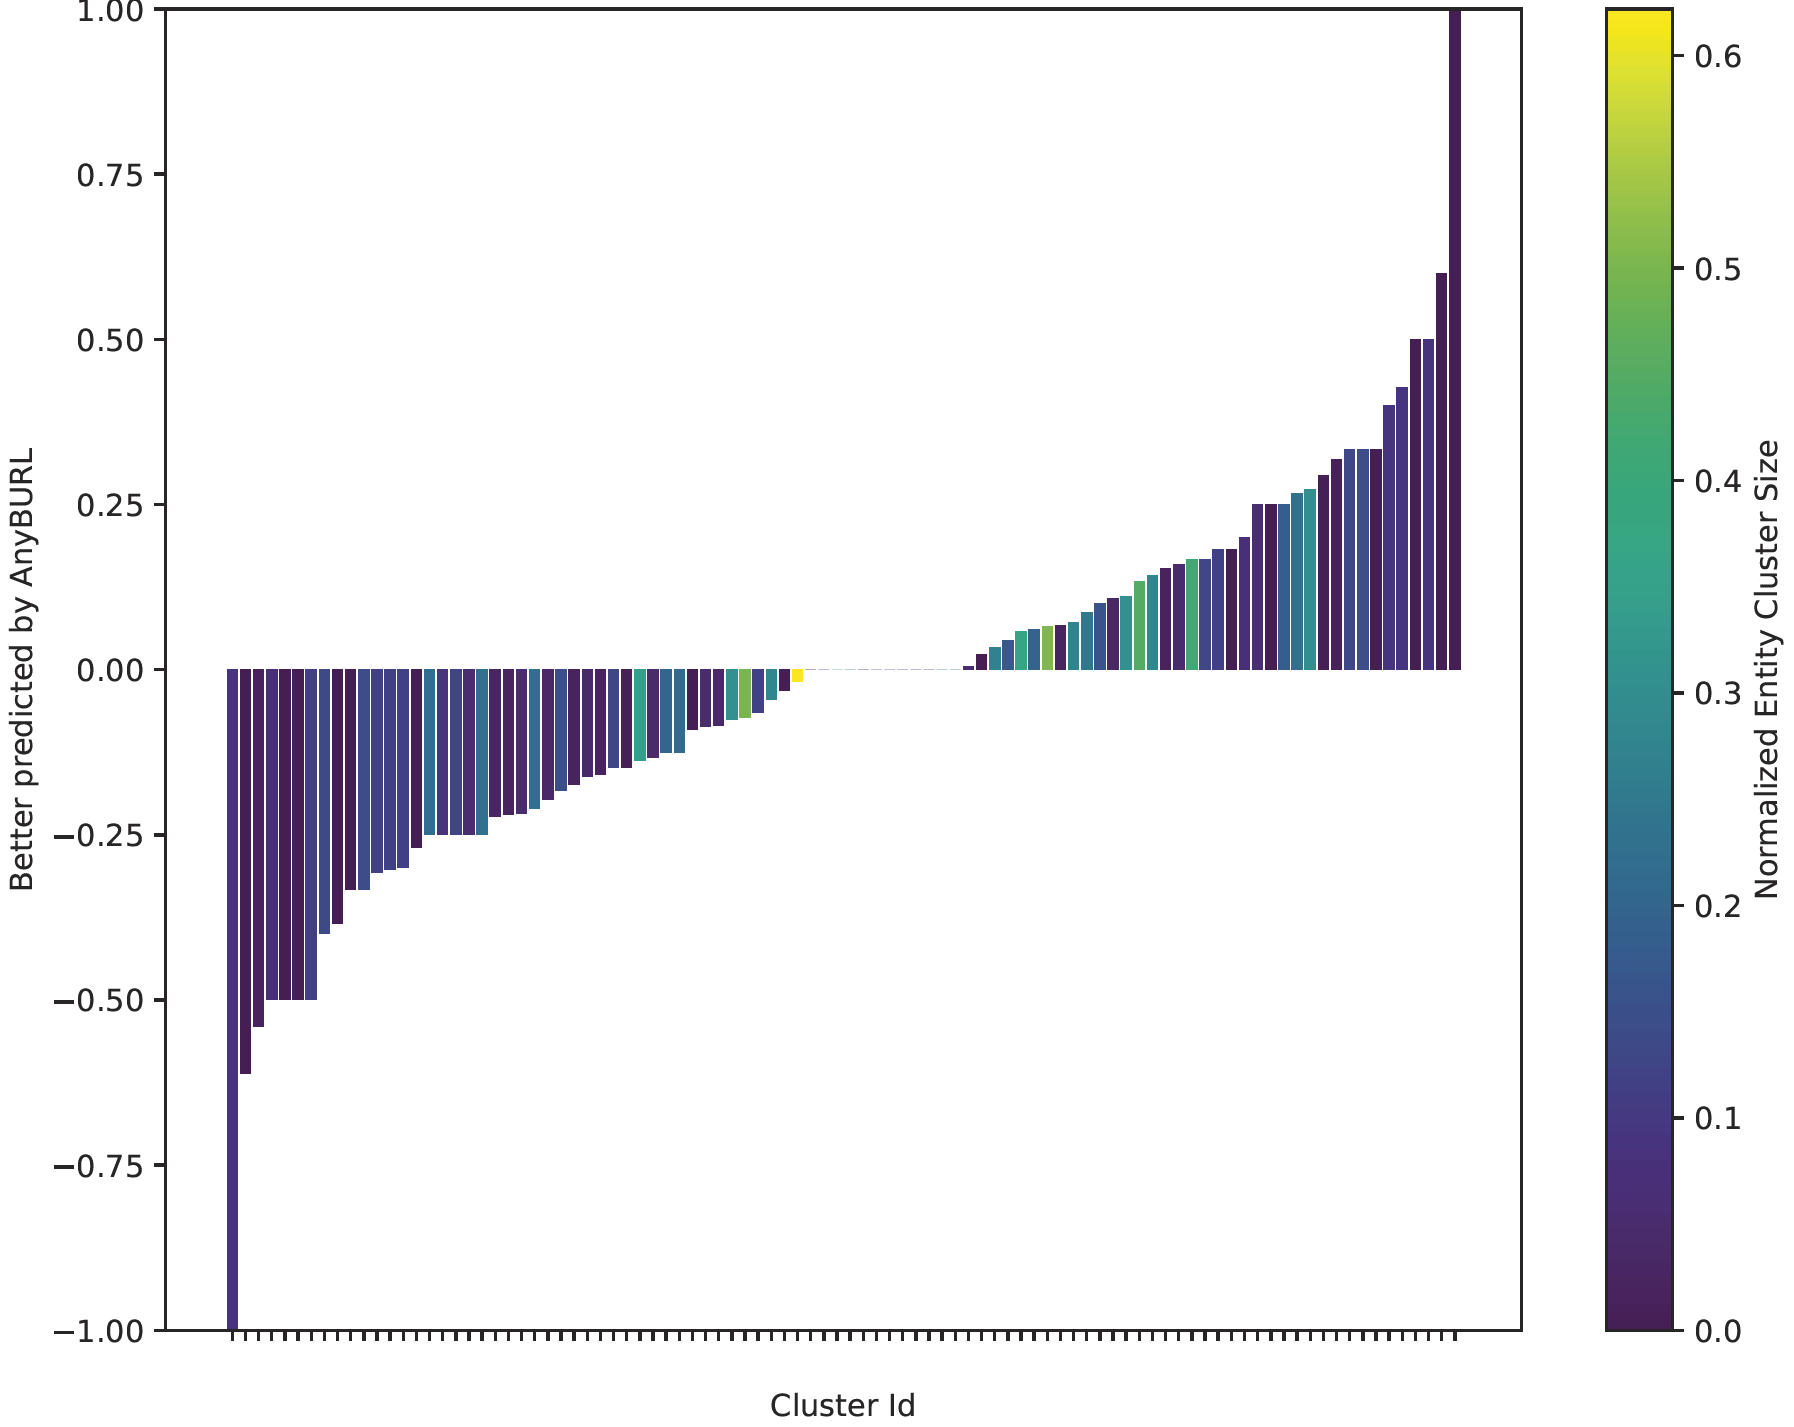
\includegraphics[width=0.45\textwidth]{images/tail_cluster_100_anyburl_conve_codex.PNG}
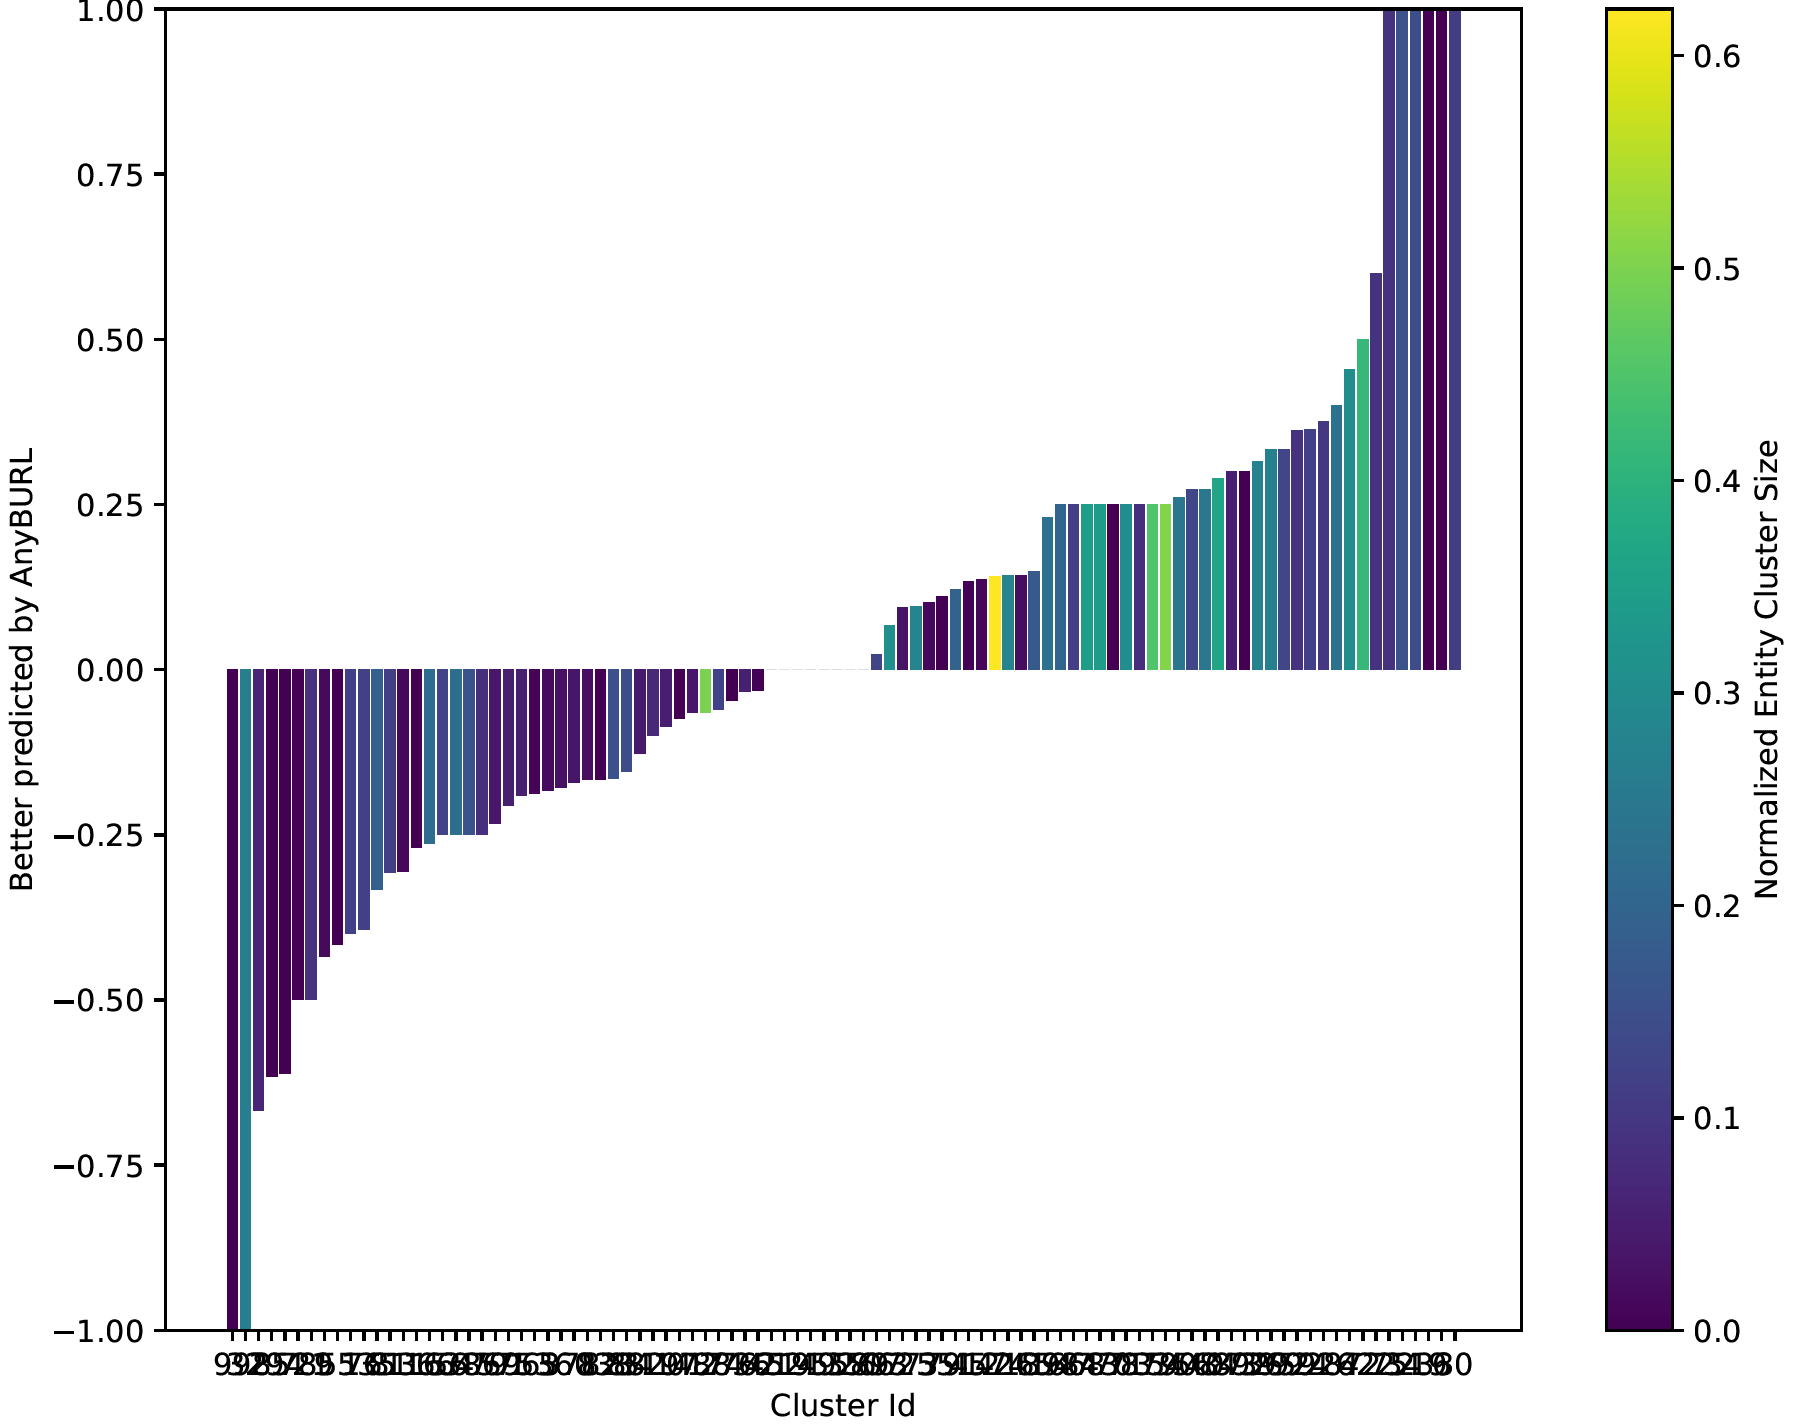
\includegraphics[width=0.45\textwidth]{images/tail_cluster_100_anyburl_rescal_codex.PNG}
\caption{Comparison of AnyBURL and ConvE (left)/ RESCAL (right) on CoDEx-M in regard to the existence of similar tail entities based on K-Means Clustering (k=100)}
\label{fig:tail_cluster_100_anyburl_conve_rescal_codex}
\end{figure}

Doing the same analysis on FB15k-237 shows less expressive results than on CoDEx-M. While here some clusters tend more towards on of the models all averaged $better\_predicted\_by$ values are quiet low. This indicates that neither of the models predict a cluster significantly better than the other. This can be seen in figure \ref{fig:tail_cluster_100_anyburl_complex_fb15k} for AnyBURL and ComplEx and for the other models the same figure can be found in appendix \ref{appendix:similar_entities}.

\begin{figure}[H]
\centering
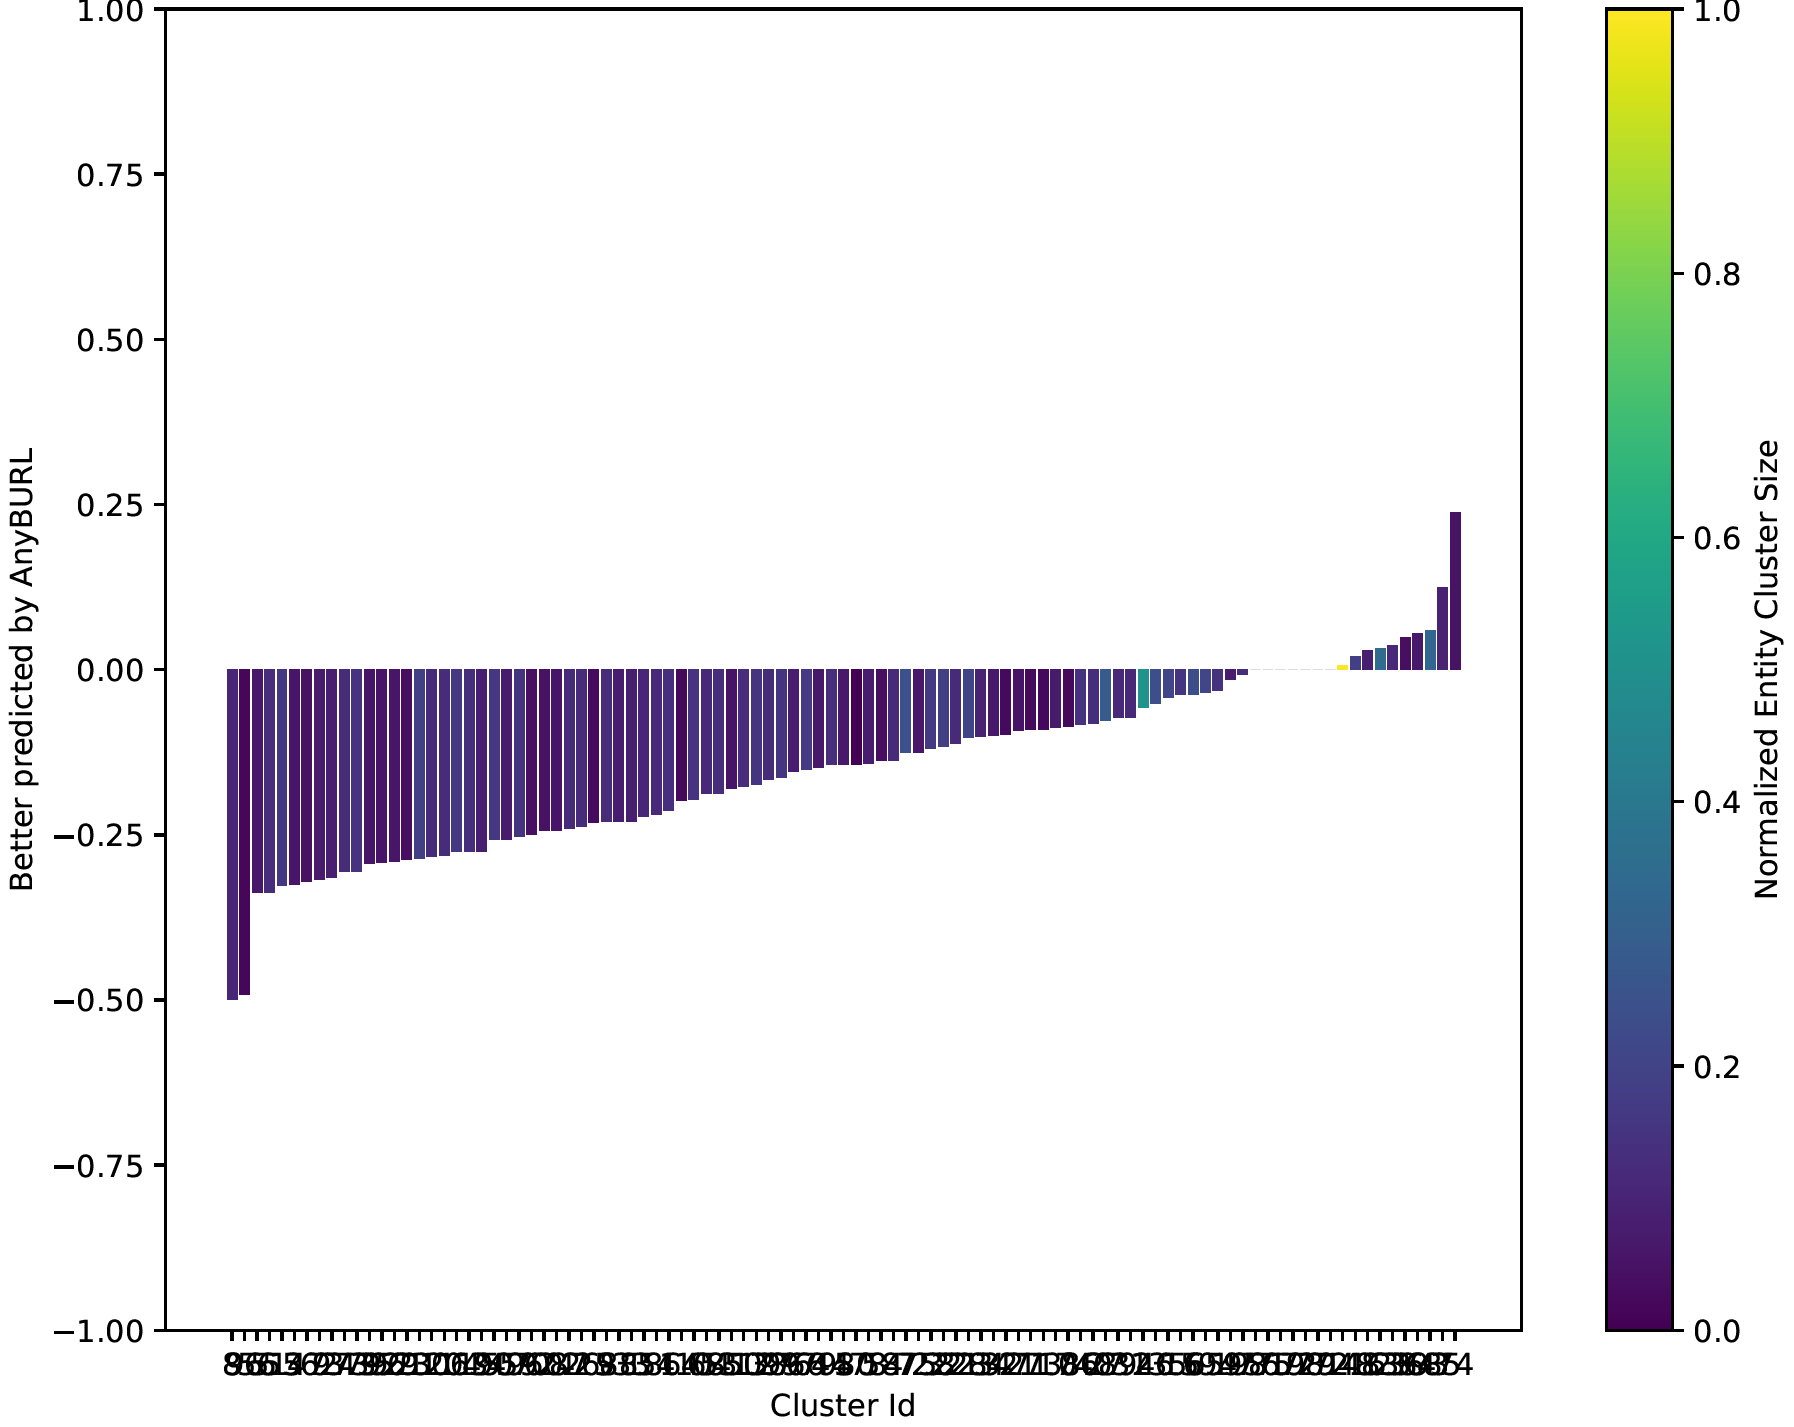
\includegraphics[width=0.8\textwidth]{images/tail_cluster_100_anyburl_complex_fb15k.PNG}
\caption{Comparison of AnyBURL and ComplEx on FB15k-237 in regard to the existence of similar tail entities based on K-Means Clustering (k=100)}
\label{fig:tail_cluster_100_anyburl_complex_fb15k}
\end{figure}

On YAGO3-10 on the other hand clusters were found which can be clearly assigned to one of the approaches. In figure \ref{fig:tail_cluster_100_anyburl_complex_yago} we can see that different from the result from CoDEx-M that for YAGO3-10 there larger clusters clearly better predicted by one of the approaches. For example the largest cluster has an average $better\_predicted\_by$ of above $0.95$ and is therefore clearly better predicted by AnyBURL.

\begin{figure}[H]
\centering
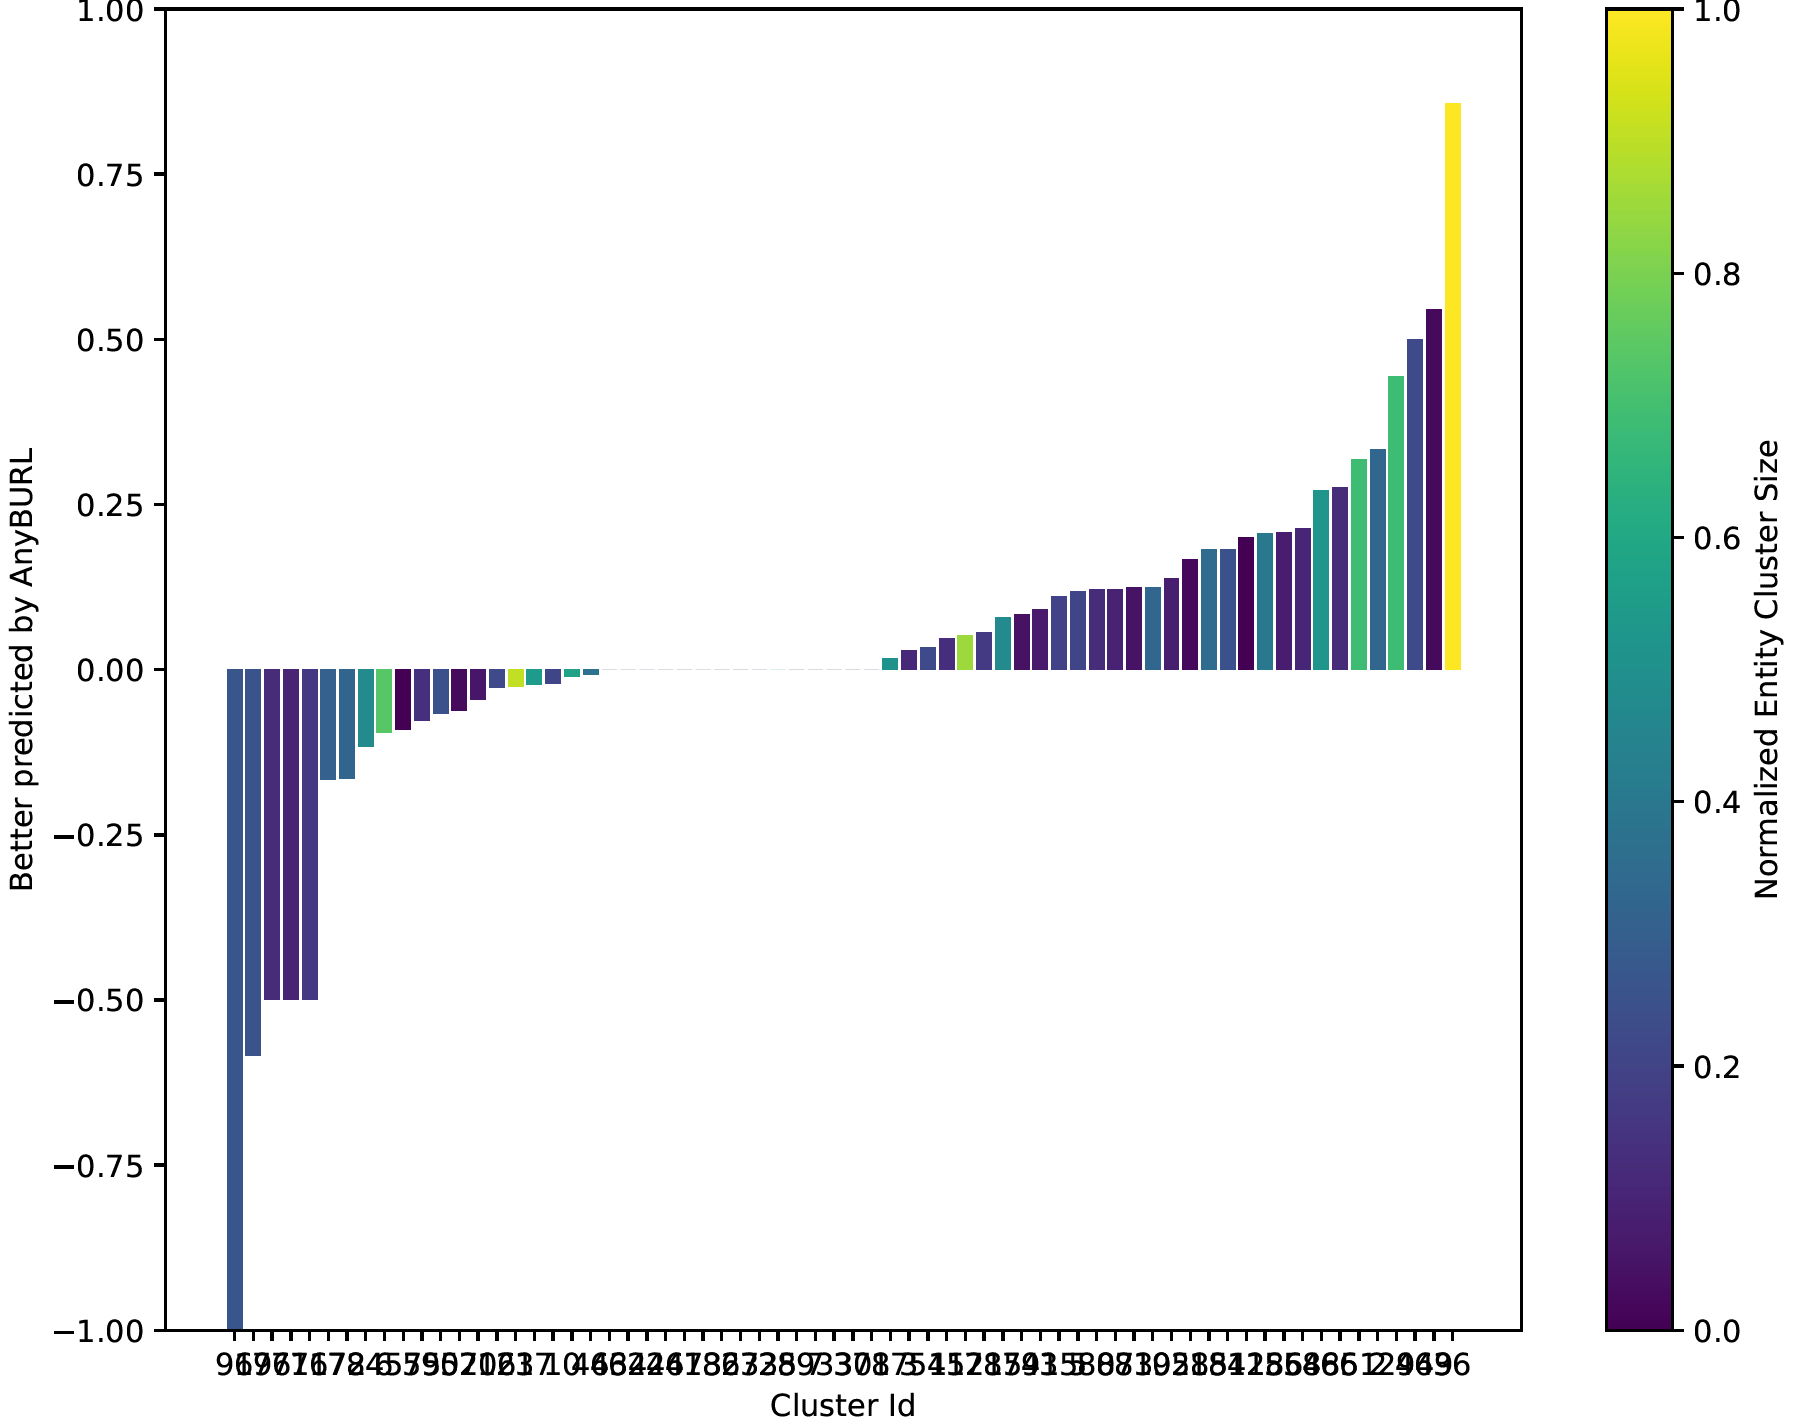
\includegraphics[width=0.9\textwidth]{images/tail_cluster_100_anyburl_complex_yago.PNG}
\caption{Comparison of AnyBURL and ComplEx on YAGO3-10 in regard to the existence of similar tail entities based on K-Means Clustering (k=100)}
\label{fig:tail_cluster_100_anyburl_complex_yago}
\end{figure}



